\documentclass[twoside]{book}

% Packages required by doxygen
\usepackage{fixltx2e}
\usepackage{calc}
\usepackage{doxygen}
\usepackage[export]{adjustbox} % also loads graphicx
\usepackage{graphicx}
\usepackage[utf8]{inputenc}
\usepackage{makeidx}
\usepackage{multicol}
\usepackage{multirow}
\PassOptionsToPackage{warn}{textcomp}
\usepackage{textcomp}
\usepackage[nointegrals]{wasysym}
\usepackage[table]{xcolor}

% Font selection
\usepackage[T1]{fontenc}
\usepackage[scaled=.90]{helvet}
\usepackage{courier}
\usepackage{amssymb}
\usepackage{sectsty}
\renewcommand{\familydefault}{\sfdefault}
\allsectionsfont{%
  \fontseries{bc}\selectfont%
  \color{darkgray}%
}
\renewcommand{\DoxyLabelFont}{%
  \fontseries{bc}\selectfont%
  \color{darkgray}%
}
\newcommand{\+}{\discretionary{\mbox{\scriptsize$\hookleftarrow$}}{}{}}

% Page & text layout
\usepackage{geometry}
\geometry{%
  a4paper,%
  top=2.5cm,%
  bottom=2.5cm,%
  left=2.5cm,%
  right=2.5cm%
}
\tolerance=750
\hfuzz=15pt
\hbadness=750
\setlength{\emergencystretch}{15pt}
\setlength{\parindent}{0cm}
\setlength{\parskip}{3ex plus 2ex minus 2ex}
\makeatletter
\renewcommand{\paragraph}{%
  \@startsection{paragraph}{4}{0ex}{-1.0ex}{1.0ex}{%
    \normalfont\normalsize\bfseries\SS@parafont%
  }%
}
\renewcommand{\subparagraph}{%
  \@startsection{subparagraph}{5}{0ex}{-1.0ex}{1.0ex}{%
    \normalfont\normalsize\bfseries\SS@subparafont%
  }%
}
\makeatother

% Headers & footers
\usepackage{fancyhdr}
\pagestyle{fancyplain}
\fancyhead[LE]{\fancyplain{}{\bfseries\thepage}}
\fancyhead[CE]{\fancyplain{}{}}
\fancyhead[RE]{\fancyplain{}{\bfseries\leftmark}}
\fancyhead[LO]{\fancyplain{}{\bfseries\rightmark}}
\fancyhead[CO]{\fancyplain{}{}}
\fancyhead[RO]{\fancyplain{}{\bfseries\thepage}}
\fancyfoot[LE]{\fancyplain{}{}}
\fancyfoot[CE]{\fancyplain{}{}}
\fancyfoot[RE]{\fancyplain{}{\bfseries\scriptsize Generated by Doxygen }}
\fancyfoot[LO]{\fancyplain{}{\bfseries\scriptsize Generated by Doxygen }}
\fancyfoot[CO]{\fancyplain{}{}}
\fancyfoot[RO]{\fancyplain{}{}}
\renewcommand{\footrulewidth}{0.4pt}
\renewcommand{\chaptermark}[1]{%
  \markboth{#1}{}%
}
\renewcommand{\sectionmark}[1]{%
  \markright{\thesection\ #1}%
}

% Indices & bibliography
\usepackage{natbib}
\usepackage[titles]{tocloft}
\setcounter{tocdepth}{3}
\setcounter{secnumdepth}{5}
\makeindex

% Hyperlinks (required, but should be loaded last)
\usepackage{ifpdf}
\ifpdf
  \usepackage[pdftex,pagebackref=true]{hyperref}
\else
  \usepackage[ps2pdf,pagebackref=true]{hyperref}
\fi
\hypersetup{%
  colorlinks=true,%
  linkcolor=blue,%
  citecolor=blue,%
  unicode%
}

% Custom commands
\newcommand{\clearemptydoublepage}{%
  \newpage{\pagestyle{empty}\cleardoublepage}%
}

\usepackage{caption}
\captionsetup{labelsep=space,justification=centering,font={bf},singlelinecheck=off,skip=4pt,position=top}

%===== C O N T E N T S =====

\begin{document}

% Titlepage & ToC
\hypersetup{pageanchor=false,
             bookmarksnumbered=true,
             pdfencoding=unicode
            }
\pagenumbering{roman}
\begin{titlepage}
\vspace*{7cm}
\begin{center}%
{\Large Greedy\+Herwig7 }\\
\vspace*{1cm}
{\large Generated by Doxygen 1.8.11}\\
\end{center}
\end{titlepage}
\clearemptydoublepage
\tableofcontents
\clearemptydoublepage
\pagenumbering{arabic}
\hypersetup{pageanchor=true}

%--- Begin generated contents ---
\chapter{A handle for saving Herwig 7 events into R\+O\+OT trees}
\label{index}\hypertarget{index}{}\input{index}
\chapter{Namespace Index}
\section{Namespace List}
Here is a list of all namespaces with brief descriptions\+:\begin{DoxyCompactList}
\item\contentsline{section}{\hyperlink{namespacecfg}{cfg} \\*Configuration settings }{\pageref{namespacecfg}}{}
\item\contentsline{section}{\hyperlink{namespace_hadr_funcs}{Hadr\+Funcs} \\*Some functions for P\+DG particle code recognition for hadrons }{\pageref{namespace_hadr_funcs}}{}
\item\contentsline{section}{\hyperlink{namespace_herwig}{Herwig} \\*The standard Herwig7 namespace }{\pageref{namespace_herwig}}{}
\item\contentsline{section}{\hyperlink{namespacesettings}{settings} \\*A python-\/based script for generating a Herwig7 settings file }{\pageref{namespacesettings}}{}
\item\contentsline{section}{\hyperlink{namespace_the_p_e_g}{The\+P\+EG} \\*\hyperlink{namespace_the_p_e_g}{The\+P\+EG} is the basic infrastructure, on which Herwig7 is built }{\pageref{namespace_the_p_e_g}}{}
\end{DoxyCompactList}

\chapter{Hierarchical Index}
\section{Class Hierarchy}
This inheritance list is sorted roughly, but not completely, alphabetically\+:\begin{DoxyCompactList}
\item Analysis\+Handler\begin{DoxyCompactList}
\item \contentsline{section}{Herwig\+:\+:Herwig\+Tree}{\pageref{class_herwig_1_1_herwig_tree}}{}
\end{DoxyCompactList}
\item \contentsline{section}{Parton\+Holder}{\pageref{struct_parton_holder}}{}
\item \contentsline{section}{Timer}{\pageref{class_timer}}{}
\item T\+Object\begin{DoxyCompactList}
\item \contentsline{section}{Prtcl\+Data}{\pageref{class_prtcl_data}}{}
\item \contentsline{section}{Prtcl\+Event}{\pageref{class_prtcl_event}}{}
\end{DoxyCompactList}
\item \contentsline{section}{Herwig\+:\+:T\+T\+Bar}{\pageref{struct_herwig_1_1_t_t_bar}}{}
\end{DoxyCompactList}

\chapter{Class Index}
\section{Class List}
Here are the classes, structs, unions and interfaces with brief descriptions\+:\begin{DoxyCompactList}
\item\contentsline{section}{\hyperlink{class_herwig_1_1_herwig_tree}{Herwig\+::\+Herwig\+Tree} \\*The main class handle for the Herwig7 analysis }{\pageref{class_herwig_1_1_herwig_tree}}{}
\item\contentsline{section}{\hyperlink{struct_parton_holder}{Parton\+Holder} \\*A struct for storing parton information }{\pageref{struct_parton_holder}}{}
\item\contentsline{section}{\hyperlink{class_prtcl_data}{Prtcl\+Data} }{\pageref{class_prtcl_data}}{}
\item\contentsline{section}{\hyperlink{class_prtcl_event}{Prtcl\+Event} }{\pageref{class_prtcl_event}}{}
\item\contentsline{section}{\hyperlink{class_timer}{Timer} \\*Timing class for showing the progress of a simulation }{\pageref{class_timer}}{}
\item\contentsline{section}{\hyperlink{struct_herwig_1_1_t_t_bar}{Herwig\+::\+T\+T\+Bar} \\*A custom selector to be used with Herwig7. Not used, here for future reference }{\pageref{struct_herwig_1_1_t_t_bar}}{}
\end{DoxyCompactList}

\chapter{File Index}
\section{File List}
Here is a list of all files with brief descriptions\+:\begin{DoxyCompactList}
\item\contentsline{section}{/work/hsiikone/development/gen\+\_\+handle/\hyperlink{greedy__settings_8h}{greedy\+\_\+settings.\+h} }{\pageref{greedy__settings_8h}}{}
\item\contentsline{section}{/work/hsiikone/development/gen\+\_\+handle/events/\hyperlink{_prtcl_event_8h}{Prtcl\+Event.\+h} }{\pageref{_prtcl_event_8h}}{}
\item\contentsline{section}{/work/hsiikone/development/gen\+\_\+handle/generic/\hyperlink{help__functions_8h}{help\+\_\+functions.\+h} }{\pageref{help__functions_8h}}{}
\item\contentsline{section}{/work/hsiikone/development/gen\+\_\+handle/greedy\+\_\+herwig7/\hyperlink{_herwig_tree_8cpp}{Herwig\+Tree.\+cpp} }{\pageref{_herwig_tree_8cpp}}{}
\item\contentsline{section}{/work/hsiikone/development/gen\+\_\+handle/greedy\+\_\+herwig7/\hyperlink{_herwig_tree_8h}{Herwig\+Tree.\+h} }{\pageref{_herwig_tree_8h}}{}
\item\contentsline{section}{/work/hsiikone/development/gen\+\_\+handle/greedy\+\_\+herwig7/\hyperlink{settings_8py}{settings.\+py} }{\pageref{settings_8py}}{}
\end{DoxyCompactList}

\chapter{Namespace Documentation}
\input{namespacecfg}
\input{namespace_hadr_funcs}
\hypertarget{namespace_herwig}{}\section{Herwig Namespace Reference}
\label{namespace_herwig}\index{Herwig@{Herwig}}


The standard Herwig7 namespace.  


\subsection*{Classes}
\begin{DoxyCompactItemize}
\item 
class \hyperlink{class_herwig_1_1_herwig_tree}{Herwig\+Tree}
\begin{DoxyCompactList}\small\item\em The main class handle for the Herwig7 analysis. \end{DoxyCompactList}\item 
struct \hyperlink{struct_herwig_1_1_t_t_bar}{T\+T\+Bar}
\begin{DoxyCompactList}\small\item\em A custom selector to be used with Herwig7. Not used, here for future reference. \end{DoxyCompactList}\end{DoxyCompactItemize}
\subsection*{Functions}
\begin{DoxyCompactItemize}
\item 
bool \hyperlink{namespace_herwig_a894b97666725581816a4523a5cc1684d}{Is\+Last\+In\+Shower} (const Particle \&p)
\end{DoxyCompactItemize}


\subsection{Detailed Description}
The standard Herwig7 namespace. 

The analysis class needs to operate within it. For further information, the user should refer to Herwig7 documentation in the internet. 

\subsection{Function Documentation}
\index{Herwig@{Herwig}!Is\+Last\+In\+Shower@{Is\+Last\+In\+Shower}}
\index{Is\+Last\+In\+Shower@{Is\+Last\+In\+Shower}!Herwig@{Herwig}}
\subsubsection[{\texorpdfstring{Is\+Last\+In\+Shower(const Particle \&p)}{IsLastInShower(const Particle &p)}}]{\setlength{\rightskip}{0pt plus 5cm}bool Herwig\+::\+Is\+Last\+In\+Shower (
\begin{DoxyParamCaption}
\item[{const Particle \&}]{p}
\end{DoxyParamCaption}
)}\hypertarget{namespace_herwig_a894b97666725581816a4523a5cc1684d}{}\label{namespace_herwig_a894b97666725581816a4523a5cc1684d}


Definition at line 128 of file Herwig\+Tree.\+h.


\hypertarget{namespacesettings}{}\section{settings Namespace Reference}
\label{namespacesettings}\index{settings@{settings}}


A python-\/based script for generating a Herwig7 settings file.  


\subsection*{Variables}
\begin{DoxyCompactItemize}
\item 
list \hyperlink{namespacesettings_a8b4db2e0ad1b494a7e46577356f7a1b2}{seeds}
\item 
int \hyperlink{namespacesettings_a3a71b954dc507b7c139f5a59def558ac}{tune} = 0
\item 
float \hyperlink{namespacesettings_a041ea5ae27a35144e20d819d903e242f}{min\+KT} = 20.\+0
\item 
float \hyperlink{namespacesettings_a9c21d19d19519afd9c32d6c6c8cd7be5}{m\+Top} = 175.\+0
\item 
int \hyperlink{namespacesettings_acf9ea9fa8fde8d823a80f50e2059d636}{pdf} = 3
\item 
int \hyperlink{namespacesettings_ae5853b0ece109429ba3e5fdbbaea4cb3}{e\+Scale} = 2
\item 
bool \hyperlink{namespacesettings_a594c41de23324522b6d9c80046032a95}{hepmc} = False
\item 
bool \hyperlink{namespacesettings_a35611de950cb2fb15983284123fa724c}{I\+SR} = True
\item 
bool \hyperlink{namespacesettings_ac98d9a0de50c24fd4cc8ca6329a3e0c6}{F\+SR} = True
\item 
bool \hyperlink{namespacesettings_aa5b9f7d5c3011f7d0e4390a0955190e2}{M\+PI} = True
\item 
bool \hyperlink{namespacesettings_a73303983a691070f10b880f7a5960a39}{Weighting} = True
\item 
\hyperlink{namespacesettings_a05f6f4b8d16087cff8c66baecd6b9526}{tot\+\_\+evts} = int(sys.\+argv\mbox{[}1\mbox{]})
\item 
\hyperlink{namespacesettings_a51b31b0cdbe61e6cd2f758e8560898e9}{mode} = int(sys.\+argv\mbox{[}2\mbox{]})
\item 
\hyperlink{namespacesettings_ae0c0aa2289384505ec166c1b20c0f98c}{procs} = int(sys.\+argv\mbox{[}3\mbox{]})
\item 
\hyperlink{namespacesettings_a3f99a62963c1c5a80e211f1507f4c8b0}{proc\+\_\+id} = int(sys.\+argv\mbox{[}4\mbox{]})
\item 
string \hyperlink{namespacesettings_a503a5b5d5affd77fa0d769a08bc95a13}{name} = \char`\"{}\char`\"{}
\item 
\hyperlink{namespacesettings_a7f8f246eb917372c33fb5f296093ff70}{f} = open(\hyperlink{namespacesettings_a503a5b5d5affd77fa0d769a08bc95a13}{name},\textquotesingle{}w\textquotesingle{})
\end{DoxyCompactItemize}


\subsection{Detailed Description}
A python-\/based script for generating a Herwig7 settings file. 

\subsection{Variable Documentation}
\index{settings@{settings}!e\+Scale@{e\+Scale}}
\index{e\+Scale@{e\+Scale}!settings@{settings}}
\subsubsection[{\texorpdfstring{e\+Scale}{eScale}}]{\setlength{\rightskip}{0pt plus 5cm}int settings.\+e\+Scale = 2}\hypertarget{namespacesettings_ae5853b0ece109429ba3e5fdbbaea4cb3}{}\label{namespacesettings_ae5853b0ece109429ba3e5fdbbaea4cb3}


Definition at line 31 of file settings.\+py.

\index{settings@{settings}!f@{f}}
\index{f@{f}!settings@{settings}}
\subsubsection[{\texorpdfstring{f}{f}}]{\setlength{\rightskip}{0pt plus 5cm}settings.\+f = open({\bf name},\textquotesingle{}w\textquotesingle{})}\hypertarget{namespacesettings_a7f8f246eb917372c33fb5f296093ff70}{}\label{namespacesettings_a7f8f246eb917372c33fb5f296093ff70}


Definition at line 74 of file settings.\+py.

\index{settings@{settings}!F\+SR@{F\+SR}}
\index{F\+SR@{F\+SR}!settings@{settings}}
\subsubsection[{\texorpdfstring{F\+SR}{FSR}}]{\setlength{\rightskip}{0pt plus 5cm}bool settings.\+F\+SR = True}\hypertarget{namespacesettings_ac98d9a0de50c24fd4cc8ca6329a3e0c6}{}\label{namespacesettings_ac98d9a0de50c24fd4cc8ca6329a3e0c6}


Definition at line 35 of file settings.\+py.

\index{settings@{settings}!hepmc@{hepmc}}
\index{hepmc@{hepmc}!settings@{settings}}
\subsubsection[{\texorpdfstring{hepmc}{hepmc}}]{\setlength{\rightskip}{0pt plus 5cm}bool settings.\+hepmc = False}\hypertarget{namespacesettings_a594c41de23324522b6d9c80046032a95}{}\label{namespacesettings_a594c41de23324522b6d9c80046032a95}


Definition at line 33 of file settings.\+py.

\index{settings@{settings}!I\+SR@{I\+SR}}
\index{I\+SR@{I\+SR}!settings@{settings}}
\subsubsection[{\texorpdfstring{I\+SR}{ISR}}]{\setlength{\rightskip}{0pt plus 5cm}bool settings.\+I\+SR = True}\hypertarget{namespacesettings_a35611de950cb2fb15983284123fa724c}{}\label{namespacesettings_a35611de950cb2fb15983284123fa724c}


Definition at line 34 of file settings.\+py.

\index{settings@{settings}!min\+KT@{min\+KT}}
\index{min\+KT@{min\+KT}!settings@{settings}}
\subsubsection[{\texorpdfstring{min\+KT}{minKT}}]{\setlength{\rightskip}{0pt plus 5cm}float settings.\+min\+KT = 20.\+0}\hypertarget{namespacesettings_a041ea5ae27a35144e20d819d903e242f}{}\label{namespacesettings_a041ea5ae27a35144e20d819d903e242f}


Definition at line 17 of file settings.\+py.

\index{settings@{settings}!mode@{mode}}
\index{mode@{mode}!settings@{settings}}
\subsubsection[{\texorpdfstring{mode}{mode}}]{\setlength{\rightskip}{0pt plus 5cm}settings.\+mode = int(sys.\+argv\mbox{[}2\mbox{]})}\hypertarget{namespacesettings_a51b31b0cdbe61e6cd2f758e8560898e9}{}\label{namespacesettings_a51b31b0cdbe61e6cd2f758e8560898e9}


Definition at line 46 of file settings.\+py.

\index{settings@{settings}!M\+PI@{M\+PI}}
\index{M\+PI@{M\+PI}!settings@{settings}}
\subsubsection[{\texorpdfstring{M\+PI}{MPI}}]{\setlength{\rightskip}{0pt plus 5cm}bool settings.\+M\+PI = True}\hypertarget{namespacesettings_aa5b9f7d5c3011f7d0e4390a0955190e2}{}\label{namespacesettings_aa5b9f7d5c3011f7d0e4390a0955190e2}


Definition at line 36 of file settings.\+py.

\index{settings@{settings}!m\+Top@{m\+Top}}
\index{m\+Top@{m\+Top}!settings@{settings}}
\subsubsection[{\texorpdfstring{m\+Top}{mTop}}]{\setlength{\rightskip}{0pt plus 5cm}float settings.\+m\+Top = 175.\+0}\hypertarget{namespacesettings_a9c21d19d19519afd9c32d6c6c8cd7be5}{}\label{namespacesettings_a9c21d19d19519afd9c32d6c6c8cd7be5}


Definition at line 19 of file settings.\+py.

\index{settings@{settings}!name@{name}}
\index{name@{name}!settings@{settings}}
\subsubsection[{\texorpdfstring{name}{name}}]{\setlength{\rightskip}{0pt plus 5cm}string settings.\+name = \char`\"{}\char`\"{}}\hypertarget{namespacesettings_a503a5b5d5affd77fa0d769a08bc95a13}{}\label{namespacesettings_a503a5b5d5affd77fa0d769a08bc95a13}


Definition at line 55 of file settings.\+py.

\index{settings@{settings}!pdf@{pdf}}
\index{pdf@{pdf}!settings@{settings}}
\subsubsection[{\texorpdfstring{pdf}{pdf}}]{\setlength{\rightskip}{0pt plus 5cm}int settings.\+pdf = 3}\hypertarget{namespacesettings_acf9ea9fa8fde8d823a80f50e2059d636}{}\label{namespacesettings_acf9ea9fa8fde8d823a80f50e2059d636}


Definition at line 26 of file settings.\+py.

\index{settings@{settings}!proc\+\_\+id@{proc\+\_\+id}}
\index{proc\+\_\+id@{proc\+\_\+id}!settings@{settings}}
\subsubsection[{\texorpdfstring{proc\+\_\+id}{proc_id}}]{\setlength{\rightskip}{0pt plus 5cm}settings.\+proc\+\_\+id = int(sys.\+argv\mbox{[}4\mbox{]})}\hypertarget{namespacesettings_a3f99a62963c1c5a80e211f1507f4c8b0}{}\label{namespacesettings_a3f99a62963c1c5a80e211f1507f4c8b0}


Definition at line 48 of file settings.\+py.

\index{settings@{settings}!procs@{procs}}
\index{procs@{procs}!settings@{settings}}
\subsubsection[{\texorpdfstring{procs}{procs}}]{\setlength{\rightskip}{0pt plus 5cm}settings.\+procs = int(sys.\+argv\mbox{[}3\mbox{]})}\hypertarget{namespacesettings_ae0c0aa2289384505ec166c1b20c0f98c}{}\label{namespacesettings_ae0c0aa2289384505ec166c1b20c0f98c}


Definition at line 47 of file settings.\+py.

\index{settings@{settings}!seeds@{seeds}}
\index{seeds@{seeds}!settings@{settings}}
\subsubsection[{\texorpdfstring{seeds}{seeds}}]{\setlength{\rightskip}{0pt plus 5cm}list settings.\+seeds}\hypertarget{namespacesettings_a8b4db2e0ad1b494a7e46577356f7a1b2}{}\label{namespacesettings_a8b4db2e0ad1b494a7e46577356f7a1b2}
{\bfseries Initial value\+:}
\begin{DoxyCode}
1 = [840744607,431166825,11489507,859341684,719632152,384411333,90405435,297596781,620424940,829585206,
2        350220548,862060943,865146589,11119376,706126850,761335296,286390445,408256820,447625541,368022699,
3        281922559,852542479,509348179,175162098,688006297,512118632,676751467,212155085,158795947,68988051,
4        258456879,625579469,146828216,582720998,226158642,439232438,366169042,745702146,412672564,177882235]
\end{DoxyCode}


Definition at line 5 of file settings.\+py.

\index{settings@{settings}!tot\+\_\+evts@{tot\+\_\+evts}}
\index{tot\+\_\+evts@{tot\+\_\+evts}!settings@{settings}}
\subsubsection[{\texorpdfstring{tot\+\_\+evts}{tot_evts}}]{\setlength{\rightskip}{0pt plus 5cm}settings.\+tot\+\_\+evts = int(sys.\+argv\mbox{[}1\mbox{]})}\hypertarget{namespacesettings_a05f6f4b8d16087cff8c66baecd6b9526}{}\label{namespacesettings_a05f6f4b8d16087cff8c66baecd6b9526}


Definition at line 45 of file settings.\+py.

\index{settings@{settings}!tune@{tune}}
\index{tune@{tune}!settings@{settings}}
\subsubsection[{\texorpdfstring{tune}{tune}}]{\setlength{\rightskip}{0pt plus 5cm}int settings.\+tune = 0}\hypertarget{namespacesettings_a3a71b954dc507b7c139f5a59def558ac}{}\label{namespacesettings_a3a71b954dc507b7c139f5a59def558ac}


Definition at line 14 of file settings.\+py.

\index{settings@{settings}!Weighting@{Weighting}}
\index{Weighting@{Weighting}!settings@{settings}}
\subsubsection[{\texorpdfstring{Weighting}{Weighting}}]{\setlength{\rightskip}{0pt plus 5cm}bool settings.\+Weighting = True}\hypertarget{namespacesettings_a73303983a691070f10b880f7a5960a39}{}\label{namespacesettings_a73303983a691070f10b880f7a5960a39}


Definition at line 38 of file settings.\+py.


\hypertarget{namespace_the_p_e_g}{}\section{The\+P\+EG Namespace Reference}
\label{namespace_the_p_e_g}\index{The\+P\+EG@{The\+P\+EG}}


\hyperlink{namespace_the_p_e_g}{The\+P\+EG} is the basic infrastructure, on which Herwig7 is built.  




\subsection{Detailed Description}
\hyperlink{namespace_the_p_e_g}{The\+P\+EG} is the basic infrastructure, on which Herwig7 is built. 

For further information, the user should refer to \hyperlink{namespace_the_p_e_g}{The\+P\+EG} documentation in the internet. 
\chapter{Class Documentation}
\hypertarget{class_herwig_1_1_herwig_tree}{}\section{Herwig\+:\+:Herwig\+Tree Class Reference}
\label{class_herwig_1_1_herwig_tree}\index{Herwig\+::\+Herwig\+Tree@{Herwig\+::\+Herwig\+Tree}}


The main class handle for the Herwig7 analysis.  




{\ttfamily \#include $<$Herwig\+Tree.\+h$>$}



Inheritance diagram for Herwig\+:\+:Herwig\+Tree\+:\nopagebreak
\begin{figure}[H]
\begin{center}
\leavevmode
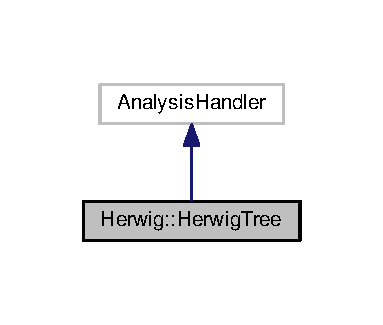
\includegraphics[width=184pt]{class_herwig_1_1_herwig_tree__inherit__graph}
\end{center}
\end{figure}


Collaboration diagram for Herwig\+:\+:Herwig\+Tree\+:\nopagebreak
\begin{figure}[H]
\begin{center}
\leavevmode
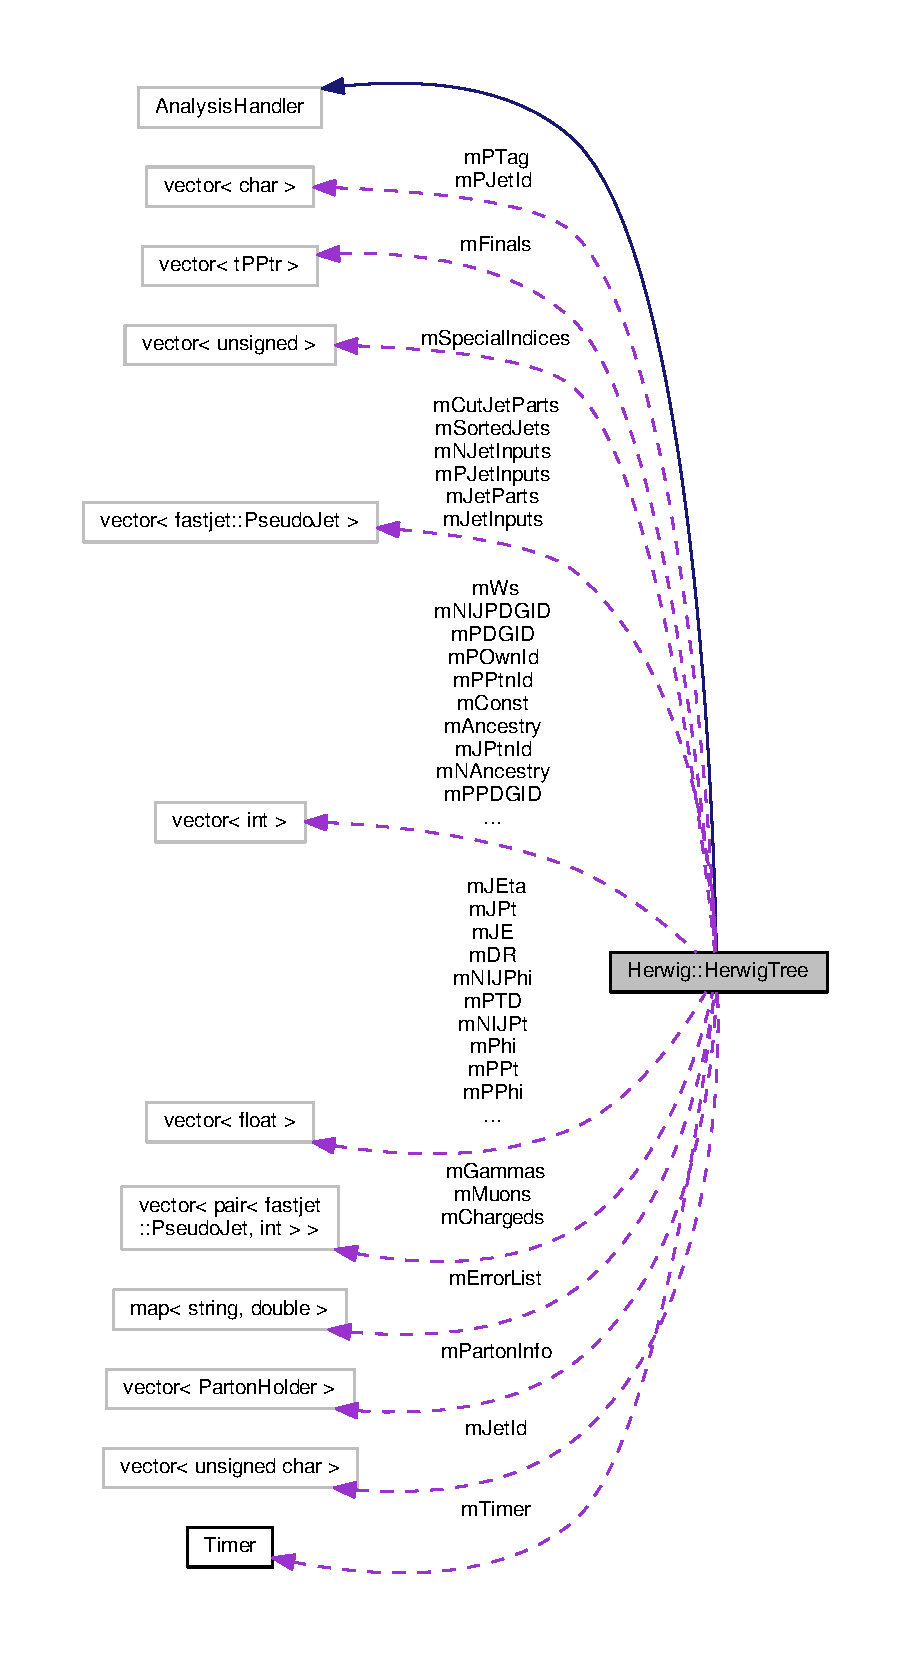
\includegraphics[height=550pt]{class_herwig_1_1_herwig_tree__coll__graph}
\end{center}
\end{figure}
\subsection*{Protected Member Functions}
\begin{Indent}{\bf Standard logistics.}\par
\begin{DoxyCompactItemize}
\item 
virtual I\+B\+Ptr \hyperlink{class_herwig_1_1_herwig_tree_a942f95b5dbcd02b014541a79f8fa5eb3}{clone} () const 
\item 
virtual I\+B\+Ptr \hyperlink{class_herwig_1_1_herwig_tree_a380c78ab7f8c7486d9a356ab4af2fa87}{fullclone} () const 
\item 
virtual void \hyperlink{class_herwig_1_1_herwig_tree_ad6dce6737790c0e08f0f74b304f875ad}{doinitrun} ()
\item 
virtual void \hyperlink{class_herwig_1_1_herwig_tree_aa520a60f4bd7dc79f514eb03156cbb5b}{dofinish} ()
\end{DoxyCompactItemize}
\end{Indent}
\begin{Indent}{\bf Fragmentation of the analysis chain.}\par
\begin{DoxyCompactItemize}
\item 
void \hyperlink{class_herwig_1_1_herwig_tree_a15241d3c3022e5adc42b6d14a58db793}{Initialize} ()
\item 
bool \hyperlink{class_herwig_1_1_herwig_tree_aaff97a85da1095113b8a9c9cea55f504}{Hard\+Proc} ()
\item 
bool \hyperlink{class_herwig_1_1_herwig_tree_abecfba3d8edb2d977782e980fdf5cdd5}{Final\+State} ()
\item 
bool \hyperlink{class_herwig_1_1_herwig_tree_a5841f99ecb35a9eedf9c87e8c217cd63}{Jet\+Loop} ()
\item 
bool \hyperlink{class_herwig_1_1_herwig_tree_a5c00e67d9cfde9db3b3f78a1d71fc43b}{Isolation\+Proc} ()
\item 
bool \hyperlink{class_herwig_1_1_herwig_tree_aff911b963152c83b2825f7d2f7ca6817}{Isolation\+Photons} (int iprt, fastjet\+::\+Pseudo\+Jet \&ipart)
\item 
bool \hyperlink{class_herwig_1_1_herwig_tree_af5641afa4dfabbd045e5e79b3ffe6bdb}{Isolation\+Muons} (int iprt, fastjet\+::\+Pseudo\+Jet \&ipart)
\item 
bool \hyperlink{class_herwig_1_1_herwig_tree_a150ce42e768874f6769f0dfca78865a2}{Isolation\+Leptons} (int iprt, fastjet\+::\+Pseudo\+Jet \&ipart)
\item 
bool \hyperlink{class_herwig_1_1_herwig_tree_a2151de137082d50455c75409d0ea3901}{Isolation\+From\+Jets} ()
\end{DoxyCompactItemize}
\end{Indent}
\begin{Indent}{\bf Event-\/type specific analysis actions.}\par
\begin{DoxyCompactItemize}
\item 
bool \hyperlink{class_herwig_1_1_herwig_tree_a55907713e973e992e7156a76852843b1}{Gamma\+Add} (t\+P\+Ptr gamma)
\item 
bool \hyperlink{class_herwig_1_1_herwig_tree_a1d5bb682934cefecc178353febce65fc}{Muon\+Add} (t\+P\+Ptr muon)
\item 
bool \hyperlink{class_herwig_1_1_herwig_tree_a16313dcbb3bbdd10712e175688e76786}{Lepton\+Add} (t\+P\+Ptr lepton, int parent=-\/1)
\end{DoxyCompactItemize}
\end{Indent}
\begin{Indent}{\bf Helper methods for the analysis}\par
\begin{DoxyCompactItemize}
\item 
void \hyperlink{class_herwig_1_1_herwig_tree_aff2fb52aa58050f06ef3e4348dc212b5}{B\+Neutrinos} (const t\+P\+Ptr \&part)
\item 
int \hyperlink{class_herwig_1_1_herwig_tree_a53035783c31d12776ea6410765fbc82c}{Get\+Status\+Code} (const t\+P\+Ptr \&part) const 
\item 
bool \hyperlink{class_herwig_1_1_herwig_tree_a4bbe10f94b263debf418806437eb12c7}{Gamma\+Checker} (const t\+P\+Ptr \&gamma) const 
\item 
int \hyperlink{class_herwig_1_1_herwig_tree_a857bd97b8e91ebef6e7c82b0cc3117b0}{Is\+Excited\+Hadron\+State} (const t\+P\+Ptr \&part, int quark\+Id) const 
\item 
void \hyperlink{class_herwig_1_1_herwig_tree_a227e5340755c44ba4cf624db61ca1ca1}{Repeat} ()
\end{DoxyCompactItemize}
\end{Indent}
\begin{Indent}{\bf Functions for adding stuff to be saved}\par
\begin{DoxyCompactItemize}
\item 
void \hyperlink{class_herwig_1_1_herwig_tree_a5d32e316c3369a0b9832689c93c4def6}{Particle\+Add} (const t\+P\+Ptr \&part, char jetid)
\item 
void \hyperlink{class_herwig_1_1_herwig_tree_ae03124197c64e55ae4ff6b63b8b15065}{Parton\+Add} (const t\+P\+Ptr \&part, char jetid, char tag, int ptnid=-\/1, int ownid=-\/1)
\item 
void \hyperlink{class_herwig_1_1_herwig_tree_a4aa2bfe3825370d30304afee49896c7a}{Parton\+Add} (unsigned num, char jetid)
\item 
void \hyperlink{class_herwig_1_1_herwig_tree_a0487de1b58e25fd5ca561ee4304256b3}{Jet\+Add} (unsigned jet, int spoil=0)
\item 
void \hyperlink{class_herwig_1_1_herwig_tree_a6a6b0cb9f7b1870cc55895f182b974c1}{Parton\+Append} (fastjet\+::\+Pseudo\+Jet p4, t\+P\+Ptr part, char tag, int ptnid=-\/1)
\end{DoxyCompactItemize}
\end{Indent}
\begin{Indent}{\bf Miscellaneous helper functions}\par
\begin{DoxyCompactItemize}
\item 
void \hyperlink{class_herwig_1_1_herwig_tree_aeb56d225d324365a52789a1949a6452b}{Cuts} ()
\item 
double \hyperlink{class_herwig_1_1_herwig_tree_a153d67d1f7a9e992906e7159636d5f2b}{P\+TD} ()
\item 
double \hyperlink{class_herwig_1_1_herwig_tree_a4907ce27ad1397dc907c7a1c34307ecb}{Sigma2} ()
\item 
bool \hyperlink{class_herwig_1_1_herwig_tree_ac9d8b482bcf0533674bd6d6d1be099d1}{Is\+Charged} (int pdgid) const 
\item 
bool \hyperlink{class_herwig_1_1_herwig_tree_ae34cc1baf995effda3cdefac42e919cb}{Is\+Hadron} (int pdgid) const 
\item 
bool \hyperlink{class_herwig_1_1_herwig_tree_adbb3787d260f0e607ddc416d3ede25a1}{Is\+Parton} (int pdgid) const 
\item 
bool \hyperlink{class_herwig_1_1_herwig_tree_a66916f6b6b836a0fb1f824c2072051c2}{Is\+Lepton} (int pdgid) const 
\item 
void \hyperlink{class_herwig_1_1_herwig_tree_a7b26f690399e3b09a3a932914b2ee004}{Parton\+Descend} (t\+P\+Ptr part)
\item 
t\+P\+Ptr \hyperlink{class_herwig_1_1_herwig_tree_a4f813c334d7580baaf3ff5bc09ab4ba7}{Optimal\+Parton} (t\+P\+Ptr part) const 
\item 
Lorentz5\+Momentum \hyperlink{class_herwig_1_1_herwig_tree_a62fdf42b0dea6df4c413a443febdd5d7}{Final\+Momenta} (t\+P\+Ptr parent) const 
\item 
Lorentz5\+Momentum \hyperlink{class_herwig_1_1_herwig_tree_a6860912cfb61e8e17b039ee8a03eabc7}{Final\+P\+Momenta} (t\+P\+Ptr parent) const 
\item 
void \hyperlink{class_herwig_1_1_herwig_tree_a1879d8a4e4b59c7ce1ca8d667bc2ee75}{Print\+\_\+parents} (const t\+P\+Ptr \&part) const 
\item 
void \hyperlink{class_herwig_1_1_herwig_tree_ae41aeb0678da062374c772796f990c92}{Iter\+\_\+print} (t\+P\+Ptr part, unsigned gen) const 
\item 
bool \hyperlink{class_herwig_1_1_herwig_tree_ab962acb7d1acbdd99aacfaaf6a2c3c04}{Absent} (unsigned int num) const 
\item 
void \hyperlink{class_herwig_1_1_herwig_tree_aff161fa1b8517b8e28eec5b845a987e6}{Add\+Message} (string msg, double wgt)
\item 
T\+Lorentz\+Vector \hyperlink{class_herwig_1_1_herwig_tree_a07d4fcc254706e8380c47a30bcc8f303}{T\+Lorentzify} (const t\+P\+Ptr \&part) const 
\item 
fastjet\+::\+Pseudo\+Jet \hyperlink{class_herwig_1_1_herwig_tree_a9d29816b401eaf3746db1c91f8d03549}{Pseudo\+Jettify} (const t\+P\+Ptr \&part) const 
\item 
fastjet\+::\+Pseudo\+Jet \hyperlink{class_herwig_1_1_herwig_tree_a8941cb1d95ce44bad9f88e24004b666b}{Pseudo\+Jettify} (T\+Lorentz\+Vector p4) const 
\end{DoxyCompactItemize}
\end{Indent}
\subsection*{Protected Attributes}
\begin{DoxyCompactItemize}
\item 
vector$<$ char $>$ \hyperlink{class_herwig_1_1_herwig_tree_a2959f5c6970dffaa74eeb606c650b04f}{m\+P\+Jet\+Id}
\item 
vector$<$ int $>$ \hyperlink{class_herwig_1_1_herwig_tree_a7dfcff3430486ec5f022b2ecce0ee62f}{m\+P\+Ptn\+Id}
\item 
vector$<$ int $>$ \hyperlink{class_herwig_1_1_herwig_tree_a11a7a3ded9e4268d2a1152e48de1c761}{m\+P\+Own\+Id}
\item 
vector$<$ int $>$ \hyperlink{class_herwig_1_1_herwig_tree_ac0b628d7f65f0dd5282a6f37ed75cd62}{m\+P\+P\+D\+G\+ID}
\item 
vector$<$ char $>$ \hyperlink{class_herwig_1_1_herwig_tree_ad3e9614afd7e68fee47bc102067d3a15}{m\+P\+Tag}
\item 
vector$<$ float $>$ \hyperlink{class_herwig_1_1_herwig_tree_a7097209613587b2065e46044fe3e0dcf}{m\+P\+Pt}
\item 
vector$<$ float $>$ \hyperlink{class_herwig_1_1_herwig_tree_ab79e875b02024eb96d625b32a9e8943e}{m\+P\+Eta}
\item 
vector$<$ float $>$ \hyperlink{class_herwig_1_1_herwig_tree_afd0e29eb67ff06d6325fc5773bcb7d96}{m\+P\+Phi}
\item 
vector$<$ float $>$ \hyperlink{class_herwig_1_1_herwig_tree_a1e002df7309a0a1cb10eae3b807e2d33}{m\+PE}
\item 
vector$<$ float $>$ \hyperlink{class_herwig_1_1_herwig_tree_a68f88a82fd213cbe59b51c019f5773d1}{m\+DR}
\item 
vector$<$ float $>$ \hyperlink{class_herwig_1_1_herwig_tree_ae26408eb10df0fc5643022ea718b73ba}{m\+J\+Pt}
\item 
vector$<$ float $>$ \hyperlink{class_herwig_1_1_herwig_tree_a50b89cfc9ac1d0a0d210483ec0b33584}{m\+J\+Eta}
\item 
vector$<$ float $>$ \hyperlink{class_herwig_1_1_herwig_tree_ae5fb619ee4d7c58f7f6d71d99392dd5b}{m\+J\+Phi}
\item 
vector$<$ float $>$ \hyperlink{class_herwig_1_1_herwig_tree_a49f4d5832d02c8e2e317ffb11c4f4f98}{m\+JE}
\item 
vector$<$ int $>$ \hyperlink{class_herwig_1_1_herwig_tree_aae0a968baf348f5b1b34c0eae9225042}{m\+J\+Ptn\+Id}
\item 
vector$<$ int $>$ \hyperlink{class_herwig_1_1_herwig_tree_a98e0a308cd96f540d32c4f4f21744a97}{m\+Const}
\item 
vector$<$ float $>$ \hyperlink{class_herwig_1_1_herwig_tree_a7b7332a3ca42994d5f044a8edeadeeb2}{m\+P\+TD}
\item 
vector$<$ float $>$ \hyperlink{class_herwig_1_1_herwig_tree_ae4570b94630f03dedd19fd68494b6a71}{m\+Sigma2}
\item 
float \hyperlink{class_herwig_1_1_herwig_tree_a24471be817f37cd3f4f9eb2b984c9260}{m\+Met}
\item 
fastjet\+::\+Pseudo\+Jet \hyperlink{class_herwig_1_1_herwig_tree_a49d3c642cc2d55ee2d96dd063ad8f0ed}{m\+Met\+Vect}
\item 
vector$<$ \hyperlink{struct_parton_holder}{Parton\+Holder} $>$ \hyperlink{class_herwig_1_1_herwig_tree_aea4b92ced12093c2e65c97bfe3a0a839}{m\+Parton\+Info}
\item 
fastjet\+::\+Jet\+Definition\+::\+Plugin $\ast$ \hyperlink{class_herwig_1_1_herwig_tree_a0ca52a2a08bedfe7c516f3efd133d489}{m\+Plugin}
\item 
fastjet\+::\+Jet\+Definition \hyperlink{class_herwig_1_1_herwig_tree_ae80b94db0009e26c4b5fbbc0d14d31b3}{m\+Jet\+Def}
\item 
vector$<$ fastjet\+::\+Pseudo\+Jet $>$ \hyperlink{class_herwig_1_1_herwig_tree_a22ebbb6eef9ef80f746f683008abb301}{m\+Jet\+Inputs}
\item 
vector$<$ fastjet\+::\+Pseudo\+Jet $>$ \hyperlink{class_herwig_1_1_herwig_tree_a217545505d0f79dc889d212ee8f82516}{m\+N\+Jet\+Inputs}
\item 
vector$<$ fastjet\+::\+Pseudo\+Jet $>$ \hyperlink{class_herwig_1_1_herwig_tree_a595863c9ae182137ddaab450045c50a6}{m\+P\+Jet\+Inputs}
\item 
vector$<$ fastjet\+::\+Pseudo\+Jet $>$ \hyperlink{class_herwig_1_1_herwig_tree_a2d63c5091aefdf707d992bd80830e76b}{m\+Sorted\+Jets}
\item 
vector$<$ fastjet\+::\+Pseudo\+Jet $>$ \hyperlink{class_herwig_1_1_herwig_tree_a19bee8df38df5b5fffd77dd75d4ae956}{m\+Jet\+Parts}
\item 
vector$<$ fastjet\+::\+Pseudo\+Jet $>$ \hyperlink{class_herwig_1_1_herwig_tree_a33c5453b6426268754d1f0c36bd62ef1}{m\+Cut\+Jet\+Parts}
\item 
vector$<$ int $>$ \hyperlink{class_herwig_1_1_herwig_tree_a36b5a22cf3dac0687b42e4ee1650aab5}{m\+Ancestry}
\item 
vector$<$ int $>$ \hyperlink{class_herwig_1_1_herwig_tree_aee9127c2468fe19ec48667cd8f3de2a2}{m\+N\+Ancestry}
\item 
vector$<$ int $>$ \hyperlink{class_herwig_1_1_herwig_tree_a19bd4f1ed5bc10ff4523cf3f8120b670}{m\+Ws}
\item 
double \hyperlink{class_herwig_1_1_herwig_tree_a60ae5fcc1fff4256bdd35074035e6a32}{m\+Tot\+Wgt}
\item 
double \hyperlink{class_herwig_1_1_herwig_tree_a2d1cb6fc4a481866ede3796640f05e87}{m\+Sel\+Wgt}
\item 
map$<$ string, double $>$ \hyperlink{class_herwig_1_1_herwig_tree_aa58f96f1caffd3e013d2f341de98bf28}{m\+Error\+List}
\item 
unsigned \hyperlink{class_herwig_1_1_herwig_tree_a211506013383c5057459219813924383}{m\+Hard\+Proc\+Count}
\item 
unsigned \hyperlink{class_herwig_1_1_herwig_tree_aff68962320b3b854debe9db4d52d076a}{m\+Counter}
\item 
int \hyperlink{class_herwig_1_1_herwig_tree_a3dc3453c672a72bce7ca90d9216e7df8}{m\+Lepton\+Friend}
\end{DoxyCompactItemize}
\begin{Indent}{\bf Variables for the analysis}\par
\begin{DoxyCompactItemize}
\item 
t\+Event\+Ptr \hyperlink{class_herwig_1_1_herwig_tree_af603e5812ed44d611aeaa66e7f6616f6}{m\+Event}
\item 
tc\+Event\+Base\+Ptr \hyperlink{class_herwig_1_1_herwig_tree_a96e103a607ddc543e5ad1c4c097da79f}{m\+Hard\+Handler}
\item 
vector$<$ t\+P\+Ptr $>$ \hyperlink{class_herwig_1_1_herwig_tree_abd8e1116b0df9d4214f77ce86438d4d4}{m\+Finals}
\item 
T\+File $\ast$ \hyperlink{class_herwig_1_1_herwig_tree_a8a5667ccbf263bd6e99590b5155d2c46}{m\+File}
\item 
T\+Tree $\ast$ \hyperlink{class_herwig_1_1_herwig_tree_a03788321f05cfb5f7a119beafbaa29d4}{m\+Tree}
\item 
int \hyperlink{class_herwig_1_1_herwig_tree_a170499fc649b5aced8f83adc5bf8c914}{m\+Num\+Events}
\item 
int \hyperlink{class_herwig_1_1_herwig_tree_a1d47a9344b42319950182483f08444d1}{m\+Mode}
\item 
int \hyperlink{class_herwig_1_1_herwig_tree_a52f0f5dff398cec2740c10dd095f50ec}{m\+Timer\+Step}
\item 
\hyperlink{class_timer}{Timer} \hyperlink{class_herwig_1_1_herwig_tree_a72fcb4b6832d4782d0096c4a16a16683}{m\+Timer}
\item 
vector$<$ unsigned $>$ \hyperlink{class_herwig_1_1_herwig_tree_aa1b6f46c32e4d9ccf20dce2515cfd1e7}{m\+Special\+Indices}
\item 
char \hyperlink{class_herwig_1_1_herwig_tree_a3a3a0ddaf489eb0e4a049eaf7cd084b2}{m\+B\+Nu\+Count}
\item 
char \hyperlink{class_herwig_1_1_herwig_tree_a28df6b8b7b033370f9817f3e055fbb44}{m\+O\+Nu\+Count}
\item 
char \hyperlink{class_herwig_1_1_herwig_tree_a25e21e2c469c2a038390355a95423b83}{m\+Nu\+OB}
\item 
char \hyperlink{class_herwig_1_1_herwig_tree_a65ef841ae6a9c77c5a351349a26d3005}{m\+Nu\+OC}
\item 
char \hyperlink{class_herwig_1_1_herwig_tree_a68bc0ced9a248641fa1448a2d4fcc5b6}{m\+Nu\+O\+Lept}
\item 
char \hyperlink{class_herwig_1_1_herwig_tree_a602e6fb6d9510a1b4bd75d39b3995aa2}{m\+Nu\+O\+Other}
\item 
char \hyperlink{class_herwig_1_1_herwig_tree_acd4aa13b4a8936a89173fbb63ed161e8}{m\+NuB}
\item 
char \hyperlink{class_herwig_1_1_herwig_tree_a640d1260f445fbb7149fedc432319dfd}{m\+NuC}
\item 
char \hyperlink{class_herwig_1_1_herwig_tree_a70de329a4eda6e336b1a6154562e2637}{m\+Nu\+Lept}
\item 
char \hyperlink{class_herwig_1_1_herwig_tree_ab2546c8d2a180686b60c56dab084f90e}{m\+Nu\+Other}
\item 
char \hyperlink{class_herwig_1_1_herwig_tree_ac49d274539b787810d87c13984d1679f}{m\+Info}
\item 
float \hyperlink{class_herwig_1_1_herwig_tree_a161ab96ab6f288fcf9ae7da484b690f8}{m\+Weight}
\item 
float \hyperlink{class_herwig_1_1_herwig_tree_ab7d94d7d284990f8512a285a578bb0e5}{m\+Pt\+Hat}
\item 
vector$<$ float $>$ \hyperlink{class_herwig_1_1_herwig_tree_a216647b55088bd7af117564be968e4aa}{m\+Isolation}
\end{DoxyCompactItemize}
\end{Indent}
\begin{Indent}{\bf Particle level for the particles within jets.}\par
\begin{DoxyCompactItemize}
\item 
vector$<$ unsigned char $>$ \hyperlink{class_herwig_1_1_herwig_tree_a2b7790f57e9e3e44cb10747b0bafdaa1}{m\+Jet\+Id}
\item 
vector$<$ int $>$ \hyperlink{class_herwig_1_1_herwig_tree_ab6991935c69e5fb1f0e03e9e8e22fdd6}{m\+P\+D\+G\+ID}
\item 
vector$<$ float $>$ \hyperlink{class_herwig_1_1_herwig_tree_a545def11295a75086186c73aa393e0b4}{m\+Pt}
\item 
vector$<$ float $>$ \hyperlink{class_herwig_1_1_herwig_tree_a16fc9feb3ba75e30c41e3842b0b324af}{m\+Eta}
\item 
vector$<$ float $>$ \hyperlink{class_herwig_1_1_herwig_tree_a9d3ad17856037f6b1d3229ed9086f636}{m\+Phi}
\item 
vector$<$ float $>$ \hyperlink{class_herwig_1_1_herwig_tree_a14b6321a20f27ad9211ad7624113bb3b}{mE}
\item 
vector$<$ int $>$ \hyperlink{class_herwig_1_1_herwig_tree_a6fbb8c1dd6e2b4ed67122f74ab0da929}{m\+N\+I\+J\+P\+D\+G\+ID}
\item 
vector$<$ float $>$ \hyperlink{class_herwig_1_1_herwig_tree_a95e4e19ce467ec60b52960103eadeff7}{m\+N\+I\+J\+Pt}
\item 
vector$<$ float $>$ \hyperlink{class_herwig_1_1_herwig_tree_aef150f8f0a6ace649bb0d794577c6705}{m\+N\+I\+J\+Eta}
\item 
vector$<$ float $>$ \hyperlink{class_herwig_1_1_herwig_tree_a6d02449335894d8aaa1d794c08d18108}{m\+N\+I\+J\+Phi}
\item 
vector$<$ float $>$ \hyperlink{class_herwig_1_1_herwig_tree_a7b03a77b42e5d27533adcbeb6cc6e701}{m\+N\+I\+JE}
\end{DoxyCompactItemize}
\end{Indent}
\begin{Indent}{\bf Containers for objects that are tested for isolation.}\par
\begin{DoxyCompactItemize}
\item 
vector$<$ pair$<$ fastjet\+::\+Pseudo\+Jet, int $>$ $>$ \hyperlink{class_herwig_1_1_herwig_tree_a5cb588d629626d524e56d88b93082d3a}{m\+Gammas}
\item 
vector$<$ pair$<$ fastjet\+::\+Pseudo\+Jet, int $>$ $>$ \hyperlink{class_herwig_1_1_herwig_tree_a9c61c42232484ac6b345ef8720131a5c}{m\+Chargeds}
\item 
vector$<$ pair$<$ fastjet\+::\+Pseudo\+Jet, int $>$ $>$ \hyperlink{class_herwig_1_1_herwig_tree_a03ab2e508845e15bd0967a055d5fc45b}{m\+Muons}
\end{DoxyCompactItemize}
\end{Indent}
\subsection*{Methods visible to the outside.}
\begin{DoxyCompactItemize}
\item 
\hyperlink{class_herwig_1_1_herwig_tree_a02551fe885aebae778e2df85f5f810f6}{Herwig\+Tree} ()
\begin{DoxyCompactList}\small\item\em Constructor does literally nothing. See \hyperlink{class_herwig_1_1_herwig_tree_ad6dce6737790c0e08f0f74b304f875ad}{doinitrun()}. \end{DoxyCompactList}\item 
virtual void \hyperlink{class_herwig_1_1_herwig_tree_ae478dd545ede60f68fdd161d61d74fee}{analyze} (t\+Event\+Ptr event, long ieve, int loop, int state)
\item 
static void \hyperlink{class_herwig_1_1_herwig_tree_a3cd627f436988cb65b02bc6b38c73ccc}{Init} ()
\end{DoxyCompactItemize}


\subsection{Detailed Description}
The main class handle for the Herwig7 analysis. 

Inherits from Analysis\+Handler, and some structures need to follow structures according to this. Our own class methods start with a capital letter and those given by Herwig7 with a lower case letter. 

Definition at line 151 of file Herwig\+Tree.\+h.



\subsection{Constructor \& Destructor Documentation}
\index{Herwig\+::\+Herwig\+Tree@{Herwig\+::\+Herwig\+Tree}!Herwig\+Tree@{Herwig\+Tree}}
\index{Herwig\+Tree@{Herwig\+Tree}!Herwig\+::\+Herwig\+Tree@{Herwig\+::\+Herwig\+Tree}}
\subsubsection[{\texorpdfstring{Herwig\+Tree()}{HerwigTree()}}]{\setlength{\rightskip}{0pt plus 5cm}Herwig\+::\+Herwig\+Tree\+::\+Herwig\+Tree (
\begin{DoxyParamCaption}
{}
\end{DoxyParamCaption}
)\hspace{0.3cm}{\ttfamily [inline]}}\hypertarget{class_herwig_1_1_herwig_tree_a02551fe885aebae778e2df85f5f810f6}{}\label{class_herwig_1_1_herwig_tree_a02551fe885aebae778e2df85f5f810f6}


Constructor does literally nothing. See \hyperlink{class_herwig_1_1_herwig_tree_ad6dce6737790c0e08f0f74b304f875ad}{doinitrun()}. 



Definition at line 157 of file Herwig\+Tree.\+h.



\subsection{Member Function Documentation}
\index{Herwig\+::\+Herwig\+Tree@{Herwig\+::\+Herwig\+Tree}!Absent@{Absent}}
\index{Absent@{Absent}!Herwig\+::\+Herwig\+Tree@{Herwig\+::\+Herwig\+Tree}}
\subsubsection[{\texorpdfstring{Absent(unsigned int num) const }{Absent(unsigned int num) const }}]{\setlength{\rightskip}{0pt plus 5cm}bool Herwig\+Tree\+::\+Absent (
\begin{DoxyParamCaption}
\item[{unsigned int}]{num}
\end{DoxyParamCaption}
) const\hspace{0.3cm}{\ttfamily [inline]}, {\ttfamily [protected]}}\hypertarget{class_herwig_1_1_herwig_tree_ab962acb7d1acbdd99aacfaaf6a2c3c04}{}\label{class_herwig_1_1_herwig_tree_ab962acb7d1acbdd99aacfaaf6a2c3c04}
Is the given value absent from m\+Special\+Indices? 
\begin{DoxyParams}{Parameters}
{\em num} & The current particle number. \\
\hline
\end{DoxyParams}


Definition at line 1078 of file Herwig\+Tree.\+cpp.

\index{Herwig\+::\+Herwig\+Tree@{Herwig\+::\+Herwig\+Tree}!Add\+Message@{Add\+Message}}
\index{Add\+Message@{Add\+Message}!Herwig\+::\+Herwig\+Tree@{Herwig\+::\+Herwig\+Tree}}
\subsubsection[{\texorpdfstring{Add\+Message(string msg, double wgt)}{AddMessage(string msg, double wgt)}}]{\setlength{\rightskip}{0pt plus 5cm}void Herwig\+Tree\+::\+Add\+Message (
\begin{DoxyParamCaption}
\item[{string}]{msg, }
\item[{double}]{wgt}
\end{DoxyParamCaption}
)\hspace{0.3cm}{\ttfamily [inline]}, {\ttfamily [protected]}}\hypertarget{class_herwig_1_1_herwig_tree_aff161fa1b8517b8e28eec5b845a987e6}{}\label{class_herwig_1_1_herwig_tree_aff161fa1b8517b8e28eec5b845a987e6}
Problems in the creation. 
\begin{DoxyParams}{Parameters}
{\em msg} & The \char`\"{}problem\char`\"{}. \\
\hline
{\em wgt} & The current event weight. \\
\hline
\end{DoxyParams}


Definition at line 1083 of file Herwig\+Tree.\+cpp.

\index{Herwig\+::\+Herwig\+Tree@{Herwig\+::\+Herwig\+Tree}!analyze@{analyze}}
\index{analyze@{analyze}!Herwig\+::\+Herwig\+Tree@{Herwig\+::\+Herwig\+Tree}}
\subsubsection[{\texorpdfstring{analyze(t\+Event\+Ptr event, long ieve, int loop, int state)}{analyze(tEventPtr event, long ieve, int loop, int state)}}]{\setlength{\rightskip}{0pt plus 5cm}void Herwig\+Tree\+::analyze (
\begin{DoxyParamCaption}
\item[{t\+Event\+Ptr}]{event, }
\item[{long}]{ieve, }
\item[{int}]{loop, }
\item[{int}]{state}
\end{DoxyParamCaption}
)\hspace{0.3cm}{\ttfamily [virtual]}}\hypertarget{class_herwig_1_1_herwig_tree_ae478dd545ede60f68fdd161d61d74fee}{}\label{class_herwig_1_1_herwig_tree_ae478dd545ede60f68fdd161d61d74fee}
Analyze a given Event. 
\begin{DoxyParams}{Parameters}
{\em event} & Pointer to the Event to be analyzed. \\
\hline
{\em ieve} & The event number. \\
\hline
{\em loop} & The number of times this event has been presented. \\
\hline
{\em state} & Nonzero if the event has been manipulated. \\
\hline
\end{DoxyParams}


Definition at line 169 of file Herwig\+Tree.\+cpp.

\index{Herwig\+::\+Herwig\+Tree@{Herwig\+::\+Herwig\+Tree}!B\+Neutrinos@{B\+Neutrinos}}
\index{B\+Neutrinos@{B\+Neutrinos}!Herwig\+::\+Herwig\+Tree@{Herwig\+::\+Herwig\+Tree}}
\subsubsection[{\texorpdfstring{B\+Neutrinos(const t\+P\+Ptr \&part)}{BNeutrinos(const tPPtr &part)}}]{\setlength{\rightskip}{0pt plus 5cm}void Herwig\+::\+Herwig\+Tree\+::\+B\+Neutrinos (
\begin{DoxyParamCaption}
\item[{const t\+P\+Ptr \&}]{part}
\end{DoxyParamCaption}
)\hspace{0.3cm}{\ttfamily [protected]}}\hypertarget{class_herwig_1_1_herwig_tree_aff2fb52aa58050f06ef3e4348dc212b5}{}\label{class_herwig_1_1_herwig_tree_aff2fb52aa58050f06ef3e4348dc212b5}
A function for finding b neutrinos 
\begin{DoxyParams}{Parameters}
{\em parrt} & The b-\/parton to study. \\
\hline
\end{DoxyParams}


Definition at line 813 of file Herwig\+Tree.\+cpp.

\index{Herwig\+::\+Herwig\+Tree@{Herwig\+::\+Herwig\+Tree}!clone@{clone}}
\index{clone@{clone}!Herwig\+::\+Herwig\+Tree@{Herwig\+::\+Herwig\+Tree}}
\subsubsection[{\texorpdfstring{clone() const }{clone() const }}]{\setlength{\rightskip}{0pt plus 5cm}virtual I\+B\+Ptr Herwig\+::\+Herwig\+Tree\+::clone (
\begin{DoxyParamCaption}
{}
\end{DoxyParamCaption}
) const\hspace{0.3cm}{\ttfamily [inline]}, {\ttfamily [protected]}, {\ttfamily [virtual]}}\hypertarget{class_herwig_1_1_herwig_tree_a942f95b5dbcd02b014541a79f8fa5eb3}{}\label{class_herwig_1_1_herwig_tree_a942f95b5dbcd02b014541a79f8fa5eb3}


Definition at line 173 of file Herwig\+Tree.\+h.

\index{Herwig\+::\+Herwig\+Tree@{Herwig\+::\+Herwig\+Tree}!Cuts@{Cuts}}
\index{Cuts@{Cuts}!Herwig\+::\+Herwig\+Tree@{Herwig\+::\+Herwig\+Tree}}
\subsubsection[{\texorpdfstring{Cuts()}{Cuts()}}]{\setlength{\rightskip}{0pt plus 5cm}void Herwig\+Tree\+::\+Cuts (
\begin{DoxyParamCaption}
{}
\end{DoxyParamCaption}
)\hspace{0.3cm}{\ttfamily [protected]}}\hypertarget{class_herwig_1_1_herwig_tree_aeb56d225d324365a52789a1949a6452b}{}\label{class_herwig_1_1_herwig_tree_aeb56d225d324365a52789a1949a6452b}
Cuts for jet property calculations. 

Definition at line 942 of file Herwig\+Tree.\+cpp.

\index{Herwig\+::\+Herwig\+Tree@{Herwig\+::\+Herwig\+Tree}!dofinish@{dofinish}}
\index{dofinish@{dofinish}!Herwig\+::\+Herwig\+Tree@{Herwig\+::\+Herwig\+Tree}}
\subsubsection[{\texorpdfstring{dofinish()}{dofinish()}}]{\setlength{\rightskip}{0pt plus 5cm}void Herwig\+::\+Herwig\+Tree\+::dofinish (
\begin{DoxyParamCaption}
{}
\end{DoxyParamCaption}
)\hspace{0.3cm}{\ttfamily [inline]}, {\ttfamily [protected]}, {\ttfamily [virtual]}}\hypertarget{class_herwig_1_1_herwig_tree_aa520a60f4bd7dc79f514eb03156cbb5b}{}\label{class_herwig_1_1_herwig_tree_aa520a60f4bd7dc79f514eb03156cbb5b}
Finishing (close files etc.).

Operations to be performed as the run is finished. 

Definition at line 599 of file Herwig\+Tree.\+h.

\index{Herwig\+::\+Herwig\+Tree@{Herwig\+::\+Herwig\+Tree}!doinitrun@{doinitrun}}
\index{doinitrun@{doinitrun}!Herwig\+::\+Herwig\+Tree@{Herwig\+::\+Herwig\+Tree}}
\subsubsection[{\texorpdfstring{doinitrun()}{doinitrun()}}]{\setlength{\rightskip}{0pt plus 5cm}void Herwig\+::\+Herwig\+Tree\+::doinitrun (
\begin{DoxyParamCaption}
{}
\end{DoxyParamCaption}
)\hspace{0.3cm}{\ttfamily [inline]}, {\ttfamily [protected]}, {\ttfamily [virtual]}}\hypertarget{class_herwig_1_1_herwig_tree_ad6dce6737790c0e08f0f74b304f875ad}{}\label{class_herwig_1_1_herwig_tree_ad6dce6737790c0e08f0f74b304f875ad}
Initialization (open files etc.). Connect an event handle with the tree 

Definition at line 467 of file Herwig\+Tree.\+h.

\index{Herwig\+::\+Herwig\+Tree@{Herwig\+::\+Herwig\+Tree}!Final\+Momenta@{Final\+Momenta}}
\index{Final\+Momenta@{Final\+Momenta}!Herwig\+::\+Herwig\+Tree@{Herwig\+::\+Herwig\+Tree}}
\subsubsection[{\texorpdfstring{Final\+Momenta(t\+P\+Ptr parent) const }{FinalMomenta(tPPtr parent) const }}]{\setlength{\rightskip}{0pt plus 5cm}Lorentz5\+Momentum Herwig\+Tree\+::\+Final\+Momenta (
\begin{DoxyParamCaption}
\item[{t\+P\+Ptr}]{parent}
\end{DoxyParamCaption}
) const\hspace{0.3cm}{\ttfamily [protected]}}\hypertarget{class_herwig_1_1_herwig_tree_a62fdf42b0dea6df4c413a443febdd5d7}{}\label{class_herwig_1_1_herwig_tree_a62fdf42b0dea6df4c413a443febdd5d7}
Calculate corrected momentum from final-\/state descendants. 
\begin{DoxyParams}{Parameters}
{\em psum} & The value of the momentum sum. \\
\hline
{\em parent} & The current parent to study. \\
\hline
\end{DoxyParams}


Definition at line 871 of file Herwig\+Tree.\+cpp.

\index{Herwig\+::\+Herwig\+Tree@{Herwig\+::\+Herwig\+Tree}!Final\+P\+Momenta@{Final\+P\+Momenta}}
\index{Final\+P\+Momenta@{Final\+P\+Momenta}!Herwig\+::\+Herwig\+Tree@{Herwig\+::\+Herwig\+Tree}}
\subsubsection[{\texorpdfstring{Final\+P\+Momenta(t\+P\+Ptr parent) const }{FinalPMomenta(tPPtr parent) const }}]{\setlength{\rightskip}{0pt plus 5cm}Lorentz5\+Momentum Herwig\+Tree\+::\+Final\+P\+Momenta (
\begin{DoxyParamCaption}
\item[{t\+P\+Ptr}]{parent}
\end{DoxyParamCaption}
) const\hspace{0.3cm}{\ttfamily [protected]}}\hypertarget{class_herwig_1_1_herwig_tree_a6860912cfb61e8e17b039ee8a03eabc7}{}\label{class_herwig_1_1_herwig_tree_a6860912cfb61e8e17b039ee8a03eabc7}
Calculate corrected momentum from final-\/state parton descendants. 
\begin{DoxyParams}{Parameters}
{\em psum} & The value of the momentum sum. \\
\hline
{\em parent} & The current parent to study. \\
\hline
\end{DoxyParams}


Definition at line 882 of file Herwig\+Tree.\+cpp.

\index{Herwig\+::\+Herwig\+Tree@{Herwig\+::\+Herwig\+Tree}!Final\+State@{Final\+State}}
\index{Final\+State@{Final\+State}!Herwig\+::\+Herwig\+Tree@{Herwig\+::\+Herwig\+Tree}}
\subsubsection[{\texorpdfstring{Final\+State()}{FinalState()}}]{\setlength{\rightskip}{0pt plus 5cm}bool Herwig\+Tree\+::\+Final\+State (
\begin{DoxyParamCaption}
{}
\end{DoxyParamCaption}
)\hspace{0.3cm}{\ttfamily [protected]}}\hypertarget{class_herwig_1_1_herwig_tree_abecfba3d8edb2d977782e980fdf5cdd5}{}\label{class_herwig_1_1_herwig_tree_abecfba3d8edb2d977782e980fdf5cdd5}
Analyze the final state. \begin{DoxyReturn}{Returns}
true if the final state is good, false otherwise. 
\end{DoxyReturn}


Definition at line 402 of file Herwig\+Tree.\+cpp.

\index{Herwig\+::\+Herwig\+Tree@{Herwig\+::\+Herwig\+Tree}!fullclone@{fullclone}}
\index{fullclone@{fullclone}!Herwig\+::\+Herwig\+Tree@{Herwig\+::\+Herwig\+Tree}}
\subsubsection[{\texorpdfstring{fullclone() const }{fullclone() const }}]{\setlength{\rightskip}{0pt plus 5cm}virtual I\+B\+Ptr Herwig\+::\+Herwig\+Tree\+::fullclone (
\begin{DoxyParamCaption}
{}
\end{DoxyParamCaption}
) const\hspace{0.3cm}{\ttfamily [inline]}, {\ttfamily [protected]}, {\ttfamily [virtual]}}\hypertarget{class_herwig_1_1_herwig_tree_a380c78ab7f8c7486d9a356ab4af2fa87}{}\label{class_herwig_1_1_herwig_tree_a380c78ab7f8c7486d9a356ab4af2fa87}


Definition at line 174 of file Herwig\+Tree.\+h.

\index{Herwig\+::\+Herwig\+Tree@{Herwig\+::\+Herwig\+Tree}!Gamma\+Add@{Gamma\+Add}}
\index{Gamma\+Add@{Gamma\+Add}!Herwig\+::\+Herwig\+Tree@{Herwig\+::\+Herwig\+Tree}}
\subsubsection[{\texorpdfstring{Gamma\+Add(t\+P\+Ptr gamma)}{GammaAdd(tPPtr gamma)}}]{\setlength{\rightskip}{0pt plus 5cm}bool Herwig\+Tree\+::\+Gamma\+Add (
\begin{DoxyParamCaption}
\item[{t\+P\+Ptr}]{gamma}
\end{DoxyParamCaption}
)\hspace{0.3cm}{\ttfamily [protected]}}\hypertarget{class_herwig_1_1_herwig_tree_a55907713e973e992e7156a76852843b1}{}\label{class_herwig_1_1_herwig_tree_a55907713e973e992e7156a76852843b1}
Add a photon in a gamma+jets event. 
\begin{DoxyParams}{Parameters}
{\em gamma} & The signal photon. \\
\hline
\end{DoxyParams}


Definition at line 694 of file Herwig\+Tree.\+cpp.

\index{Herwig\+::\+Herwig\+Tree@{Herwig\+::\+Herwig\+Tree}!Gamma\+Checker@{Gamma\+Checker}}
\index{Gamma\+Checker@{Gamma\+Checker}!Herwig\+::\+Herwig\+Tree@{Herwig\+::\+Herwig\+Tree}}
\subsubsection[{\texorpdfstring{Gamma\+Checker(const t\+P\+Ptr \&gamma) const }{GammaChecker(const tPPtr &gamma) const }}]{\setlength{\rightskip}{0pt plus 5cm}bool Herwig\+Tree\+::\+Gamma\+Checker (
\begin{DoxyParamCaption}
\item[{const t\+P\+Ptr \&}]{gamma}
\end{DoxyParamCaption}
) const\hspace{0.3cm}{\ttfamily [protected]}}\hypertarget{class_herwig_1_1_herwig_tree_a4bbe10f94b263debf418806437eb12c7}{}\label{class_herwig_1_1_herwig_tree_a4bbe10f94b263debf418806437eb12c7}
A function that checks whether a photon is originated from a pi0 and that the energy of the photon-\/pair corresponds to the pion. returns 0 if the origin is not a pion with good energy and 1 if it is. 
\begin{DoxyParams}{Parameters}
{\em gamma} & The photon to study. \\
\hline
\end{DoxyParams}
\begin{DoxyReturn}{Returns}
false if not pi0 photon, otherwise true. 
\end{DoxyReturn}


Definition at line 1023 of file Herwig\+Tree.\+cpp.

\index{Herwig\+::\+Herwig\+Tree@{Herwig\+::\+Herwig\+Tree}!Get\+Status\+Code@{Get\+Status\+Code}}
\index{Get\+Status\+Code@{Get\+Status\+Code}!Herwig\+::\+Herwig\+Tree@{Herwig\+::\+Herwig\+Tree}}
\subsubsection[{\texorpdfstring{Get\+Status\+Code(const t\+P\+Ptr \&part) const }{GetStatusCode(const tPPtr &part) const }}]{\setlength{\rightskip}{0pt plus 5cm}int Herwig\+Tree\+::\+Get\+Status\+Code (
\begin{DoxyParamCaption}
\item[{const t\+P\+Ptr \&}]{part}
\end{DoxyParamCaption}
) const\hspace{0.3cm}{\ttfamily [protected]}}\hypertarget{class_herwig_1_1_herwig_tree_a53035783c31d12776ea6410765fbc82c}{}\label{class_herwig_1_1_herwig_tree_a53035783c31d12776ea6410765fbc82c}
\hyperlink{namespace_the_p_e_g}{The\+P\+EG} does not provide useful status codes and the status has to be studied manually. This method is a mock-\/up of the C\+M\+S\+S\+W-\/way to calculate the status code. 
\begin{DoxyParams}{Parameters}
{\em part} & The particle to study. \\
\hline
\end{DoxyParams}
\begin{DoxyReturn}{Returns}
1 for final state, 2 for intermediate and 3 for unusable intermediate. 
\end{DoxyReturn}


Definition at line 1049 of file Herwig\+Tree.\+cpp.

\index{Herwig\+::\+Herwig\+Tree@{Herwig\+::\+Herwig\+Tree}!Hard\+Proc@{Hard\+Proc}}
\index{Hard\+Proc@{Hard\+Proc}!Herwig\+::\+Herwig\+Tree@{Herwig\+::\+Herwig\+Tree}}
\subsubsection[{\texorpdfstring{Hard\+Proc()}{HardProc()}}]{\setlength{\rightskip}{0pt plus 5cm}bool Herwig\+Tree\+::\+Hard\+Proc (
\begin{DoxyParamCaption}
{}
\end{DoxyParamCaption}
)\hspace{0.3cm}{\ttfamily [protected]}}\hypertarget{class_herwig_1_1_herwig_tree_aaff97a85da1095113b8a9c9cea55f504}{}\label{class_herwig_1_1_herwig_tree_aaff97a85da1095113b8a9c9cea55f504}
Analyze the hard process. \begin{DoxyReturn}{Returns}
true if Hard process is good, false otherwise. 
\end{DoxyReturn}


Definition at line 595 of file Herwig\+Tree.\+cpp.

\index{Herwig\+::\+Herwig\+Tree@{Herwig\+::\+Herwig\+Tree}!Init@{Init}}
\index{Init@{Init}!Herwig\+::\+Herwig\+Tree@{Herwig\+::\+Herwig\+Tree}}
\subsubsection[{\texorpdfstring{Init()}{Init()}}]{\setlength{\rightskip}{0pt plus 5cm}static void Herwig\+::\+Herwig\+Tree\+::\+Init (
\begin{DoxyParamCaption}
{}
\end{DoxyParamCaption}
)\hspace{0.3cm}{\ttfamily [inline]}, {\ttfamily [static]}}\hypertarget{class_herwig_1_1_herwig_tree_a3cd627f436988cb65b02bc6b38c73ccc}{}\label{class_herwig_1_1_herwig_tree_a3cd627f436988cb65b02bc6b38c73ccc}
Standard Init function, called exactly once. 

Definition at line 167 of file Herwig\+Tree.\+h.

\index{Herwig\+::\+Herwig\+Tree@{Herwig\+::\+Herwig\+Tree}!Initialize@{Initialize}}
\index{Initialize@{Initialize}!Herwig\+::\+Herwig\+Tree@{Herwig\+::\+Herwig\+Tree}}
\subsubsection[{\texorpdfstring{Initialize()}{Initialize()}}]{\setlength{\rightskip}{0pt plus 5cm}void Herwig\+Tree\+::\+Initialize (
\begin{DoxyParamCaption}
{}
\end{DoxyParamCaption}
)\hspace{0.3cm}{\ttfamily [protected]}}\hypertarget{class_herwig_1_1_herwig_tree_a15241d3c3022e5adc42b6d14a58db793}{}\label{class_herwig_1_1_herwig_tree_a15241d3c3022e5adc42b6d14a58db793}
Clear storages etc. before analysis 

Definition at line 90 of file Herwig\+Tree.\+cpp.

\index{Herwig\+::\+Herwig\+Tree@{Herwig\+::\+Herwig\+Tree}!Is\+Charged@{Is\+Charged}}
\index{Is\+Charged@{Is\+Charged}!Herwig\+::\+Herwig\+Tree@{Herwig\+::\+Herwig\+Tree}}
\subsubsection[{\texorpdfstring{Is\+Charged(int pdgid) const }{IsCharged(int pdgid) const }}]{\setlength{\rightskip}{0pt plus 5cm}bool Herwig\+Tree\+::\+Is\+Charged (
\begin{DoxyParamCaption}
\item[{int}]{pdgid}
\end{DoxyParamCaption}
) const\hspace{0.3cm}{\ttfamily [protected]}}\hypertarget{class_herwig_1_1_herwig_tree_ac9d8b482bcf0533674bd6d6d1be099d1}{}\label{class_herwig_1_1_herwig_tree_ac9d8b482bcf0533674bd6d6d1be099d1}
Helper function for Cuts. 

Definition at line 989 of file Herwig\+Tree.\+cpp.

\index{Herwig\+::\+Herwig\+Tree@{Herwig\+::\+Herwig\+Tree}!Is\+Excited\+Hadron\+State@{Is\+Excited\+Hadron\+State}}
\index{Is\+Excited\+Hadron\+State@{Is\+Excited\+Hadron\+State}!Herwig\+::\+Herwig\+Tree@{Herwig\+::\+Herwig\+Tree}}
\subsubsection[{\texorpdfstring{Is\+Excited\+Hadron\+State(const t\+P\+Ptr \&part, int quark\+Id) const }{IsExcitedHadronState(const tPPtr &part, int quarkId) const }}]{\setlength{\rightskip}{0pt plus 5cm}int Herwig\+Tree\+::\+Is\+Excited\+Hadron\+State (
\begin{DoxyParamCaption}
\item[{const t\+P\+Ptr \&}]{part, }
\item[{int}]{quark\+Id}
\end{DoxyParamCaption}
) const\hspace{0.3cm}{\ttfamily [protected]}}\hypertarget{class_herwig_1_1_herwig_tree_a857bd97b8e91ebef6e7c82b0cc3117b0}{}\label{class_herwig_1_1_herwig_tree_a857bd97b8e91ebef6e7c82b0cc3117b0}
Does the current hadron have a daughter of the given flavor. See Hadron\+And\+Parton\+Selector.\+cc in cmssw for reference. 
\begin{DoxyParams}{Parameters}
{\em part} & The given hadron. \\
\hline
{\em quark\+Id} & The Quark Id to study (1,2,3,4,5) . \\
\hline
\end{DoxyParams}
\begin{DoxyReturn}{Returns}
-\/1 when the given hadron is not of the given flavor, 1 when there is a daughter and 0 when not. 
\end{DoxyReturn}


Definition at line 1037 of file Herwig\+Tree.\+cpp.

\index{Herwig\+::\+Herwig\+Tree@{Herwig\+::\+Herwig\+Tree}!Is\+Hadron@{Is\+Hadron}}
\index{Is\+Hadron@{Is\+Hadron}!Herwig\+::\+Herwig\+Tree@{Herwig\+::\+Herwig\+Tree}}
\subsubsection[{\texorpdfstring{Is\+Hadron(int pdgid) const }{IsHadron(int pdgid) const }}]{\setlength{\rightskip}{0pt plus 5cm}bool Herwig\+Tree\+::\+Is\+Hadron (
\begin{DoxyParamCaption}
\item[{int}]{pdgid}
\end{DoxyParamCaption}
) const\hspace{0.3cm}{\ttfamily [protected]}}\hypertarget{class_herwig_1_1_herwig_tree_ae34cc1baf995effda3cdefac42e919cb}{}\label{class_herwig_1_1_herwig_tree_ae34cc1baf995effda3cdefac42e919cb}
Helper function for Cuts. 

Definition at line 971 of file Herwig\+Tree.\+cpp.

\index{Herwig\+::\+Herwig\+Tree@{Herwig\+::\+Herwig\+Tree}!Is\+Lepton@{Is\+Lepton}}
\index{Is\+Lepton@{Is\+Lepton}!Herwig\+::\+Herwig\+Tree@{Herwig\+::\+Herwig\+Tree}}
\subsubsection[{\texorpdfstring{Is\+Lepton(int pdgid) const }{IsLepton(int pdgid) const }}]{\setlength{\rightskip}{0pt plus 5cm}bool Herwig\+Tree\+::\+Is\+Lepton (
\begin{DoxyParamCaption}
\item[{int}]{pdgid}
\end{DoxyParamCaption}
) const\hspace{0.3cm}{\ttfamily [protected]}}\hypertarget{class_herwig_1_1_herwig_tree_a66916f6b6b836a0fb1f824c2072051c2}{}\label{class_herwig_1_1_herwig_tree_a66916f6b6b836a0fb1f824c2072051c2}
Helper function for Optimal\+Parton. 

Definition at line 983 of file Herwig\+Tree.\+cpp.

\index{Herwig\+::\+Herwig\+Tree@{Herwig\+::\+Herwig\+Tree}!Isolation\+From\+Jets@{Isolation\+From\+Jets}}
\index{Isolation\+From\+Jets@{Isolation\+From\+Jets}!Herwig\+::\+Herwig\+Tree@{Herwig\+::\+Herwig\+Tree}}
\subsubsection[{\texorpdfstring{Isolation\+From\+Jets()}{IsolationFromJets()}}]{\setlength{\rightskip}{0pt plus 5cm}bool Herwig\+Tree\+::\+Isolation\+From\+Jets (
\begin{DoxyParamCaption}
{}
\end{DoxyParamCaption}
)\hspace{0.3cm}{\ttfamily [protected]}}\hypertarget{class_herwig_1_1_herwig_tree_a2151de137082d50455c75409d0ea3901}{}\label{class_herwig_1_1_herwig_tree_a2151de137082d50455c75409d0ea3901}
Check the eta-\/phi distance of isolated objects to jets. \begin{DoxyReturn}{Returns}
true if everything went ok. 
\end{DoxyReturn}


Definition at line 541 of file Herwig\+Tree.\+cpp.

\index{Herwig\+::\+Herwig\+Tree@{Herwig\+::\+Herwig\+Tree}!Isolation\+Leptons@{Isolation\+Leptons}}
\index{Isolation\+Leptons@{Isolation\+Leptons}!Herwig\+::\+Herwig\+Tree@{Herwig\+::\+Herwig\+Tree}}
\subsubsection[{\texorpdfstring{Isolation\+Leptons(int iprt, fastjet\+::\+Pseudo\+Jet \&ipart)}{IsolationLeptons(int iprt, fastjet::PseudoJet &ipart)}}]{\setlength{\rightskip}{0pt plus 5cm}bool Herwig\+Tree\+::\+Isolation\+Leptons (
\begin{DoxyParamCaption}
\item[{int}]{iprt, }
\item[{fastjet\+::\+Pseudo\+Jet \&}]{ipart}
\end{DoxyParamCaption}
)\hspace{0.3cm}{\ttfamily [protected]}}\hypertarget{class_herwig_1_1_herwig_tree_a150ce42e768874f6769f0dfca78865a2}{}\label{class_herwig_1_1_herwig_tree_a150ce42e768874f6769f0dfca78865a2}
Isolation from leptons. \begin{DoxyReturn}{Returns}
true if everything goes well, false otherwise. 
\end{DoxyReturn}


Definition at line 335 of file Herwig\+Tree.\+cpp.

\index{Herwig\+::\+Herwig\+Tree@{Herwig\+::\+Herwig\+Tree}!Isolation\+Muons@{Isolation\+Muons}}
\index{Isolation\+Muons@{Isolation\+Muons}!Herwig\+::\+Herwig\+Tree@{Herwig\+::\+Herwig\+Tree}}
\subsubsection[{\texorpdfstring{Isolation\+Muons(int iprt, fastjet\+::\+Pseudo\+Jet \&ipart)}{IsolationMuons(int iprt, fastjet::PseudoJet &ipart)}}]{\setlength{\rightskip}{0pt plus 5cm}bool Herwig\+Tree\+::\+Isolation\+Muons (
\begin{DoxyParamCaption}
\item[{int}]{iprt, }
\item[{fastjet\+::\+Pseudo\+Jet \&}]{ipart}
\end{DoxyParamCaption}
)\hspace{0.3cm}{\ttfamily [protected]}}\hypertarget{class_herwig_1_1_herwig_tree_af5641afa4dfabbd045e5e79b3ffe6bdb}{}\label{class_herwig_1_1_herwig_tree_af5641afa4dfabbd045e5e79b3ffe6bdb}
Isolation from muons. \begin{DoxyReturn}{Returns}
true if everything goes well, false otherwise. 
\end{DoxyReturn}


Definition at line 282 of file Herwig\+Tree.\+cpp.

\index{Herwig\+::\+Herwig\+Tree@{Herwig\+::\+Herwig\+Tree}!Isolation\+Photons@{Isolation\+Photons}}
\index{Isolation\+Photons@{Isolation\+Photons}!Herwig\+::\+Herwig\+Tree@{Herwig\+::\+Herwig\+Tree}}
\subsubsection[{\texorpdfstring{Isolation\+Photons(int iprt, fastjet\+::\+Pseudo\+Jet \&ipart)}{IsolationPhotons(int iprt, fastjet::PseudoJet &ipart)}}]{\setlength{\rightskip}{0pt plus 5cm}bool Herwig\+Tree\+::\+Isolation\+Photons (
\begin{DoxyParamCaption}
\item[{int}]{iprt, }
\item[{fastjet\+::\+Pseudo\+Jet \&}]{ipart}
\end{DoxyParamCaption}
)\hspace{0.3cm}{\ttfamily [protected]}}\hypertarget{class_herwig_1_1_herwig_tree_aff911b963152c83b2825f7d2f7ca6817}{}\label{class_herwig_1_1_herwig_tree_aff911b963152c83b2825f7d2f7ca6817}
Isolation from photons. \begin{DoxyReturn}{Returns}
true if everything goes well, false otherwise. 
\end{DoxyReturn}


Definition at line 220 of file Herwig\+Tree.\+cpp.

\index{Herwig\+::\+Herwig\+Tree@{Herwig\+::\+Herwig\+Tree}!Isolation\+Proc@{Isolation\+Proc}}
\index{Isolation\+Proc@{Isolation\+Proc}!Herwig\+::\+Herwig\+Tree@{Herwig\+::\+Herwig\+Tree}}
\subsubsection[{\texorpdfstring{Isolation\+Proc()}{IsolationProc()}}]{\setlength{\rightskip}{0pt plus 5cm}bool Herwig\+Tree\+::\+Isolation\+Proc (
\begin{DoxyParamCaption}
{}
\end{DoxyParamCaption}
)\hspace{0.3cm}{\ttfamily [protected]}}\hypertarget{class_herwig_1_1_herwig_tree_a5c00e67d9cfde9db3b3f78a1d71fc43b}{}\label{class_herwig_1_1_herwig_tree_a5c00e67d9cfde9db3b3f78a1d71fc43b}
Process and isolation conditions. \begin{DoxyReturn}{Returns}
true if everything goes well, false otherwise. 
\end{DoxyReturn}


Definition at line 195 of file Herwig\+Tree.\+cpp.

\index{Herwig\+::\+Herwig\+Tree@{Herwig\+::\+Herwig\+Tree}!Is\+Parton@{Is\+Parton}}
\index{Is\+Parton@{Is\+Parton}!Herwig\+::\+Herwig\+Tree@{Herwig\+::\+Herwig\+Tree}}
\subsubsection[{\texorpdfstring{Is\+Parton(int pdgid) const }{IsParton(int pdgid) const }}]{\setlength{\rightskip}{0pt plus 5cm}bool Herwig\+Tree\+::\+Is\+Parton (
\begin{DoxyParamCaption}
\item[{int}]{pdgid}
\end{DoxyParamCaption}
) const\hspace{0.3cm}{\ttfamily [protected]}}\hypertarget{class_herwig_1_1_herwig_tree_adbb3787d260f0e607ddc416d3ede25a1}{}\label{class_herwig_1_1_herwig_tree_adbb3787d260f0e607ddc416d3ede25a1}
Helper function for Parton\+Descend. 

Definition at line 977 of file Herwig\+Tree.\+cpp.

\index{Herwig\+::\+Herwig\+Tree@{Herwig\+::\+Herwig\+Tree}!Iter\+\_\+print@{Iter\+\_\+print}}
\index{Iter\+\_\+print@{Iter\+\_\+print}!Herwig\+::\+Herwig\+Tree@{Herwig\+::\+Herwig\+Tree}}
\subsubsection[{\texorpdfstring{Iter\+\_\+print(t\+P\+Ptr part, unsigned gen) const }{Iter_print(tPPtr part, unsigned gen) const }}]{\setlength{\rightskip}{0pt plus 5cm}void Herwig\+Tree\+::\+Iter\+\_\+print (
\begin{DoxyParamCaption}
\item[{t\+P\+Ptr}]{part, }
\item[{unsigned}]{gen}
\end{DoxyParamCaption}
) const\hspace{0.3cm}{\ttfamily [protected]}}\hypertarget{class_herwig_1_1_herwig_tree_ae41aeb0678da062374c772796f990c92}{}\label{class_herwig_1_1_herwig_tree_ae41aeb0678da062374c772796f990c92}
Iterative printing function 
\begin{DoxyParams}{Parameters}
{\em part} & The current parton. \\
\hline
{\em gen} & The generation of the current parton. \\
\hline
\end{DoxyParams}


Definition at line 1071 of file Herwig\+Tree.\+cpp.

\index{Herwig\+::\+Herwig\+Tree@{Herwig\+::\+Herwig\+Tree}!Jet\+Add@{Jet\+Add}}
\index{Jet\+Add@{Jet\+Add}!Herwig\+::\+Herwig\+Tree@{Herwig\+::\+Herwig\+Tree}}
\subsubsection[{\texorpdfstring{Jet\+Add(unsigned jet, int spoil=0)}{JetAdd(unsigned jet, int spoil=0)}}]{\setlength{\rightskip}{0pt plus 5cm}void Herwig\+Tree\+::\+Jet\+Add (
\begin{DoxyParamCaption}
\item[{unsigned}]{jet, }
\item[{int}]{spoil = {\ttfamily 0}}
\end{DoxyParamCaption}
)\hspace{0.3cm}{\ttfamily [protected]}}\hypertarget{class_herwig_1_1_herwig_tree_a0487de1b58e25fd5ca561ee4304256b3}{}\label{class_herwig_1_1_herwig_tree_a0487de1b58e25fd5ca561ee4304256b3}
Add a jet to the output file. 
\begin{DoxyParams}{Parameters}
{\em jet} & The index of the jet. \\
\hline
{\em spoil} & A special function is triggered. \\
\hline
\end{DoxyParams}


Definition at line 62 of file Herwig\+Tree.\+cpp.

\index{Herwig\+::\+Herwig\+Tree@{Herwig\+::\+Herwig\+Tree}!Jet\+Loop@{Jet\+Loop}}
\index{Jet\+Loop@{Jet\+Loop}!Herwig\+::\+Herwig\+Tree@{Herwig\+::\+Herwig\+Tree}}
\subsubsection[{\texorpdfstring{Jet\+Loop()}{JetLoop()}}]{\setlength{\rightskip}{0pt plus 5cm}bool Herwig\+Tree\+::\+Jet\+Loop (
\begin{DoxyParamCaption}
{}
\end{DoxyParamCaption}
)\hspace{0.3cm}{\ttfamily [protected]}}\hypertarget{class_herwig_1_1_herwig_tree_a5841f99ecb35a9eedf9c87e8c217cd63}{}\label{class_herwig_1_1_herwig_tree_a5841f99ecb35a9eedf9c87e8c217cd63}
Process and analyze the jets. \begin{DoxyReturn}{Returns}
true if the jet loop goes well, false otherwise. 
\end{DoxyReturn}


Definition at line 463 of file Herwig\+Tree.\+cpp.

\index{Herwig\+::\+Herwig\+Tree@{Herwig\+::\+Herwig\+Tree}!Lepton\+Add@{Lepton\+Add}}
\index{Lepton\+Add@{Lepton\+Add}!Herwig\+::\+Herwig\+Tree@{Herwig\+::\+Herwig\+Tree}}
\subsubsection[{\texorpdfstring{Lepton\+Add(t\+P\+Ptr lepton, int parent=-\/1)}{LeptonAdd(tPPtr lepton, int parent=-1)}}]{\setlength{\rightskip}{0pt plus 5cm}bool Herwig\+Tree\+::\+Lepton\+Add (
\begin{DoxyParamCaption}
\item[{t\+P\+Ptr}]{lepton, }
\item[{int}]{parent = {\ttfamily -\/1}}
\end{DoxyParamCaption}
)\hspace{0.3cm}{\ttfamily [protected]}}\hypertarget{class_herwig_1_1_herwig_tree_a16313dcbb3bbdd10712e175688e76786}{}\label{class_herwig_1_1_herwig_tree_a16313dcbb3bbdd10712e175688e76786}
Add a lepton in a ttbarlepton+jets event. 
\begin{DoxyParams}{Parameters}
{\em lepton} & A lepton associated with W decay. \\
\hline
\end{DoxyParams}


Definition at line 725 of file Herwig\+Tree.\+cpp.

\index{Herwig\+::\+Herwig\+Tree@{Herwig\+::\+Herwig\+Tree}!Muon\+Add@{Muon\+Add}}
\index{Muon\+Add@{Muon\+Add}!Herwig\+::\+Herwig\+Tree@{Herwig\+::\+Herwig\+Tree}}
\subsubsection[{\texorpdfstring{Muon\+Add(t\+P\+Ptr muon)}{MuonAdd(tPPtr muon)}}]{\setlength{\rightskip}{0pt plus 5cm}bool Herwig\+Tree\+::\+Muon\+Add (
\begin{DoxyParamCaption}
\item[{t\+P\+Ptr}]{muon}
\end{DoxyParamCaption}
)\hspace{0.3cm}{\ttfamily [protected]}}\hypertarget{class_herwig_1_1_herwig_tree_a1d5bb682934cefecc178353febce65fc}{}\label{class_herwig_1_1_herwig_tree_a1d5bb682934cefecc178353febce65fc}
Add a muon in a Zmumu+jets event. 
\begin{DoxyParams}{Parameters}
{\em muon} & A signal muon. \\
\hline
\end{DoxyParams}


Definition at line 708 of file Herwig\+Tree.\+cpp.

\index{Herwig\+::\+Herwig\+Tree@{Herwig\+::\+Herwig\+Tree}!Optimal\+Parton@{Optimal\+Parton}}
\index{Optimal\+Parton@{Optimal\+Parton}!Herwig\+::\+Herwig\+Tree@{Herwig\+::\+Herwig\+Tree}}
\subsubsection[{\texorpdfstring{Optimal\+Parton(t\+P\+Ptr part) const }{OptimalParton(tPPtr part) const }}]{\setlength{\rightskip}{0pt plus 5cm}t\+P\+Ptr Herwig\+Tree\+::\+Optimal\+Parton (
\begin{DoxyParamCaption}
\item[{t\+P\+Ptr}]{part}
\end{DoxyParamCaption}
) const\hspace{0.3cm}{\ttfamily [protected]}}\hypertarget{class_herwig_1_1_herwig_tree_a4f813c334d7580baaf3ff5bc09ab4ba7}{}\label{class_herwig_1_1_herwig_tree_a4f813c334d7580baaf3ff5bc09ab4ba7}
Find the last descendant before a splitting. 
\begin{DoxyParams}{Parameters}
{\em part} & The original parton. \\
\hline
\end{DoxyParams}


Definition at line 855 of file Herwig\+Tree.\+cpp.

\index{Herwig\+::\+Herwig\+Tree@{Herwig\+::\+Herwig\+Tree}!Particle\+Add@{Particle\+Add}}
\index{Particle\+Add@{Particle\+Add}!Herwig\+::\+Herwig\+Tree@{Herwig\+::\+Herwig\+Tree}}
\subsubsection[{\texorpdfstring{Particle\+Add(const t\+P\+Ptr \&part, char jetid)}{ParticleAdd(const tPPtr &part, char jetid)}}]{\setlength{\rightskip}{0pt plus 5cm}void Herwig\+::\+Herwig\+Tree\+::\+Particle\+Add (
\begin{DoxyParamCaption}
\item[{const t\+P\+Ptr \&}]{part, }
\item[{char}]{jetid}
\end{DoxyParamCaption}
)\hspace{0.3cm}{\ttfamily [protected]}}\hypertarget{class_herwig_1_1_herwig_tree_a5d32e316c3369a0b9832689c93c4def6}{}\label{class_herwig_1_1_herwig_tree_a5d32e316c3369a0b9832689c93c4def6}
Add a final-\/state particle to the output file. 
\begin{DoxyParams}{Parameters}
{\em part} & The particle to add. \\
\hline
{\em jetid} & Index of the jet with which the particle is associated. \\
\hline
\end{DoxyParams}
\index{Herwig\+::\+Herwig\+Tree@{Herwig\+::\+Herwig\+Tree}!Parton\+Add@{Parton\+Add}}
\index{Parton\+Add@{Parton\+Add}!Herwig\+::\+Herwig\+Tree@{Herwig\+::\+Herwig\+Tree}}
\subsubsection[{\texorpdfstring{Parton\+Add(const t\+P\+Ptr \&part, char jetid, char tag, int ptnid=-\/1, int ownid=-\/1)}{PartonAdd(const tPPtr &part, char jetid, char tag, int ptnid=-1, int ownid=-1)}}]{\setlength{\rightskip}{0pt plus 5cm}void Herwig\+Tree\+::\+Parton\+Add (
\begin{DoxyParamCaption}
\item[{const t\+P\+Ptr \&}]{part, }
\item[{char}]{jetid, }
\item[{char}]{tag, }
\item[{int}]{ptnid = {\ttfamily -\/1}, }
\item[{int}]{ownid = {\ttfamily -\/1}}
\end{DoxyParamCaption}
)\hspace{0.3cm}{\ttfamily [protected]}}\hypertarget{class_herwig_1_1_herwig_tree_ae03124197c64e55ae4ff6b63b8b15065}{}\label{class_herwig_1_1_herwig_tree_ae03124197c64e55ae4ff6b63b8b15065}
Add a parton to the output file. 
\begin{DoxyParams}{Parameters}
{\em part} & The parton to add. \\
\hline
{\em jetid} & Index of the jet with which the particle is associated. \\
\hline
{\em tag} & The reason for which the particle was saved (explained in \hyperlink{struct_parton_holder}{Parton\+Holder}). \\
\hline
{\em ptnid} & The number of the parent parton. Zero if no parent. \\
\hline
{\em ownid} & The number of the current parton. \\
\hline
\end{DoxyParams}
\begin{DoxySeeAlso}{See also}
\hyperlink{struct_parton_holder}{Parton\+Holder}
\end{DoxySeeAlso}
S\+T\+R\+U\+C\+T\+U\+R\+ES F\+OR S\+T\+O\+R\+I\+NG N\+E\+C\+E\+S\+S\+A\+RY P\+A\+R\+T\+I\+C\+LE D\+A\+TA A\+C\+C\+O\+R\+D\+I\+NG TO T\+HE E\+V\+E\+NT T\+Y\+PE\+: 

Definition at line 32 of file Herwig\+Tree.\+cpp.

\index{Herwig\+::\+Herwig\+Tree@{Herwig\+::\+Herwig\+Tree}!Parton\+Add@{Parton\+Add}}
\index{Parton\+Add@{Parton\+Add}!Herwig\+::\+Herwig\+Tree@{Herwig\+::\+Herwig\+Tree}}
\subsubsection[{\texorpdfstring{Parton\+Add(unsigned num, char jetid)}{PartonAdd(unsigned num, char jetid)}}]{\setlength{\rightskip}{0pt plus 5cm}void Herwig\+Tree\+::\+Parton\+Add (
\begin{DoxyParamCaption}
\item[{unsigned}]{num, }
\item[{char}]{jetid}
\end{DoxyParamCaption}
)\hspace{0.3cm}{\ttfamily [protected]}}\hypertarget{class_herwig_1_1_herwig_tree_a4aa2bfe3825370d30304afee49896c7a}{}\label{class_herwig_1_1_herwig_tree_a4aa2bfe3825370d30304afee49896c7a}
Add a parton to the output file. 
\begin{DoxyParams}{Parameters}
{\em num} & The parton to add (index in m\+Parton\+Info). \\
\hline
{\em jetid} & Index of the jet with which the particle is associated. \\
\hline
\end{DoxyParams}
\begin{DoxySeeAlso}{See also}
\hyperlink{struct_parton_holder}{Parton\+Holder} 
\end{DoxySeeAlso}


Definition at line 46 of file Herwig\+Tree.\+cpp.

\index{Herwig\+::\+Herwig\+Tree@{Herwig\+::\+Herwig\+Tree}!Parton\+Append@{Parton\+Append}}
\index{Parton\+Append@{Parton\+Append}!Herwig\+::\+Herwig\+Tree@{Herwig\+::\+Herwig\+Tree}}
\subsubsection[{\texorpdfstring{Parton\+Append(fastjet\+::\+Pseudo\+Jet p4, t\+P\+Ptr part, char tag, int ptnid=-\/1)}{PartonAppend(fastjet::PseudoJet p4, tPPtr part, char tag, int ptnid=-1)}}]{\setlength{\rightskip}{0pt plus 5cm}void Herwig\+Tree\+::\+Parton\+Append (
\begin{DoxyParamCaption}
\item[{fastjet\+::\+Pseudo\+Jet}]{p4, }
\item[{t\+P\+Ptr}]{part, }
\item[{char}]{tag, }
\item[{int}]{ptnid = {\ttfamily -\/1}}
\end{DoxyParamCaption}
)\hspace{0.3cm}{\ttfamily [protected]}}\hypertarget{class_herwig_1_1_herwig_tree_a6a6b0cb9f7b1870cc55895f182b974c1}{}\label{class_herwig_1_1_herwig_tree_a6a6b0cb9f7b1870cc55895f182b974c1}
Add a parton to m\+Parton\+Info. 
\begin{DoxyParams}{Parameters}
{\em p4} & Four momentum of the parton. \\
\hline
{\em part} & The parton to be added. \\
\hline
{\em tag} & The reason for saving the parton. \\
\hline
{\em ptnid} & The number of the parent of the current parton (-\/1 if none). \\
\hline
\end{DoxyParams}


Definition at line 78 of file Herwig\+Tree.\+cpp.

\index{Herwig\+::\+Herwig\+Tree@{Herwig\+::\+Herwig\+Tree}!Parton\+Descend@{Parton\+Descend}}
\index{Parton\+Descend@{Parton\+Descend}!Herwig\+::\+Herwig\+Tree@{Herwig\+::\+Herwig\+Tree}}
\subsubsection[{\texorpdfstring{Parton\+Descend(t\+P\+Ptr part)}{PartonDescend(tPPtr part)}}]{\setlength{\rightskip}{0pt plus 5cm}void Herwig\+Tree\+::\+Parton\+Descend (
\begin{DoxyParamCaption}
\item[{t\+P\+Ptr}]{part}
\end{DoxyParamCaption}
)\hspace{0.3cm}{\ttfamily [protected]}}\hypertarget{class_herwig_1_1_herwig_tree_a7b26f690399e3b09a3a932914b2ee004}{}\label{class_herwig_1_1_herwig_tree_a7b26f690399e3b09a3a932914b2ee004}
Find the partonic descendants of the current parton. 
\begin{DoxyParams}{Parameters}
{\em part} & The initial parton. \\
\hline
\end{DoxyParams}


Definition at line 840 of file Herwig\+Tree.\+cpp.

\index{Herwig\+::\+Herwig\+Tree@{Herwig\+::\+Herwig\+Tree}!Print\+\_\+parents@{Print\+\_\+parents}}
\index{Print\+\_\+parents@{Print\+\_\+parents}!Herwig\+::\+Herwig\+Tree@{Herwig\+::\+Herwig\+Tree}}
\subsubsection[{\texorpdfstring{Print\+\_\+parents(const t\+P\+Ptr \&part) const }{Print_parents(const tPPtr &part) const }}]{\setlength{\rightskip}{0pt plus 5cm}void Herwig\+Tree\+::\+Print\+\_\+parents (
\begin{DoxyParamCaption}
\item[{const t\+P\+Ptr \&}]{part}
\end{DoxyParamCaption}
) const\hspace{0.3cm}{\ttfamily [protected]}}\hypertarget{class_herwig_1_1_herwig_tree_a1879d8a4e4b59c7ce1ca8d667bc2ee75}{}\label{class_herwig_1_1_herwig_tree_a1879d8a4e4b59c7ce1ca8d667bc2ee75}
Print the parents of particle part 
\begin{DoxyParams}{Parameters}
{\em part} & The particle to study. \\
\hline
\end{DoxyParams}


Definition at line 1062 of file Herwig\+Tree.\+cpp.

\index{Herwig\+::\+Herwig\+Tree@{Herwig\+::\+Herwig\+Tree}!Pseudo\+Jettify@{Pseudo\+Jettify}}
\index{Pseudo\+Jettify@{Pseudo\+Jettify}!Herwig\+::\+Herwig\+Tree@{Herwig\+::\+Herwig\+Tree}}
\subsubsection[{\texorpdfstring{Pseudo\+Jettify(const t\+P\+Ptr \&part) const }{PseudoJettify(const tPPtr &part) const }}]{\setlength{\rightskip}{0pt plus 5cm}fastjet\+::\+Pseudo\+Jet Herwig\+Tree\+::\+Pseudo\+Jettify (
\begin{DoxyParamCaption}
\item[{const t\+P\+Ptr \&}]{part}
\end{DoxyParamCaption}
) const\hspace{0.3cm}{\ttfamily [inline]}, {\ttfamily [protected]}}\hypertarget{class_herwig_1_1_herwig_tree_a9d29816b401eaf3746db1c91f8d03549}{}\label{class_herwig_1_1_herwig_tree_a9d29816b401eaf3746db1c91f8d03549}
A Pseudo\+Jet from particle pointer. 
\begin{DoxyParams}{Parameters}
{\em part} & The particle to Pseudo\+Jettify. \\
\hline
\end{DoxyParams}


Definition at line 1097 of file Herwig\+Tree.\+cpp.

\index{Herwig\+::\+Herwig\+Tree@{Herwig\+::\+Herwig\+Tree}!Pseudo\+Jettify@{Pseudo\+Jettify}}
\index{Pseudo\+Jettify@{Pseudo\+Jettify}!Herwig\+::\+Herwig\+Tree@{Herwig\+::\+Herwig\+Tree}}
\subsubsection[{\texorpdfstring{Pseudo\+Jettify(\+T\+Lorentz\+Vector p4) const }{PseudoJettify(TLorentzVector p4) const }}]{\setlength{\rightskip}{0pt plus 5cm}fastjet\+::\+Pseudo\+Jet Herwig\+Tree\+::\+Pseudo\+Jettify (
\begin{DoxyParamCaption}
\item[{T\+Lorentz\+Vector}]{p4}
\end{DoxyParamCaption}
) const\hspace{0.3cm}{\ttfamily [inline]}, {\ttfamily [protected]}}\hypertarget{class_herwig_1_1_herwig_tree_a8941cb1d95ce44bad9f88e24004b666b}{}\label{class_herwig_1_1_herwig_tree_a8941cb1d95ce44bad9f88e24004b666b}
A Psudo\+Jet from a T\+Lorentz\+Vector. 
\begin{DoxyParams}{Parameters}
{\em p4} & The T\+Lorentz\+Vector to Pseudo\+Jettify. \\
\hline
\end{DoxyParams}


Definition at line 1102 of file Herwig\+Tree.\+cpp.

\index{Herwig\+::\+Herwig\+Tree@{Herwig\+::\+Herwig\+Tree}!P\+TD@{P\+TD}}
\index{P\+TD@{P\+TD}!Herwig\+::\+Herwig\+Tree@{Herwig\+::\+Herwig\+Tree}}
\subsubsection[{\texorpdfstring{P\+T\+D()}{PTD()}}]{\setlength{\rightskip}{0pt plus 5cm}double Herwig\+Tree\+::\+P\+TD (
\begin{DoxyParamCaption}
{}
\end{DoxyParamCaption}
)\hspace{0.3cm}{\ttfamily [protected]}}\hypertarget{class_herwig_1_1_herwig_tree_a153d67d1f7a9e992906e7159636d5f2b}{}\label{class_herwig_1_1_herwig_tree_a153d67d1f7a9e992906e7159636d5f2b}
Fragmentation function calculation. 

Definition at line 903 of file Herwig\+Tree.\+cpp.

\index{Herwig\+::\+Herwig\+Tree@{Herwig\+::\+Herwig\+Tree}!Repeat@{Repeat}}
\index{Repeat@{Repeat}!Herwig\+::\+Herwig\+Tree@{Herwig\+::\+Herwig\+Tree}}
\subsubsection[{\texorpdfstring{Repeat()}{Repeat()}}]{\setlength{\rightskip}{0pt plus 5cm}void Herwig\+::\+Herwig\+Tree\+::\+Repeat (
\begin{DoxyParamCaption}
{}
\end{DoxyParamCaption}
)\hspace{0.3cm}{\ttfamily [inline]}, {\ttfamily [protected]}}\hypertarget{class_herwig_1_1_herwig_tree_a227e5340755c44ba4cf624db61ca1ca1}{}\label{class_herwig_1_1_herwig_tree_a227e5340755c44ba4cf624db61ca1ca1}
Substracts one from the event counter. To be called only just before \char`\"{}return\char`\"{}, if we escape the analysis loop before the event is saved. 

Definition at line 252 of file Herwig\+Tree.\+h.

\index{Herwig\+::\+Herwig\+Tree@{Herwig\+::\+Herwig\+Tree}!Sigma2@{Sigma2}}
\index{Sigma2@{Sigma2}!Herwig\+::\+Herwig\+Tree@{Herwig\+::\+Herwig\+Tree}}
\subsubsection[{\texorpdfstring{Sigma2()}{Sigma2()}}]{\setlength{\rightskip}{0pt plus 5cm}double Herwig\+Tree\+::\+Sigma2 (
\begin{DoxyParamCaption}
{}
\end{DoxyParamCaption}
)\hspace{0.3cm}{\ttfamily [protected]}}\hypertarget{class_herwig_1_1_herwig_tree_a4907ce27ad1397dc907c7a1c34307ecb}{}\label{class_herwig_1_1_herwig_tree_a4907ce27ad1397dc907c7a1c34307ecb}
Calculation of jet inner radius. 

Definition at line 913 of file Herwig\+Tree.\+cpp.

\index{Herwig\+::\+Herwig\+Tree@{Herwig\+::\+Herwig\+Tree}!T\+Lorentzify@{T\+Lorentzify}}
\index{T\+Lorentzify@{T\+Lorentzify}!Herwig\+::\+Herwig\+Tree@{Herwig\+::\+Herwig\+Tree}}
\subsubsection[{\texorpdfstring{T\+Lorentzify(const t\+P\+Ptr \&part) const }{TLorentzify(const tPPtr &part) const }}]{\setlength{\rightskip}{0pt plus 5cm}T\+Lorentz\+Vector Herwig\+Tree\+::\+T\+Lorentzify (
\begin{DoxyParamCaption}
\item[{const t\+P\+Ptr \&}]{part}
\end{DoxyParamCaption}
) const\hspace{0.3cm}{\ttfamily [inline]}, {\ttfamily [protected]}}\hypertarget{class_herwig_1_1_herwig_tree_a07d4fcc254706e8380c47a30bcc8f303}{}\label{class_herwig_1_1_herwig_tree_a07d4fcc254706e8380c47a30bcc8f303}
A T\+Lorentz\+Vector from particle pointer. 
\begin{DoxyParams}{Parameters}
{\em part} & The particle to T\+Lorentzify \\
\hline
\end{DoxyParams}


Definition at line 1091 of file Herwig\+Tree.\+cpp.



\subsection{Member Data Documentation}
\index{Herwig\+::\+Herwig\+Tree@{Herwig\+::\+Herwig\+Tree}!m\+Ancestry@{m\+Ancestry}}
\index{m\+Ancestry@{m\+Ancestry}!Herwig\+::\+Herwig\+Tree@{Herwig\+::\+Herwig\+Tree}}
\subsubsection[{\texorpdfstring{m\+Ancestry}{mAncestry}}]{\setlength{\rightskip}{0pt plus 5cm}vector$<$int$>$ Herwig\+::\+Herwig\+Tree\+::m\+Ancestry\hspace{0.3cm}{\ttfamily [protected]}}\hypertarget{class_herwig_1_1_herwig_tree_a36b5a22cf3dac0687b42e4ee1650aab5}{}\label{class_herwig_1_1_herwig_tree_a36b5a22cf3dac0687b42e4ee1650aab5}


Definition at line 444 of file Herwig\+Tree.\+h.

\index{Herwig\+::\+Herwig\+Tree@{Herwig\+::\+Herwig\+Tree}!m\+B\+Nu\+Count@{m\+B\+Nu\+Count}}
\index{m\+B\+Nu\+Count@{m\+B\+Nu\+Count}!Herwig\+::\+Herwig\+Tree@{Herwig\+::\+Herwig\+Tree}}
\subsubsection[{\texorpdfstring{m\+B\+Nu\+Count}{mBNuCount}}]{\setlength{\rightskip}{0pt plus 5cm}char Herwig\+::\+Herwig\+Tree\+::m\+B\+Nu\+Count\hspace{0.3cm}{\ttfamily [protected]}}\hypertarget{class_herwig_1_1_herwig_tree_a3a3a0ddaf489eb0e4a049eaf7cd084b2}{}\label{class_herwig_1_1_herwig_tree_a3a3a0ddaf489eb0e4a049eaf7cd084b2}


Definition at line 378 of file Herwig\+Tree.\+h.

\index{Herwig\+::\+Herwig\+Tree@{Herwig\+::\+Herwig\+Tree}!m\+Chargeds@{m\+Chargeds}}
\index{m\+Chargeds@{m\+Chargeds}!Herwig\+::\+Herwig\+Tree@{Herwig\+::\+Herwig\+Tree}}
\subsubsection[{\texorpdfstring{m\+Chargeds}{mChargeds}}]{\setlength{\rightskip}{0pt plus 5cm}vector$<$pair$<$fastjet\+::\+Pseudo\+Jet,int$>$ $>$ Herwig\+::\+Herwig\+Tree\+::m\+Chargeds\hspace{0.3cm}{\ttfamily [protected]}}\hypertarget{class_herwig_1_1_herwig_tree_a9c61c42232484ac6b345ef8720131a5c}{}\label{class_herwig_1_1_herwig_tree_a9c61c42232484ac6b345ef8720131a5c}


Definition at line 458 of file Herwig\+Tree.\+h.

\index{Herwig\+::\+Herwig\+Tree@{Herwig\+::\+Herwig\+Tree}!m\+Const@{m\+Const}}
\index{m\+Const@{m\+Const}!Herwig\+::\+Herwig\+Tree@{Herwig\+::\+Herwig\+Tree}}
\subsubsection[{\texorpdfstring{m\+Const}{mConst}}]{\setlength{\rightskip}{0pt plus 5cm}vector$<$int$>$ Herwig\+::\+Herwig\+Tree\+::m\+Const\hspace{0.3cm}{\ttfamily [protected]}}\hypertarget{class_herwig_1_1_herwig_tree_a98e0a308cd96f540d32c4f4f21744a97}{}\label{class_herwig_1_1_herwig_tree_a98e0a308cd96f540d32c4f4f21744a97}


Definition at line 426 of file Herwig\+Tree.\+h.

\index{Herwig\+::\+Herwig\+Tree@{Herwig\+::\+Herwig\+Tree}!m\+Counter@{m\+Counter}}
\index{m\+Counter@{m\+Counter}!Herwig\+::\+Herwig\+Tree@{Herwig\+::\+Herwig\+Tree}}
\subsubsection[{\texorpdfstring{m\+Counter}{mCounter}}]{\setlength{\rightskip}{0pt plus 5cm}unsigned Herwig\+::\+Herwig\+Tree\+::m\+Counter\hspace{0.3cm}{\ttfamily [protected]}}\hypertarget{class_herwig_1_1_herwig_tree_aff68962320b3b854debe9db4d52d076a}{}\label{class_herwig_1_1_herwig_tree_aff68962320b3b854debe9db4d52d076a}


Definition at line 452 of file Herwig\+Tree.\+h.

\index{Herwig\+::\+Herwig\+Tree@{Herwig\+::\+Herwig\+Tree}!m\+Cut\+Jet\+Parts@{m\+Cut\+Jet\+Parts}}
\index{m\+Cut\+Jet\+Parts@{m\+Cut\+Jet\+Parts}!Herwig\+::\+Herwig\+Tree@{Herwig\+::\+Herwig\+Tree}}
\subsubsection[{\texorpdfstring{m\+Cut\+Jet\+Parts}{mCutJetParts}}]{\setlength{\rightskip}{0pt plus 5cm}vector$<$fastjet\+::\+Pseudo\+Jet$>$ Herwig\+::\+Herwig\+Tree\+::m\+Cut\+Jet\+Parts\hspace{0.3cm}{\ttfamily [protected]}}\hypertarget{class_herwig_1_1_herwig_tree_a33c5453b6426268754d1f0c36bd62ef1}{}\label{class_herwig_1_1_herwig_tree_a33c5453b6426268754d1f0c36bd62ef1}


Definition at line 442 of file Herwig\+Tree.\+h.

\index{Herwig\+::\+Herwig\+Tree@{Herwig\+::\+Herwig\+Tree}!m\+DR@{m\+DR}}
\index{m\+DR@{m\+DR}!Herwig\+::\+Herwig\+Tree@{Herwig\+::\+Herwig\+Tree}}
\subsubsection[{\texorpdfstring{m\+DR}{mDR}}]{\setlength{\rightskip}{0pt plus 5cm}vector$<$float$>$ Herwig\+::\+Herwig\+Tree\+::m\+DR\hspace{0.3cm}{\ttfamily [protected]}}\hypertarget{class_herwig_1_1_herwig_tree_a68f88a82fd213cbe59b51c019f5773d1}{}\label{class_herwig_1_1_herwig_tree_a68f88a82fd213cbe59b51c019f5773d1}


Definition at line 419 of file Herwig\+Tree.\+h.

\index{Herwig\+::\+Herwig\+Tree@{Herwig\+::\+Herwig\+Tree}!mE@{mE}}
\index{mE@{mE}!Herwig\+::\+Herwig\+Tree@{Herwig\+::\+Herwig\+Tree}}
\subsubsection[{\texorpdfstring{mE}{mE}}]{\setlength{\rightskip}{0pt plus 5cm}vector$<$float$>$ Herwig\+::\+Herwig\+Tree\+::mE\hspace{0.3cm}{\ttfamily [protected]}}\hypertarget{class_herwig_1_1_herwig_tree_a14b6321a20f27ad9211ad7624113bb3b}{}\label{class_herwig_1_1_herwig_tree_a14b6321a20f27ad9211ad7624113bb3b}


Definition at line 399 of file Herwig\+Tree.\+h.

\index{Herwig\+::\+Herwig\+Tree@{Herwig\+::\+Herwig\+Tree}!m\+Error\+List@{m\+Error\+List}}
\index{m\+Error\+List@{m\+Error\+List}!Herwig\+::\+Herwig\+Tree@{Herwig\+::\+Herwig\+Tree}}
\subsubsection[{\texorpdfstring{m\+Error\+List}{mErrorList}}]{\setlength{\rightskip}{0pt plus 5cm}map$<$string,double$>$ Herwig\+::\+Herwig\+Tree\+::m\+Error\+List\hspace{0.3cm}{\ttfamily [protected]}}\hypertarget{class_herwig_1_1_herwig_tree_aa58f96f1caffd3e013d2f341de98bf28}{}\label{class_herwig_1_1_herwig_tree_aa58f96f1caffd3e013d2f341de98bf28}


Definition at line 450 of file Herwig\+Tree.\+h.

\index{Herwig\+::\+Herwig\+Tree@{Herwig\+::\+Herwig\+Tree}!m\+Eta@{m\+Eta}}
\index{m\+Eta@{m\+Eta}!Herwig\+::\+Herwig\+Tree@{Herwig\+::\+Herwig\+Tree}}
\subsubsection[{\texorpdfstring{m\+Eta}{mEta}}]{\setlength{\rightskip}{0pt plus 5cm}vector$<$float$>$ Herwig\+::\+Herwig\+Tree\+::m\+Eta\hspace{0.3cm}{\ttfamily [protected]}}\hypertarget{class_herwig_1_1_herwig_tree_a16fc9feb3ba75e30c41e3842b0b324af}{}\label{class_herwig_1_1_herwig_tree_a16fc9feb3ba75e30c41e3842b0b324af}


Definition at line 397 of file Herwig\+Tree.\+h.

\index{Herwig\+::\+Herwig\+Tree@{Herwig\+::\+Herwig\+Tree}!m\+Event@{m\+Event}}
\index{m\+Event@{m\+Event}!Herwig\+::\+Herwig\+Tree@{Herwig\+::\+Herwig\+Tree}}
\subsubsection[{\texorpdfstring{m\+Event}{mEvent}}]{\setlength{\rightskip}{0pt plus 5cm}t\+Event\+Ptr Herwig\+::\+Herwig\+Tree\+::m\+Event\hspace{0.3cm}{\ttfamily [protected]}}\hypertarget{class_herwig_1_1_herwig_tree_af603e5812ed44d611aeaa66e7f6616f6}{}\label{class_herwig_1_1_herwig_tree_af603e5812ed44d611aeaa66e7f6616f6}


Definition at line 364 of file Herwig\+Tree.\+h.

\index{Herwig\+::\+Herwig\+Tree@{Herwig\+::\+Herwig\+Tree}!m\+File@{m\+File}}
\index{m\+File@{m\+File}!Herwig\+::\+Herwig\+Tree@{Herwig\+::\+Herwig\+Tree}}
\subsubsection[{\texorpdfstring{m\+File}{mFile}}]{\setlength{\rightskip}{0pt plus 5cm}T\+File$\ast$ Herwig\+::\+Herwig\+Tree\+::m\+File\hspace{0.3cm}{\ttfamily [protected]}}\hypertarget{class_herwig_1_1_herwig_tree_a8a5667ccbf263bd6e99590b5155d2c46}{}\label{class_herwig_1_1_herwig_tree_a8a5667ccbf263bd6e99590b5155d2c46}


Definition at line 368 of file Herwig\+Tree.\+h.

\index{Herwig\+::\+Herwig\+Tree@{Herwig\+::\+Herwig\+Tree}!m\+Finals@{m\+Finals}}
\index{m\+Finals@{m\+Finals}!Herwig\+::\+Herwig\+Tree@{Herwig\+::\+Herwig\+Tree}}
\subsubsection[{\texorpdfstring{m\+Finals}{mFinals}}]{\setlength{\rightskip}{0pt plus 5cm}vector$<$t\+P\+Ptr$>$ Herwig\+::\+Herwig\+Tree\+::m\+Finals\hspace{0.3cm}{\ttfamily [protected]}}\hypertarget{class_herwig_1_1_herwig_tree_abd8e1116b0df9d4214f77ce86438d4d4}{}\label{class_herwig_1_1_herwig_tree_abd8e1116b0df9d4214f77ce86438d4d4}


Definition at line 366 of file Herwig\+Tree.\+h.

\index{Herwig\+::\+Herwig\+Tree@{Herwig\+::\+Herwig\+Tree}!m\+Gammas@{m\+Gammas}}
\index{m\+Gammas@{m\+Gammas}!Herwig\+::\+Herwig\+Tree@{Herwig\+::\+Herwig\+Tree}}
\subsubsection[{\texorpdfstring{m\+Gammas}{mGammas}}]{\setlength{\rightskip}{0pt plus 5cm}vector$<$pair$<$fastjet\+::\+Pseudo\+Jet,int$>$ $>$ Herwig\+::\+Herwig\+Tree\+::m\+Gammas\hspace{0.3cm}{\ttfamily [protected]}}\hypertarget{class_herwig_1_1_herwig_tree_a5cb588d629626d524e56d88b93082d3a}{}\label{class_herwig_1_1_herwig_tree_a5cb588d629626d524e56d88b93082d3a}


Definition at line 457 of file Herwig\+Tree.\+h.

\index{Herwig\+::\+Herwig\+Tree@{Herwig\+::\+Herwig\+Tree}!m\+Hard\+Handler@{m\+Hard\+Handler}}
\index{m\+Hard\+Handler@{m\+Hard\+Handler}!Herwig\+::\+Herwig\+Tree@{Herwig\+::\+Herwig\+Tree}}
\subsubsection[{\texorpdfstring{m\+Hard\+Handler}{mHardHandler}}]{\setlength{\rightskip}{0pt plus 5cm}tc\+Event\+Base\+Ptr Herwig\+::\+Herwig\+Tree\+::m\+Hard\+Handler\hspace{0.3cm}{\ttfamily [protected]}}\hypertarget{class_herwig_1_1_herwig_tree_a96e103a607ddc543e5ad1c4c097da79f}{}\label{class_herwig_1_1_herwig_tree_a96e103a607ddc543e5ad1c4c097da79f}


Definition at line 365 of file Herwig\+Tree.\+h.

\index{Herwig\+::\+Herwig\+Tree@{Herwig\+::\+Herwig\+Tree}!m\+Hard\+Proc\+Count@{m\+Hard\+Proc\+Count}}
\index{m\+Hard\+Proc\+Count@{m\+Hard\+Proc\+Count}!Herwig\+::\+Herwig\+Tree@{Herwig\+::\+Herwig\+Tree}}
\subsubsection[{\texorpdfstring{m\+Hard\+Proc\+Count}{mHardProcCount}}]{\setlength{\rightskip}{0pt plus 5cm}unsigned Herwig\+::\+Herwig\+Tree\+::m\+Hard\+Proc\+Count\hspace{0.3cm}{\ttfamily [protected]}}\hypertarget{class_herwig_1_1_herwig_tree_a211506013383c5057459219813924383}{}\label{class_herwig_1_1_herwig_tree_a211506013383c5057459219813924383}


Definition at line 451 of file Herwig\+Tree.\+h.

\index{Herwig\+::\+Herwig\+Tree@{Herwig\+::\+Herwig\+Tree}!m\+Info@{m\+Info}}
\index{m\+Info@{m\+Info}!Herwig\+::\+Herwig\+Tree@{Herwig\+::\+Herwig\+Tree}}
\subsubsection[{\texorpdfstring{m\+Info}{mInfo}}]{\setlength{\rightskip}{0pt plus 5cm}char Herwig\+::\+Herwig\+Tree\+::m\+Info\hspace{0.3cm}{\ttfamily [protected]}}\hypertarget{class_herwig_1_1_herwig_tree_ac49d274539b787810d87c13984d1679f}{}\label{class_herwig_1_1_herwig_tree_ac49d274539b787810d87c13984d1679f}


Definition at line 388 of file Herwig\+Tree.\+h.

\index{Herwig\+::\+Herwig\+Tree@{Herwig\+::\+Herwig\+Tree}!m\+Isolation@{m\+Isolation}}
\index{m\+Isolation@{m\+Isolation}!Herwig\+::\+Herwig\+Tree@{Herwig\+::\+Herwig\+Tree}}
\subsubsection[{\texorpdfstring{m\+Isolation}{mIsolation}}]{\setlength{\rightskip}{0pt plus 5cm}vector$<$float$>$ Herwig\+::\+Herwig\+Tree\+::m\+Isolation\hspace{0.3cm}{\ttfamily [protected]}}\hypertarget{class_herwig_1_1_herwig_tree_a216647b55088bd7af117564be968e4aa}{}\label{class_herwig_1_1_herwig_tree_a216647b55088bd7af117564be968e4aa}


Definition at line 391 of file Herwig\+Tree.\+h.

\index{Herwig\+::\+Herwig\+Tree@{Herwig\+::\+Herwig\+Tree}!m\+JE@{m\+JE}}
\index{m\+JE@{m\+JE}!Herwig\+::\+Herwig\+Tree@{Herwig\+::\+Herwig\+Tree}}
\subsubsection[{\texorpdfstring{m\+JE}{mJE}}]{\setlength{\rightskip}{0pt plus 5cm}vector$<$float$>$ Herwig\+::\+Herwig\+Tree\+::m\+JE\hspace{0.3cm}{\ttfamily [protected]}}\hypertarget{class_herwig_1_1_herwig_tree_a49f4d5832d02c8e2e317ffb11c4f4f98}{}\label{class_herwig_1_1_herwig_tree_a49f4d5832d02c8e2e317ffb11c4f4f98}


Definition at line 424 of file Herwig\+Tree.\+h.

\index{Herwig\+::\+Herwig\+Tree@{Herwig\+::\+Herwig\+Tree}!m\+J\+Eta@{m\+J\+Eta}}
\index{m\+J\+Eta@{m\+J\+Eta}!Herwig\+::\+Herwig\+Tree@{Herwig\+::\+Herwig\+Tree}}
\subsubsection[{\texorpdfstring{m\+J\+Eta}{mJEta}}]{\setlength{\rightskip}{0pt plus 5cm}vector$<$float$>$ Herwig\+::\+Herwig\+Tree\+::m\+J\+Eta\hspace{0.3cm}{\ttfamily [protected]}}\hypertarget{class_herwig_1_1_herwig_tree_a50b89cfc9ac1d0a0d210483ec0b33584}{}\label{class_herwig_1_1_herwig_tree_a50b89cfc9ac1d0a0d210483ec0b33584}


Definition at line 422 of file Herwig\+Tree.\+h.

\index{Herwig\+::\+Herwig\+Tree@{Herwig\+::\+Herwig\+Tree}!m\+Jet\+Def@{m\+Jet\+Def}}
\index{m\+Jet\+Def@{m\+Jet\+Def}!Herwig\+::\+Herwig\+Tree@{Herwig\+::\+Herwig\+Tree}}
\subsubsection[{\texorpdfstring{m\+Jet\+Def}{mJetDef}}]{\setlength{\rightskip}{0pt plus 5cm}fastjet\+::\+Jet\+Definition Herwig\+::\+Herwig\+Tree\+::m\+Jet\+Def\hspace{0.3cm}{\ttfamily [protected]}}\hypertarget{class_herwig_1_1_herwig_tree_ae80b94db0009e26c4b5fbbc0d14d31b3}{}\label{class_herwig_1_1_herwig_tree_ae80b94db0009e26c4b5fbbc0d14d31b3}


Definition at line 436 of file Herwig\+Tree.\+h.

\index{Herwig\+::\+Herwig\+Tree@{Herwig\+::\+Herwig\+Tree}!m\+Jet\+Id@{m\+Jet\+Id}}
\index{m\+Jet\+Id@{m\+Jet\+Id}!Herwig\+::\+Herwig\+Tree@{Herwig\+::\+Herwig\+Tree}}
\subsubsection[{\texorpdfstring{m\+Jet\+Id}{mJetId}}]{\setlength{\rightskip}{0pt plus 5cm}vector$<$unsigned char$>$ Herwig\+::\+Herwig\+Tree\+::m\+Jet\+Id\hspace{0.3cm}{\ttfamily [protected]}}\hypertarget{class_herwig_1_1_herwig_tree_a2b7790f57e9e3e44cb10747b0bafdaa1}{}\label{class_herwig_1_1_herwig_tree_a2b7790f57e9e3e44cb10747b0bafdaa1}


Definition at line 394 of file Herwig\+Tree.\+h.

\index{Herwig\+::\+Herwig\+Tree@{Herwig\+::\+Herwig\+Tree}!m\+Jet\+Inputs@{m\+Jet\+Inputs}}
\index{m\+Jet\+Inputs@{m\+Jet\+Inputs}!Herwig\+::\+Herwig\+Tree@{Herwig\+::\+Herwig\+Tree}}
\subsubsection[{\texorpdfstring{m\+Jet\+Inputs}{mJetInputs}}]{\setlength{\rightskip}{0pt plus 5cm}vector$<$fastjet\+::\+Pseudo\+Jet$>$ Herwig\+::\+Herwig\+Tree\+::m\+Jet\+Inputs\hspace{0.3cm}{\ttfamily [protected]}}\hypertarget{class_herwig_1_1_herwig_tree_a22ebbb6eef9ef80f746f683008abb301}{}\label{class_herwig_1_1_herwig_tree_a22ebbb6eef9ef80f746f683008abb301}


Definition at line 437 of file Herwig\+Tree.\+h.

\index{Herwig\+::\+Herwig\+Tree@{Herwig\+::\+Herwig\+Tree}!m\+Jet\+Parts@{m\+Jet\+Parts}}
\index{m\+Jet\+Parts@{m\+Jet\+Parts}!Herwig\+::\+Herwig\+Tree@{Herwig\+::\+Herwig\+Tree}}
\subsubsection[{\texorpdfstring{m\+Jet\+Parts}{mJetParts}}]{\setlength{\rightskip}{0pt plus 5cm}vector$<$fastjet\+::\+Pseudo\+Jet$>$ Herwig\+::\+Herwig\+Tree\+::m\+Jet\+Parts\hspace{0.3cm}{\ttfamily [protected]}}\hypertarget{class_herwig_1_1_herwig_tree_a19bee8df38df5b5fffd77dd75d4ae956}{}\label{class_herwig_1_1_herwig_tree_a19bee8df38df5b5fffd77dd75d4ae956}


Definition at line 441 of file Herwig\+Tree.\+h.

\index{Herwig\+::\+Herwig\+Tree@{Herwig\+::\+Herwig\+Tree}!m\+J\+Phi@{m\+J\+Phi}}
\index{m\+J\+Phi@{m\+J\+Phi}!Herwig\+::\+Herwig\+Tree@{Herwig\+::\+Herwig\+Tree}}
\subsubsection[{\texorpdfstring{m\+J\+Phi}{mJPhi}}]{\setlength{\rightskip}{0pt plus 5cm}vector$<$float$>$ Herwig\+::\+Herwig\+Tree\+::m\+J\+Phi\hspace{0.3cm}{\ttfamily [protected]}}\hypertarget{class_herwig_1_1_herwig_tree_ae5fb619ee4d7c58f7f6d71d99392dd5b}{}\label{class_herwig_1_1_herwig_tree_ae5fb619ee4d7c58f7f6d71d99392dd5b}


Definition at line 423 of file Herwig\+Tree.\+h.

\index{Herwig\+::\+Herwig\+Tree@{Herwig\+::\+Herwig\+Tree}!m\+J\+Pt@{m\+J\+Pt}}
\index{m\+J\+Pt@{m\+J\+Pt}!Herwig\+::\+Herwig\+Tree@{Herwig\+::\+Herwig\+Tree}}
\subsubsection[{\texorpdfstring{m\+J\+Pt}{mJPt}}]{\setlength{\rightskip}{0pt plus 5cm}vector$<$float$>$ Herwig\+::\+Herwig\+Tree\+::m\+J\+Pt\hspace{0.3cm}{\ttfamily [protected]}}\hypertarget{class_herwig_1_1_herwig_tree_ae26408eb10df0fc5643022ea718b73ba}{}\label{class_herwig_1_1_herwig_tree_ae26408eb10df0fc5643022ea718b73ba}


Definition at line 421 of file Herwig\+Tree.\+h.

\index{Herwig\+::\+Herwig\+Tree@{Herwig\+::\+Herwig\+Tree}!m\+J\+Ptn\+Id@{m\+J\+Ptn\+Id}}
\index{m\+J\+Ptn\+Id@{m\+J\+Ptn\+Id}!Herwig\+::\+Herwig\+Tree@{Herwig\+::\+Herwig\+Tree}}
\subsubsection[{\texorpdfstring{m\+J\+Ptn\+Id}{mJPtnId}}]{\setlength{\rightskip}{0pt plus 5cm}vector$<$int$>$ Herwig\+::\+Herwig\+Tree\+::m\+J\+Ptn\+Id\hspace{0.3cm}{\ttfamily [protected]}}\hypertarget{class_herwig_1_1_herwig_tree_aae0a968baf348f5b1b34c0eae9225042}{}\label{class_herwig_1_1_herwig_tree_aae0a968baf348f5b1b34c0eae9225042}


Definition at line 425 of file Herwig\+Tree.\+h.

\index{Herwig\+::\+Herwig\+Tree@{Herwig\+::\+Herwig\+Tree}!m\+Lepton\+Friend@{m\+Lepton\+Friend}}
\index{m\+Lepton\+Friend@{m\+Lepton\+Friend}!Herwig\+::\+Herwig\+Tree@{Herwig\+::\+Herwig\+Tree}}
\subsubsection[{\texorpdfstring{m\+Lepton\+Friend}{mLeptonFriend}}]{\setlength{\rightskip}{0pt plus 5cm}int Herwig\+::\+Herwig\+Tree\+::m\+Lepton\+Friend\hspace{0.3cm}{\ttfamily [protected]}}\hypertarget{class_herwig_1_1_herwig_tree_a3dc3453c672a72bce7ca90d9216e7df8}{}\label{class_herwig_1_1_herwig_tree_a3dc3453c672a72bce7ca90d9216e7df8}


Definition at line 454 of file Herwig\+Tree.\+h.

\index{Herwig\+::\+Herwig\+Tree@{Herwig\+::\+Herwig\+Tree}!m\+Met@{m\+Met}}
\index{m\+Met@{m\+Met}!Herwig\+::\+Herwig\+Tree@{Herwig\+::\+Herwig\+Tree}}
\subsubsection[{\texorpdfstring{m\+Met}{mMet}}]{\setlength{\rightskip}{0pt plus 5cm}float Herwig\+::\+Herwig\+Tree\+::m\+Met\hspace{0.3cm}{\ttfamily [protected]}}\hypertarget{class_herwig_1_1_herwig_tree_a24471be817f37cd3f4f9eb2b984c9260}{}\label{class_herwig_1_1_herwig_tree_a24471be817f37cd3f4f9eb2b984c9260}


Definition at line 430 of file Herwig\+Tree.\+h.

\index{Herwig\+::\+Herwig\+Tree@{Herwig\+::\+Herwig\+Tree}!m\+Met\+Vect@{m\+Met\+Vect}}
\index{m\+Met\+Vect@{m\+Met\+Vect}!Herwig\+::\+Herwig\+Tree@{Herwig\+::\+Herwig\+Tree}}
\subsubsection[{\texorpdfstring{m\+Met\+Vect}{mMetVect}}]{\setlength{\rightskip}{0pt plus 5cm}fastjet\+::\+Pseudo\+Jet Herwig\+::\+Herwig\+Tree\+::m\+Met\+Vect\hspace{0.3cm}{\ttfamily [protected]}}\hypertarget{class_herwig_1_1_herwig_tree_a49d3c642cc2d55ee2d96dd063ad8f0ed}{}\label{class_herwig_1_1_herwig_tree_a49d3c642cc2d55ee2d96dd063ad8f0ed}


Definition at line 431 of file Herwig\+Tree.\+h.

\index{Herwig\+::\+Herwig\+Tree@{Herwig\+::\+Herwig\+Tree}!m\+Mode@{m\+Mode}}
\index{m\+Mode@{m\+Mode}!Herwig\+::\+Herwig\+Tree@{Herwig\+::\+Herwig\+Tree}}
\subsubsection[{\texorpdfstring{m\+Mode}{mMode}}]{\setlength{\rightskip}{0pt plus 5cm}int Herwig\+::\+Herwig\+Tree\+::m\+Mode\hspace{0.3cm}{\ttfamily [protected]}}\hypertarget{class_herwig_1_1_herwig_tree_a1d47a9344b42319950182483f08444d1}{}\label{class_herwig_1_1_herwig_tree_a1d47a9344b42319950182483f08444d1}


Definition at line 372 of file Herwig\+Tree.\+h.

\index{Herwig\+::\+Herwig\+Tree@{Herwig\+::\+Herwig\+Tree}!m\+Muons@{m\+Muons}}
\index{m\+Muons@{m\+Muons}!Herwig\+::\+Herwig\+Tree@{Herwig\+::\+Herwig\+Tree}}
\subsubsection[{\texorpdfstring{m\+Muons}{mMuons}}]{\setlength{\rightskip}{0pt plus 5cm}vector$<$pair$<$fastjet\+::\+Pseudo\+Jet,int$>$ $>$ Herwig\+::\+Herwig\+Tree\+::m\+Muons\hspace{0.3cm}{\ttfamily [protected]}}\hypertarget{class_herwig_1_1_herwig_tree_a03ab2e508845e15bd0967a055d5fc45b}{}\label{class_herwig_1_1_herwig_tree_a03ab2e508845e15bd0967a055d5fc45b}


Definition at line 459 of file Herwig\+Tree.\+h.

\index{Herwig\+::\+Herwig\+Tree@{Herwig\+::\+Herwig\+Tree}!m\+N\+Ancestry@{m\+N\+Ancestry}}
\index{m\+N\+Ancestry@{m\+N\+Ancestry}!Herwig\+::\+Herwig\+Tree@{Herwig\+::\+Herwig\+Tree}}
\subsubsection[{\texorpdfstring{m\+N\+Ancestry}{mNAncestry}}]{\setlength{\rightskip}{0pt plus 5cm}vector$<$int$>$ Herwig\+::\+Herwig\+Tree\+::m\+N\+Ancestry\hspace{0.3cm}{\ttfamily [protected]}}\hypertarget{class_herwig_1_1_herwig_tree_aee9127c2468fe19ec48667cd8f3de2a2}{}\label{class_herwig_1_1_herwig_tree_aee9127c2468fe19ec48667cd8f3de2a2}


Definition at line 445 of file Herwig\+Tree.\+h.

\index{Herwig\+::\+Herwig\+Tree@{Herwig\+::\+Herwig\+Tree}!m\+N\+I\+JE@{m\+N\+I\+JE}}
\index{m\+N\+I\+JE@{m\+N\+I\+JE}!Herwig\+::\+Herwig\+Tree@{Herwig\+::\+Herwig\+Tree}}
\subsubsection[{\texorpdfstring{m\+N\+I\+JE}{mNIJE}}]{\setlength{\rightskip}{0pt plus 5cm}vector$<$float$>$ Herwig\+::\+Herwig\+Tree\+::m\+N\+I\+JE\hspace{0.3cm}{\ttfamily [protected]}}\hypertarget{class_herwig_1_1_herwig_tree_a7b03a77b42e5d27533adcbeb6cc6e701}{}\label{class_herwig_1_1_herwig_tree_a7b03a77b42e5d27533adcbeb6cc6e701}


Definition at line 407 of file Herwig\+Tree.\+h.

\index{Herwig\+::\+Herwig\+Tree@{Herwig\+::\+Herwig\+Tree}!m\+N\+I\+J\+Eta@{m\+N\+I\+J\+Eta}}
\index{m\+N\+I\+J\+Eta@{m\+N\+I\+J\+Eta}!Herwig\+::\+Herwig\+Tree@{Herwig\+::\+Herwig\+Tree}}
\subsubsection[{\texorpdfstring{m\+N\+I\+J\+Eta}{mNIJEta}}]{\setlength{\rightskip}{0pt plus 5cm}vector$<$float$>$ Herwig\+::\+Herwig\+Tree\+::m\+N\+I\+J\+Eta\hspace{0.3cm}{\ttfamily [protected]}}\hypertarget{class_herwig_1_1_herwig_tree_aef150f8f0a6ace649bb0d794577c6705}{}\label{class_herwig_1_1_herwig_tree_aef150f8f0a6ace649bb0d794577c6705}


Definition at line 405 of file Herwig\+Tree.\+h.

\index{Herwig\+::\+Herwig\+Tree@{Herwig\+::\+Herwig\+Tree}!m\+N\+I\+J\+P\+D\+G\+ID@{m\+N\+I\+J\+P\+D\+G\+ID}}
\index{m\+N\+I\+J\+P\+D\+G\+ID@{m\+N\+I\+J\+P\+D\+G\+ID}!Herwig\+::\+Herwig\+Tree@{Herwig\+::\+Herwig\+Tree}}
\subsubsection[{\texorpdfstring{m\+N\+I\+J\+P\+D\+G\+ID}{mNIJPDGID}}]{\setlength{\rightskip}{0pt plus 5cm}vector$<$int$>$ Herwig\+::\+Herwig\+Tree\+::m\+N\+I\+J\+P\+D\+G\+ID\hspace{0.3cm}{\ttfamily [protected]}}\hypertarget{class_herwig_1_1_herwig_tree_a6fbb8c1dd6e2b4ed67122f74ab0da929}{}\label{class_herwig_1_1_herwig_tree_a6fbb8c1dd6e2b4ed67122f74ab0da929}


Definition at line 403 of file Herwig\+Tree.\+h.

\index{Herwig\+::\+Herwig\+Tree@{Herwig\+::\+Herwig\+Tree}!m\+N\+I\+J\+Phi@{m\+N\+I\+J\+Phi}}
\index{m\+N\+I\+J\+Phi@{m\+N\+I\+J\+Phi}!Herwig\+::\+Herwig\+Tree@{Herwig\+::\+Herwig\+Tree}}
\subsubsection[{\texorpdfstring{m\+N\+I\+J\+Phi}{mNIJPhi}}]{\setlength{\rightskip}{0pt plus 5cm}vector$<$float$>$ Herwig\+::\+Herwig\+Tree\+::m\+N\+I\+J\+Phi\hspace{0.3cm}{\ttfamily [protected]}}\hypertarget{class_herwig_1_1_herwig_tree_a6d02449335894d8aaa1d794c08d18108}{}\label{class_herwig_1_1_herwig_tree_a6d02449335894d8aaa1d794c08d18108}


Definition at line 406 of file Herwig\+Tree.\+h.

\index{Herwig\+::\+Herwig\+Tree@{Herwig\+::\+Herwig\+Tree}!m\+N\+I\+J\+Pt@{m\+N\+I\+J\+Pt}}
\index{m\+N\+I\+J\+Pt@{m\+N\+I\+J\+Pt}!Herwig\+::\+Herwig\+Tree@{Herwig\+::\+Herwig\+Tree}}
\subsubsection[{\texorpdfstring{m\+N\+I\+J\+Pt}{mNIJPt}}]{\setlength{\rightskip}{0pt plus 5cm}vector$<$float$>$ Herwig\+::\+Herwig\+Tree\+::m\+N\+I\+J\+Pt\hspace{0.3cm}{\ttfamily [protected]}}\hypertarget{class_herwig_1_1_herwig_tree_a95e4e19ce467ec60b52960103eadeff7}{}\label{class_herwig_1_1_herwig_tree_a95e4e19ce467ec60b52960103eadeff7}


Definition at line 404 of file Herwig\+Tree.\+h.

\index{Herwig\+::\+Herwig\+Tree@{Herwig\+::\+Herwig\+Tree}!m\+N\+Jet\+Inputs@{m\+N\+Jet\+Inputs}}
\index{m\+N\+Jet\+Inputs@{m\+N\+Jet\+Inputs}!Herwig\+::\+Herwig\+Tree@{Herwig\+::\+Herwig\+Tree}}
\subsubsection[{\texorpdfstring{m\+N\+Jet\+Inputs}{mNJetInputs}}]{\setlength{\rightskip}{0pt plus 5cm}vector$<$fastjet\+::\+Pseudo\+Jet$>$ Herwig\+::\+Herwig\+Tree\+::m\+N\+Jet\+Inputs\hspace{0.3cm}{\ttfamily [protected]}}\hypertarget{class_herwig_1_1_herwig_tree_a217545505d0f79dc889d212ee8f82516}{}\label{class_herwig_1_1_herwig_tree_a217545505d0f79dc889d212ee8f82516}


Definition at line 438 of file Herwig\+Tree.\+h.

\index{Herwig\+::\+Herwig\+Tree@{Herwig\+::\+Herwig\+Tree}!m\+NuB@{m\+NuB}}
\index{m\+NuB@{m\+NuB}!Herwig\+::\+Herwig\+Tree@{Herwig\+::\+Herwig\+Tree}}
\subsubsection[{\texorpdfstring{m\+NuB}{mNuB}}]{\setlength{\rightskip}{0pt plus 5cm}char Herwig\+::\+Herwig\+Tree\+::m\+NuB\hspace{0.3cm}{\ttfamily [protected]}}\hypertarget{class_herwig_1_1_herwig_tree_acd4aa13b4a8936a89173fbb63ed161e8}{}\label{class_herwig_1_1_herwig_tree_acd4aa13b4a8936a89173fbb63ed161e8}


Definition at line 384 of file Herwig\+Tree.\+h.

\index{Herwig\+::\+Herwig\+Tree@{Herwig\+::\+Herwig\+Tree}!m\+NuC@{m\+NuC}}
\index{m\+NuC@{m\+NuC}!Herwig\+::\+Herwig\+Tree@{Herwig\+::\+Herwig\+Tree}}
\subsubsection[{\texorpdfstring{m\+NuC}{mNuC}}]{\setlength{\rightskip}{0pt plus 5cm}char Herwig\+::\+Herwig\+Tree\+::m\+NuC\hspace{0.3cm}{\ttfamily [protected]}}\hypertarget{class_herwig_1_1_herwig_tree_a640d1260f445fbb7149fedc432319dfd}{}\label{class_herwig_1_1_herwig_tree_a640d1260f445fbb7149fedc432319dfd}


Definition at line 385 of file Herwig\+Tree.\+h.

\index{Herwig\+::\+Herwig\+Tree@{Herwig\+::\+Herwig\+Tree}!m\+Nu\+Lept@{m\+Nu\+Lept}}
\index{m\+Nu\+Lept@{m\+Nu\+Lept}!Herwig\+::\+Herwig\+Tree@{Herwig\+::\+Herwig\+Tree}}
\subsubsection[{\texorpdfstring{m\+Nu\+Lept}{mNuLept}}]{\setlength{\rightskip}{0pt plus 5cm}char Herwig\+::\+Herwig\+Tree\+::m\+Nu\+Lept\hspace{0.3cm}{\ttfamily [protected]}}\hypertarget{class_herwig_1_1_herwig_tree_a70de329a4eda6e336b1a6154562e2637}{}\label{class_herwig_1_1_herwig_tree_a70de329a4eda6e336b1a6154562e2637}


Definition at line 386 of file Herwig\+Tree.\+h.

\index{Herwig\+::\+Herwig\+Tree@{Herwig\+::\+Herwig\+Tree}!m\+Num\+Events@{m\+Num\+Events}}
\index{m\+Num\+Events@{m\+Num\+Events}!Herwig\+::\+Herwig\+Tree@{Herwig\+::\+Herwig\+Tree}}
\subsubsection[{\texorpdfstring{m\+Num\+Events}{mNumEvents}}]{\setlength{\rightskip}{0pt plus 5cm}int Herwig\+::\+Herwig\+Tree\+::m\+Num\+Events\hspace{0.3cm}{\ttfamily [protected]}}\hypertarget{class_herwig_1_1_herwig_tree_a170499fc649b5aced8f83adc5bf8c914}{}\label{class_herwig_1_1_herwig_tree_a170499fc649b5aced8f83adc5bf8c914}


Definition at line 371 of file Herwig\+Tree.\+h.

\index{Herwig\+::\+Herwig\+Tree@{Herwig\+::\+Herwig\+Tree}!m\+Nu\+OB@{m\+Nu\+OB}}
\index{m\+Nu\+OB@{m\+Nu\+OB}!Herwig\+::\+Herwig\+Tree@{Herwig\+::\+Herwig\+Tree}}
\subsubsection[{\texorpdfstring{m\+Nu\+OB}{mNuOB}}]{\setlength{\rightskip}{0pt plus 5cm}char Herwig\+::\+Herwig\+Tree\+::m\+Nu\+OB\hspace{0.3cm}{\ttfamily [protected]}}\hypertarget{class_herwig_1_1_herwig_tree_a25e21e2c469c2a038390355a95423b83}{}\label{class_herwig_1_1_herwig_tree_a25e21e2c469c2a038390355a95423b83}


Definition at line 380 of file Herwig\+Tree.\+h.

\index{Herwig\+::\+Herwig\+Tree@{Herwig\+::\+Herwig\+Tree}!m\+Nu\+OC@{m\+Nu\+OC}}
\index{m\+Nu\+OC@{m\+Nu\+OC}!Herwig\+::\+Herwig\+Tree@{Herwig\+::\+Herwig\+Tree}}
\subsubsection[{\texorpdfstring{m\+Nu\+OC}{mNuOC}}]{\setlength{\rightskip}{0pt plus 5cm}char Herwig\+::\+Herwig\+Tree\+::m\+Nu\+OC\hspace{0.3cm}{\ttfamily [protected]}}\hypertarget{class_herwig_1_1_herwig_tree_a65ef841ae6a9c77c5a351349a26d3005}{}\label{class_herwig_1_1_herwig_tree_a65ef841ae6a9c77c5a351349a26d3005}


Definition at line 381 of file Herwig\+Tree.\+h.

\index{Herwig\+::\+Herwig\+Tree@{Herwig\+::\+Herwig\+Tree}!m\+Nu\+O\+Lept@{m\+Nu\+O\+Lept}}
\index{m\+Nu\+O\+Lept@{m\+Nu\+O\+Lept}!Herwig\+::\+Herwig\+Tree@{Herwig\+::\+Herwig\+Tree}}
\subsubsection[{\texorpdfstring{m\+Nu\+O\+Lept}{mNuOLept}}]{\setlength{\rightskip}{0pt plus 5cm}char Herwig\+::\+Herwig\+Tree\+::m\+Nu\+O\+Lept\hspace{0.3cm}{\ttfamily [protected]}}\hypertarget{class_herwig_1_1_herwig_tree_a68bc0ced9a248641fa1448a2d4fcc5b6}{}\label{class_herwig_1_1_herwig_tree_a68bc0ced9a248641fa1448a2d4fcc5b6}


Definition at line 382 of file Herwig\+Tree.\+h.

\index{Herwig\+::\+Herwig\+Tree@{Herwig\+::\+Herwig\+Tree}!m\+Nu\+O\+Other@{m\+Nu\+O\+Other}}
\index{m\+Nu\+O\+Other@{m\+Nu\+O\+Other}!Herwig\+::\+Herwig\+Tree@{Herwig\+::\+Herwig\+Tree}}
\subsubsection[{\texorpdfstring{m\+Nu\+O\+Other}{mNuOOther}}]{\setlength{\rightskip}{0pt plus 5cm}char Herwig\+::\+Herwig\+Tree\+::m\+Nu\+O\+Other\hspace{0.3cm}{\ttfamily [protected]}}\hypertarget{class_herwig_1_1_herwig_tree_a602e6fb6d9510a1b4bd75d39b3995aa2}{}\label{class_herwig_1_1_herwig_tree_a602e6fb6d9510a1b4bd75d39b3995aa2}


Definition at line 383 of file Herwig\+Tree.\+h.

\index{Herwig\+::\+Herwig\+Tree@{Herwig\+::\+Herwig\+Tree}!m\+Nu\+Other@{m\+Nu\+Other}}
\index{m\+Nu\+Other@{m\+Nu\+Other}!Herwig\+::\+Herwig\+Tree@{Herwig\+::\+Herwig\+Tree}}
\subsubsection[{\texorpdfstring{m\+Nu\+Other}{mNuOther}}]{\setlength{\rightskip}{0pt plus 5cm}char Herwig\+::\+Herwig\+Tree\+::m\+Nu\+Other\hspace{0.3cm}{\ttfamily [protected]}}\hypertarget{class_herwig_1_1_herwig_tree_ab2546c8d2a180686b60c56dab084f90e}{}\label{class_herwig_1_1_herwig_tree_ab2546c8d2a180686b60c56dab084f90e}


Definition at line 387 of file Herwig\+Tree.\+h.

\index{Herwig\+::\+Herwig\+Tree@{Herwig\+::\+Herwig\+Tree}!m\+O\+Nu\+Count@{m\+O\+Nu\+Count}}
\index{m\+O\+Nu\+Count@{m\+O\+Nu\+Count}!Herwig\+::\+Herwig\+Tree@{Herwig\+::\+Herwig\+Tree}}
\subsubsection[{\texorpdfstring{m\+O\+Nu\+Count}{mONuCount}}]{\setlength{\rightskip}{0pt plus 5cm}char Herwig\+::\+Herwig\+Tree\+::m\+O\+Nu\+Count\hspace{0.3cm}{\ttfamily [protected]}}\hypertarget{class_herwig_1_1_herwig_tree_a28df6b8b7b033370f9817f3e055fbb44}{}\label{class_herwig_1_1_herwig_tree_a28df6b8b7b033370f9817f3e055fbb44}


Definition at line 379 of file Herwig\+Tree.\+h.

\index{Herwig\+::\+Herwig\+Tree@{Herwig\+::\+Herwig\+Tree}!m\+Parton\+Info@{m\+Parton\+Info}}
\index{m\+Parton\+Info@{m\+Parton\+Info}!Herwig\+::\+Herwig\+Tree@{Herwig\+::\+Herwig\+Tree}}
\subsubsection[{\texorpdfstring{m\+Parton\+Info}{mPartonInfo}}]{\setlength{\rightskip}{0pt plus 5cm}vector$<${\bf Parton\+Holder}$>$ Herwig\+::\+Herwig\+Tree\+::m\+Parton\+Info\hspace{0.3cm}{\ttfamily [protected]}}\hypertarget{class_herwig_1_1_herwig_tree_aea4b92ced12093c2e65c97bfe3a0a839}{}\label{class_herwig_1_1_herwig_tree_aea4b92ced12093c2e65c97bfe3a0a839}


Definition at line 433 of file Herwig\+Tree.\+h.

\index{Herwig\+::\+Herwig\+Tree@{Herwig\+::\+Herwig\+Tree}!m\+P\+D\+G\+ID@{m\+P\+D\+G\+ID}}
\index{m\+P\+D\+G\+ID@{m\+P\+D\+G\+ID}!Herwig\+::\+Herwig\+Tree@{Herwig\+::\+Herwig\+Tree}}
\subsubsection[{\texorpdfstring{m\+P\+D\+G\+ID}{mPDGID}}]{\setlength{\rightskip}{0pt plus 5cm}vector$<$int$>$ Herwig\+::\+Herwig\+Tree\+::m\+P\+D\+G\+ID\hspace{0.3cm}{\ttfamily [protected]}}\hypertarget{class_herwig_1_1_herwig_tree_ab6991935c69e5fb1f0e03e9e8e22fdd6}{}\label{class_herwig_1_1_herwig_tree_ab6991935c69e5fb1f0e03e9e8e22fdd6}


Definition at line 395 of file Herwig\+Tree.\+h.

\index{Herwig\+::\+Herwig\+Tree@{Herwig\+::\+Herwig\+Tree}!m\+PE@{m\+PE}}
\index{m\+PE@{m\+PE}!Herwig\+::\+Herwig\+Tree@{Herwig\+::\+Herwig\+Tree}}
\subsubsection[{\texorpdfstring{m\+PE}{mPE}}]{\setlength{\rightskip}{0pt plus 5cm}vector$<$float$>$ Herwig\+::\+Herwig\+Tree\+::m\+PE\hspace{0.3cm}{\ttfamily [protected]}}\hypertarget{class_herwig_1_1_herwig_tree_a1e002df7309a0a1cb10eae3b807e2d33}{}\label{class_herwig_1_1_herwig_tree_a1e002df7309a0a1cb10eae3b807e2d33}


Definition at line 418 of file Herwig\+Tree.\+h.

\index{Herwig\+::\+Herwig\+Tree@{Herwig\+::\+Herwig\+Tree}!m\+P\+Eta@{m\+P\+Eta}}
\index{m\+P\+Eta@{m\+P\+Eta}!Herwig\+::\+Herwig\+Tree@{Herwig\+::\+Herwig\+Tree}}
\subsubsection[{\texorpdfstring{m\+P\+Eta}{mPEta}}]{\setlength{\rightskip}{0pt plus 5cm}vector$<$float$>$ Herwig\+::\+Herwig\+Tree\+::m\+P\+Eta\hspace{0.3cm}{\ttfamily [protected]}}\hypertarget{class_herwig_1_1_herwig_tree_ab79e875b02024eb96d625b32a9e8943e}{}\label{class_herwig_1_1_herwig_tree_ab79e875b02024eb96d625b32a9e8943e}


Definition at line 416 of file Herwig\+Tree.\+h.

\index{Herwig\+::\+Herwig\+Tree@{Herwig\+::\+Herwig\+Tree}!m\+Phi@{m\+Phi}}
\index{m\+Phi@{m\+Phi}!Herwig\+::\+Herwig\+Tree@{Herwig\+::\+Herwig\+Tree}}
\subsubsection[{\texorpdfstring{m\+Phi}{mPhi}}]{\setlength{\rightskip}{0pt plus 5cm}vector$<$float$>$ Herwig\+::\+Herwig\+Tree\+::m\+Phi\hspace{0.3cm}{\ttfamily [protected]}}\hypertarget{class_herwig_1_1_herwig_tree_a9d3ad17856037f6b1d3229ed9086f636}{}\label{class_herwig_1_1_herwig_tree_a9d3ad17856037f6b1d3229ed9086f636}


Definition at line 398 of file Herwig\+Tree.\+h.

\index{Herwig\+::\+Herwig\+Tree@{Herwig\+::\+Herwig\+Tree}!m\+P\+Jet\+Id@{m\+P\+Jet\+Id}}
\index{m\+P\+Jet\+Id@{m\+P\+Jet\+Id}!Herwig\+::\+Herwig\+Tree@{Herwig\+::\+Herwig\+Tree}}
\subsubsection[{\texorpdfstring{m\+P\+Jet\+Id}{mPJetId}}]{\setlength{\rightskip}{0pt plus 5cm}vector$<$char$>$ Herwig\+::\+Herwig\+Tree\+::m\+P\+Jet\+Id\hspace{0.3cm}{\ttfamily [protected]}}\hypertarget{class_herwig_1_1_herwig_tree_a2959f5c6970dffaa74eeb606c650b04f}{}\label{class_herwig_1_1_herwig_tree_a2959f5c6970dffaa74eeb606c650b04f}


Definition at line 410 of file Herwig\+Tree.\+h.

\index{Herwig\+::\+Herwig\+Tree@{Herwig\+::\+Herwig\+Tree}!m\+P\+Jet\+Inputs@{m\+P\+Jet\+Inputs}}
\index{m\+P\+Jet\+Inputs@{m\+P\+Jet\+Inputs}!Herwig\+::\+Herwig\+Tree@{Herwig\+::\+Herwig\+Tree}}
\subsubsection[{\texorpdfstring{m\+P\+Jet\+Inputs}{mPJetInputs}}]{\setlength{\rightskip}{0pt plus 5cm}vector$<$fastjet\+::\+Pseudo\+Jet$>$ Herwig\+::\+Herwig\+Tree\+::m\+P\+Jet\+Inputs\hspace{0.3cm}{\ttfamily [protected]}}\hypertarget{class_herwig_1_1_herwig_tree_a595863c9ae182137ddaab450045c50a6}{}\label{class_herwig_1_1_herwig_tree_a595863c9ae182137ddaab450045c50a6}


Definition at line 439 of file Herwig\+Tree.\+h.

\index{Herwig\+::\+Herwig\+Tree@{Herwig\+::\+Herwig\+Tree}!m\+Plugin@{m\+Plugin}}
\index{m\+Plugin@{m\+Plugin}!Herwig\+::\+Herwig\+Tree@{Herwig\+::\+Herwig\+Tree}}
\subsubsection[{\texorpdfstring{m\+Plugin}{mPlugin}}]{\setlength{\rightskip}{0pt plus 5cm}fastjet\+::\+Jet\+Definition\+::\+Plugin$\ast$ Herwig\+::\+Herwig\+Tree\+::m\+Plugin\hspace{0.3cm}{\ttfamily [protected]}}\hypertarget{class_herwig_1_1_herwig_tree_a0ca52a2a08bedfe7c516f3efd133d489}{}\label{class_herwig_1_1_herwig_tree_a0ca52a2a08bedfe7c516f3efd133d489}


Definition at line 435 of file Herwig\+Tree.\+h.

\index{Herwig\+::\+Herwig\+Tree@{Herwig\+::\+Herwig\+Tree}!m\+P\+Own\+Id@{m\+P\+Own\+Id}}
\index{m\+P\+Own\+Id@{m\+P\+Own\+Id}!Herwig\+::\+Herwig\+Tree@{Herwig\+::\+Herwig\+Tree}}
\subsubsection[{\texorpdfstring{m\+P\+Own\+Id}{mPOwnId}}]{\setlength{\rightskip}{0pt plus 5cm}vector$<$int$>$ Herwig\+::\+Herwig\+Tree\+::m\+P\+Own\+Id\hspace{0.3cm}{\ttfamily [protected]}}\hypertarget{class_herwig_1_1_herwig_tree_a11a7a3ded9e4268d2a1152e48de1c761}{}\label{class_herwig_1_1_herwig_tree_a11a7a3ded9e4268d2a1152e48de1c761}


Definition at line 412 of file Herwig\+Tree.\+h.

\index{Herwig\+::\+Herwig\+Tree@{Herwig\+::\+Herwig\+Tree}!m\+P\+P\+D\+G\+ID@{m\+P\+P\+D\+G\+ID}}
\index{m\+P\+P\+D\+G\+ID@{m\+P\+P\+D\+G\+ID}!Herwig\+::\+Herwig\+Tree@{Herwig\+::\+Herwig\+Tree}}
\subsubsection[{\texorpdfstring{m\+P\+P\+D\+G\+ID}{mPPDGID}}]{\setlength{\rightskip}{0pt plus 5cm}vector$<$int$>$ Herwig\+::\+Herwig\+Tree\+::m\+P\+P\+D\+G\+ID\hspace{0.3cm}{\ttfamily [protected]}}\hypertarget{class_herwig_1_1_herwig_tree_ac0b628d7f65f0dd5282a6f37ed75cd62}{}\label{class_herwig_1_1_herwig_tree_ac0b628d7f65f0dd5282a6f37ed75cd62}


Definition at line 413 of file Herwig\+Tree.\+h.

\index{Herwig\+::\+Herwig\+Tree@{Herwig\+::\+Herwig\+Tree}!m\+P\+Phi@{m\+P\+Phi}}
\index{m\+P\+Phi@{m\+P\+Phi}!Herwig\+::\+Herwig\+Tree@{Herwig\+::\+Herwig\+Tree}}
\subsubsection[{\texorpdfstring{m\+P\+Phi}{mPPhi}}]{\setlength{\rightskip}{0pt plus 5cm}vector$<$float$>$ Herwig\+::\+Herwig\+Tree\+::m\+P\+Phi\hspace{0.3cm}{\ttfamily [protected]}}\hypertarget{class_herwig_1_1_herwig_tree_afd0e29eb67ff06d6325fc5773bcb7d96}{}\label{class_herwig_1_1_herwig_tree_afd0e29eb67ff06d6325fc5773bcb7d96}


Definition at line 417 of file Herwig\+Tree.\+h.

\index{Herwig\+::\+Herwig\+Tree@{Herwig\+::\+Herwig\+Tree}!m\+P\+Pt@{m\+P\+Pt}}
\index{m\+P\+Pt@{m\+P\+Pt}!Herwig\+::\+Herwig\+Tree@{Herwig\+::\+Herwig\+Tree}}
\subsubsection[{\texorpdfstring{m\+P\+Pt}{mPPt}}]{\setlength{\rightskip}{0pt plus 5cm}vector$<$float$>$ Herwig\+::\+Herwig\+Tree\+::m\+P\+Pt\hspace{0.3cm}{\ttfamily [protected]}}\hypertarget{class_herwig_1_1_herwig_tree_a7097209613587b2065e46044fe3e0dcf}{}\label{class_herwig_1_1_herwig_tree_a7097209613587b2065e46044fe3e0dcf}


Definition at line 415 of file Herwig\+Tree.\+h.

\index{Herwig\+::\+Herwig\+Tree@{Herwig\+::\+Herwig\+Tree}!m\+P\+Ptn\+Id@{m\+P\+Ptn\+Id}}
\index{m\+P\+Ptn\+Id@{m\+P\+Ptn\+Id}!Herwig\+::\+Herwig\+Tree@{Herwig\+::\+Herwig\+Tree}}
\subsubsection[{\texorpdfstring{m\+P\+Ptn\+Id}{mPPtnId}}]{\setlength{\rightskip}{0pt plus 5cm}vector$<$int$>$ Herwig\+::\+Herwig\+Tree\+::m\+P\+Ptn\+Id\hspace{0.3cm}{\ttfamily [protected]}}\hypertarget{class_herwig_1_1_herwig_tree_a7dfcff3430486ec5f022b2ecce0ee62f}{}\label{class_herwig_1_1_herwig_tree_a7dfcff3430486ec5f022b2ecce0ee62f}


Definition at line 411 of file Herwig\+Tree.\+h.

\index{Herwig\+::\+Herwig\+Tree@{Herwig\+::\+Herwig\+Tree}!m\+Pt@{m\+Pt}}
\index{m\+Pt@{m\+Pt}!Herwig\+::\+Herwig\+Tree@{Herwig\+::\+Herwig\+Tree}}
\subsubsection[{\texorpdfstring{m\+Pt}{mPt}}]{\setlength{\rightskip}{0pt plus 5cm}vector$<$float$>$ Herwig\+::\+Herwig\+Tree\+::m\+Pt\hspace{0.3cm}{\ttfamily [protected]}}\hypertarget{class_herwig_1_1_herwig_tree_a545def11295a75086186c73aa393e0b4}{}\label{class_herwig_1_1_herwig_tree_a545def11295a75086186c73aa393e0b4}


Definition at line 396 of file Herwig\+Tree.\+h.

\index{Herwig\+::\+Herwig\+Tree@{Herwig\+::\+Herwig\+Tree}!m\+P\+Tag@{m\+P\+Tag}}
\index{m\+P\+Tag@{m\+P\+Tag}!Herwig\+::\+Herwig\+Tree@{Herwig\+::\+Herwig\+Tree}}
\subsubsection[{\texorpdfstring{m\+P\+Tag}{mPTag}}]{\setlength{\rightskip}{0pt plus 5cm}vector$<$char$>$ Herwig\+::\+Herwig\+Tree\+::m\+P\+Tag\hspace{0.3cm}{\ttfamily [protected]}}\hypertarget{class_herwig_1_1_herwig_tree_ad3e9614afd7e68fee47bc102067d3a15}{}\label{class_herwig_1_1_herwig_tree_ad3e9614afd7e68fee47bc102067d3a15}


Definition at line 414 of file Herwig\+Tree.\+h.

\index{Herwig\+::\+Herwig\+Tree@{Herwig\+::\+Herwig\+Tree}!m\+P\+TD@{m\+P\+TD}}
\index{m\+P\+TD@{m\+P\+TD}!Herwig\+::\+Herwig\+Tree@{Herwig\+::\+Herwig\+Tree}}
\subsubsection[{\texorpdfstring{m\+P\+TD}{mPTD}}]{\setlength{\rightskip}{0pt plus 5cm}vector$<$float$>$ Herwig\+::\+Herwig\+Tree\+::m\+P\+TD\hspace{0.3cm}{\ttfamily [protected]}}\hypertarget{class_herwig_1_1_herwig_tree_a7b7332a3ca42994d5f044a8edeadeeb2}{}\label{class_herwig_1_1_herwig_tree_a7b7332a3ca42994d5f044a8edeadeeb2}


Definition at line 427 of file Herwig\+Tree.\+h.

\index{Herwig\+::\+Herwig\+Tree@{Herwig\+::\+Herwig\+Tree}!m\+Pt\+Hat@{m\+Pt\+Hat}}
\index{m\+Pt\+Hat@{m\+Pt\+Hat}!Herwig\+::\+Herwig\+Tree@{Herwig\+::\+Herwig\+Tree}}
\subsubsection[{\texorpdfstring{m\+Pt\+Hat}{mPtHat}}]{\setlength{\rightskip}{0pt plus 5cm}float Herwig\+::\+Herwig\+Tree\+::m\+Pt\+Hat\hspace{0.3cm}{\ttfamily [protected]}}\hypertarget{class_herwig_1_1_herwig_tree_ab7d94d7d284990f8512a285a578bb0e5}{}\label{class_herwig_1_1_herwig_tree_ab7d94d7d284990f8512a285a578bb0e5}


Definition at line 390 of file Herwig\+Tree.\+h.

\index{Herwig\+::\+Herwig\+Tree@{Herwig\+::\+Herwig\+Tree}!m\+Sel\+Wgt@{m\+Sel\+Wgt}}
\index{m\+Sel\+Wgt@{m\+Sel\+Wgt}!Herwig\+::\+Herwig\+Tree@{Herwig\+::\+Herwig\+Tree}}
\subsubsection[{\texorpdfstring{m\+Sel\+Wgt}{mSelWgt}}]{\setlength{\rightskip}{0pt plus 5cm}double Herwig\+::\+Herwig\+Tree\+::m\+Sel\+Wgt\hspace{0.3cm}{\ttfamily [protected]}}\hypertarget{class_herwig_1_1_herwig_tree_a2d1cb6fc4a481866ede3796640f05e87}{}\label{class_herwig_1_1_herwig_tree_a2d1cb6fc4a481866ede3796640f05e87}


Definition at line 449 of file Herwig\+Tree.\+h.

\index{Herwig\+::\+Herwig\+Tree@{Herwig\+::\+Herwig\+Tree}!m\+Sigma2@{m\+Sigma2}}
\index{m\+Sigma2@{m\+Sigma2}!Herwig\+::\+Herwig\+Tree@{Herwig\+::\+Herwig\+Tree}}
\subsubsection[{\texorpdfstring{m\+Sigma2}{mSigma2}}]{\setlength{\rightskip}{0pt plus 5cm}vector$<$float$>$ Herwig\+::\+Herwig\+Tree\+::m\+Sigma2\hspace{0.3cm}{\ttfamily [protected]}}\hypertarget{class_herwig_1_1_herwig_tree_ae4570b94630f03dedd19fd68494b6a71}{}\label{class_herwig_1_1_herwig_tree_ae4570b94630f03dedd19fd68494b6a71}


Definition at line 428 of file Herwig\+Tree.\+h.

\index{Herwig\+::\+Herwig\+Tree@{Herwig\+::\+Herwig\+Tree}!m\+Sorted\+Jets@{m\+Sorted\+Jets}}
\index{m\+Sorted\+Jets@{m\+Sorted\+Jets}!Herwig\+::\+Herwig\+Tree@{Herwig\+::\+Herwig\+Tree}}
\subsubsection[{\texorpdfstring{m\+Sorted\+Jets}{mSortedJets}}]{\setlength{\rightskip}{0pt plus 5cm}vector$<$fastjet\+::\+Pseudo\+Jet$>$ Herwig\+::\+Herwig\+Tree\+::m\+Sorted\+Jets\hspace{0.3cm}{\ttfamily [protected]}}\hypertarget{class_herwig_1_1_herwig_tree_a2d63c5091aefdf707d992bd80830e76b}{}\label{class_herwig_1_1_herwig_tree_a2d63c5091aefdf707d992bd80830e76b}


Definition at line 440 of file Herwig\+Tree.\+h.

\index{Herwig\+::\+Herwig\+Tree@{Herwig\+::\+Herwig\+Tree}!m\+Special\+Indices@{m\+Special\+Indices}}
\index{m\+Special\+Indices@{m\+Special\+Indices}!Herwig\+::\+Herwig\+Tree@{Herwig\+::\+Herwig\+Tree}}
\subsubsection[{\texorpdfstring{m\+Special\+Indices}{mSpecialIndices}}]{\setlength{\rightskip}{0pt plus 5cm}vector$<$unsigned$>$ Herwig\+::\+Herwig\+Tree\+::m\+Special\+Indices\hspace{0.3cm}{\ttfamily [protected]}}\hypertarget{class_herwig_1_1_herwig_tree_aa1b6f46c32e4d9ccf20dce2515cfd1e7}{}\label{class_herwig_1_1_herwig_tree_aa1b6f46c32e4d9ccf20dce2515cfd1e7}


Definition at line 376 of file Herwig\+Tree.\+h.

\index{Herwig\+::\+Herwig\+Tree@{Herwig\+::\+Herwig\+Tree}!m\+Timer@{m\+Timer}}
\index{m\+Timer@{m\+Timer}!Herwig\+::\+Herwig\+Tree@{Herwig\+::\+Herwig\+Tree}}
\subsubsection[{\texorpdfstring{m\+Timer}{mTimer}}]{\setlength{\rightskip}{0pt plus 5cm}{\bf Timer} Herwig\+::\+Herwig\+Tree\+::m\+Timer\hspace{0.3cm}{\ttfamily [protected]}}\hypertarget{class_herwig_1_1_herwig_tree_a72fcb4b6832d4782d0096c4a16a16683}{}\label{class_herwig_1_1_herwig_tree_a72fcb4b6832d4782d0096c4a16a16683}


Definition at line 374 of file Herwig\+Tree.\+h.

\index{Herwig\+::\+Herwig\+Tree@{Herwig\+::\+Herwig\+Tree}!m\+Timer\+Step@{m\+Timer\+Step}}
\index{m\+Timer\+Step@{m\+Timer\+Step}!Herwig\+::\+Herwig\+Tree@{Herwig\+::\+Herwig\+Tree}}
\subsubsection[{\texorpdfstring{m\+Timer\+Step}{mTimerStep}}]{\setlength{\rightskip}{0pt plus 5cm}int Herwig\+::\+Herwig\+Tree\+::m\+Timer\+Step\hspace{0.3cm}{\ttfamily [protected]}}\hypertarget{class_herwig_1_1_herwig_tree_a52f0f5dff398cec2740c10dd095f50ec}{}\label{class_herwig_1_1_herwig_tree_a52f0f5dff398cec2740c10dd095f50ec}


Definition at line 373 of file Herwig\+Tree.\+h.

\index{Herwig\+::\+Herwig\+Tree@{Herwig\+::\+Herwig\+Tree}!m\+Tot\+Wgt@{m\+Tot\+Wgt}}
\index{m\+Tot\+Wgt@{m\+Tot\+Wgt}!Herwig\+::\+Herwig\+Tree@{Herwig\+::\+Herwig\+Tree}}
\subsubsection[{\texorpdfstring{m\+Tot\+Wgt}{mTotWgt}}]{\setlength{\rightskip}{0pt plus 5cm}double Herwig\+::\+Herwig\+Tree\+::m\+Tot\+Wgt\hspace{0.3cm}{\ttfamily [protected]}}\hypertarget{class_herwig_1_1_herwig_tree_a60ae5fcc1fff4256bdd35074035e6a32}{}\label{class_herwig_1_1_herwig_tree_a60ae5fcc1fff4256bdd35074035e6a32}


Definition at line 448 of file Herwig\+Tree.\+h.

\index{Herwig\+::\+Herwig\+Tree@{Herwig\+::\+Herwig\+Tree}!m\+Tree@{m\+Tree}}
\index{m\+Tree@{m\+Tree}!Herwig\+::\+Herwig\+Tree@{Herwig\+::\+Herwig\+Tree}}
\subsubsection[{\texorpdfstring{m\+Tree}{mTree}}]{\setlength{\rightskip}{0pt plus 5cm}T\+Tree$\ast$ Herwig\+::\+Herwig\+Tree\+::m\+Tree\hspace{0.3cm}{\ttfamily [protected]}}\hypertarget{class_herwig_1_1_herwig_tree_a03788321f05cfb5f7a119beafbaa29d4}{}\label{class_herwig_1_1_herwig_tree_a03788321f05cfb5f7a119beafbaa29d4}


Definition at line 369 of file Herwig\+Tree.\+h.

\index{Herwig\+::\+Herwig\+Tree@{Herwig\+::\+Herwig\+Tree}!m\+Weight@{m\+Weight}}
\index{m\+Weight@{m\+Weight}!Herwig\+::\+Herwig\+Tree@{Herwig\+::\+Herwig\+Tree}}
\subsubsection[{\texorpdfstring{m\+Weight}{mWeight}}]{\setlength{\rightskip}{0pt plus 5cm}float Herwig\+::\+Herwig\+Tree\+::m\+Weight\hspace{0.3cm}{\ttfamily [protected]}}\hypertarget{class_herwig_1_1_herwig_tree_a161ab96ab6f288fcf9ae7da484b690f8}{}\label{class_herwig_1_1_herwig_tree_a161ab96ab6f288fcf9ae7da484b690f8}


Definition at line 389 of file Herwig\+Tree.\+h.

\index{Herwig\+::\+Herwig\+Tree@{Herwig\+::\+Herwig\+Tree}!m\+Ws@{m\+Ws}}
\index{m\+Ws@{m\+Ws}!Herwig\+::\+Herwig\+Tree@{Herwig\+::\+Herwig\+Tree}}
\subsubsection[{\texorpdfstring{m\+Ws}{mWs}}]{\setlength{\rightskip}{0pt plus 5cm}vector$<$int$>$ Herwig\+::\+Herwig\+Tree\+::m\+Ws\hspace{0.3cm}{\ttfamily [protected]}}\hypertarget{class_herwig_1_1_herwig_tree_a19bd4f1ed5bc10ff4523cf3f8120b670}{}\label{class_herwig_1_1_herwig_tree_a19bd4f1ed5bc10ff4523cf3f8120b670}


Definition at line 446 of file Herwig\+Tree.\+h.



The documentation for this class was generated from the following files\+:\begin{DoxyCompactItemize}
\item 
/work/hsiikone/development/gen\+\_\+handle/greedy\+\_\+herwig7/\hyperlink{_herwig_tree_8h}{Herwig\+Tree.\+h}\item 
/work/hsiikone/development/gen\+\_\+handle/greedy\+\_\+herwig7/\hyperlink{_herwig_tree_8cpp}{Herwig\+Tree.\+cpp}\end{DoxyCompactItemize}

\hypertarget{struct_parton_holder}{}\section{Parton\+Holder Struct Reference}
\label{struct_parton_holder}\index{Parton\+Holder@{Parton\+Holder}}


A struct for storing parton information.  




{\ttfamily \#include $<$help\+\_\+functions.\+h$>$}

\subsection*{Public Attributes}
\begin{DoxyCompactItemize}
\item 
fastjet\+::\+Pseudo\+Jet \hyperlink{struct_parton_holder_a1d8d83542f42beaf5defd588825dc454}{p4}
\item 
int \hyperlink{struct_parton_holder_a867f4b0ec369253b284062505adfed3d}{id}
\item 
char \hyperlink{struct_parton_holder_ad824ed477cfc7122a3e494a26c00efbf}{tag}
\item 
int \hyperlink{struct_parton_holder_a30bec5ed9a9b4852156edfaad7e44529}{ptnid}
\item 
int \hyperlink{struct_parton_holder_ada40785510773105d233d9f09efbe7ab}{ownid}
\item 
bool \hyperlink{struct_parton_holder_a551c1f417a4400ec700b91262b31776f}{used}
\end{DoxyCompactItemize}


\subsection{Detailed Description}
A struct for storing parton information. 

Definition at line 101 of file help\+\_\+functions.\+h.



\subsection{Member Data Documentation}
\index{Parton\+Holder@{Parton\+Holder}!id@{id}}
\index{id@{id}!Parton\+Holder@{Parton\+Holder}}
\subsubsection[{\texorpdfstring{id}{id}}]{\setlength{\rightskip}{0pt plus 5cm}int Parton\+Holder\+::id}\hypertarget{struct_parton_holder_a867f4b0ec369253b284062505adfed3d}{}\label{struct_parton_holder_a867f4b0ec369253b284062505adfed3d}
Parton pdg id. 

Definition at line 105 of file help\+\_\+functions.\+h.

\index{Parton\+Holder@{Parton\+Holder}!ownid@{ownid}}
\index{ownid@{ownid}!Parton\+Holder@{Parton\+Holder}}
\subsubsection[{\texorpdfstring{ownid}{ownid}}]{\setlength{\rightskip}{0pt plus 5cm}int Parton\+Holder\+::ownid}\hypertarget{struct_parton_holder_ada40785510773105d233d9f09efbe7ab}{}\label{struct_parton_holder_ada40785510773105d233d9f09efbe7ab}
The index of the current parton in the program flow. 

Definition at line 121 of file help\+\_\+functions.\+h.

\index{Parton\+Holder@{Parton\+Holder}!p4@{p4}}
\index{p4@{p4}!Parton\+Holder@{Parton\+Holder}}
\subsubsection[{\texorpdfstring{p4}{p4}}]{\setlength{\rightskip}{0pt plus 5cm}fastjet\+::\+Pseudo\+Jet Parton\+Holder\+::p4}\hypertarget{struct_parton_holder_a1d8d83542f42beaf5defd588825dc454}{}\label{struct_parton_holder_a1d8d83542f42beaf5defd588825dc454}
Parton four momentum. 

Definition at line 103 of file help\+\_\+functions.\+h.

\index{Parton\+Holder@{Parton\+Holder}!ptnid@{ptnid}}
\index{ptnid@{ptnid}!Parton\+Holder@{Parton\+Holder}}
\subsubsection[{\texorpdfstring{ptnid}{ptnid}}]{\setlength{\rightskip}{0pt plus 5cm}int Parton\+Holder\+::ptnid}\hypertarget{struct_parton_holder_a30bec5ed9a9b4852156edfaad7e44529}{}\label{struct_parton_holder_a30bec5ed9a9b4852156edfaad7e44529}
The index of the parent parton in the program flow (0 if no parent). 

Definition at line 119 of file help\+\_\+functions.\+h.

\index{Parton\+Holder@{Parton\+Holder}!tag@{tag}}
\index{tag@{tag}!Parton\+Holder@{Parton\+Holder}}
\subsubsection[{\texorpdfstring{tag}{tag}}]{\setlength{\rightskip}{0pt plus 5cm}char Parton\+Holder\+::tag}\hypertarget{struct_parton_holder_ad824ed477cfc7122a3e494a26c00efbf}{}\label{struct_parton_holder_ad824ed477cfc7122a3e494a26c00efbf}
The reason for which the parton was saved.
\begin{DoxyItemize}
\item 0\+: ME Parton
\item 1\+: ME Parton with final-\/state momentum
\item 2\+: ME Lepton or photon
\item 3\+: ME Lepton or photon with final-\/state momentum
\item 4\+: Descendant of ME parton
\item 5\+: Descendant of ME parton with final-\/state momentum
\item 6\+: Subjects for isolation (photons or leptons)
\item 7\+: bottom neutrinos
\item 8\+: Other neutrinos
\item 9\+: Ghost bottom hadrons 
\end{DoxyItemize}

Definition at line 117 of file help\+\_\+functions.\+h.

\index{Parton\+Holder@{Parton\+Holder}!used@{used}}
\index{used@{used}!Parton\+Holder@{Parton\+Holder}}
\subsubsection[{\texorpdfstring{used}{used}}]{\setlength{\rightskip}{0pt plus 5cm}bool Parton\+Holder\+::used}\hypertarget{struct_parton_holder_a551c1f417a4400ec700b91262b31776f}{}\label{struct_parton_holder_a551c1f417a4400ec700b91262b31776f}
Indicate whether the parton is already in the use of a jet. 

Definition at line 123 of file help\+\_\+functions.\+h.



The documentation for this struct was generated from the following file\+:\begin{DoxyCompactItemize}
\item 
/work/hsiikone/development/gen\+\_\+handle/generic/\hyperlink{help__functions_8h}{help\+\_\+functions.\+h}\end{DoxyCompactItemize}

\input{class_prtcl_data}
\input{class_prtcl_event}
\input{class_timer}
\hypertarget{struct_herwig_1_1_t_t_bar}{}\section{Herwig\+:\+:T\+T\+Bar Struct Reference}
\label{struct_herwig_1_1_t_t_bar}\index{Herwig\+::\+T\+T\+Bar@{Herwig\+::\+T\+T\+Bar}}


A custom selector to be used with Herwig7. Not used, here for future reference.  




{\ttfamily \#include $<$Herwig\+Tree.\+h$>$}

\subsection*{Static Public Member Functions}
\begin{DoxyCompactItemize}
\item 
static bool \hyperlink{struct_herwig_1_1_t_t_bar_a89fa20f428202f45107b82bd4b3eb2f7}{All\+Collisions} ()
\item 
static bool \hyperlink{struct_herwig_1_1_t_t_bar_a822820bb1819f3e6ff5fea49edc46006}{All\+Steps} ()
\item 
static bool \hyperlink{struct_herwig_1_1_t_t_bar_a3f1ce5f6cc74503e9631694f0b83ad2e}{Final\+State} ()
\item 
static bool \hyperlink{struct_herwig_1_1_t_t_bar_a3cc956e5a044094b49d4b9ca69cb15d7}{Intermediate} ()
\item 
static bool \hyperlink{struct_herwig_1_1_t_t_bar_a143709a94497e47f96e21d47d5f5bec3}{Check} (const Particle \&p)
\end{DoxyCompactItemize}


\subsection{Detailed Description}
A custom selector to be used with Herwig7. Not used, here for future reference. 

Usage\+:~\newline
\begin{quote}
tc\+Particle\+Set partons;~\newline
event-\/$>$select(inserter(partons), The\+P\+E\+G\+::\+Particle\+Selector$<$\+T\+T\+Bar$>$());~\newline
for (auto it = partons.\+begin(); it != partons.\+end(); ++it) cout $<$$<$ \char`\"{}parton \char`\"{} $<$$<$ ($\ast$it)-\/$>$number() $<$$<$ \char`\"{} \char`\"{} $<$$<$ ($\ast$it)-\/$>$id() $<$$<$ endl;~\newline
 \end{quote}


Definition at line 139 of file Herwig\+Tree.\+h.



\subsection{Member Function Documentation}
\index{Herwig\+::\+T\+T\+Bar@{Herwig\+::\+T\+T\+Bar}!All\+Collisions@{All\+Collisions}}
\index{All\+Collisions@{All\+Collisions}!Herwig\+::\+T\+T\+Bar@{Herwig\+::\+T\+T\+Bar}}
\subsubsection[{\texorpdfstring{All\+Collisions()}{AllCollisions()}}]{\setlength{\rightskip}{0pt plus 5cm}static bool Herwig\+::\+T\+T\+Bar\+::\+All\+Collisions (
\begin{DoxyParamCaption}
{}
\end{DoxyParamCaption}
)\hspace{0.3cm}{\ttfamily [inline]}, {\ttfamily [static]}}\hypertarget{struct_herwig_1_1_t_t_bar_a89fa20f428202f45107b82bd4b3eb2f7}{}\label{struct_herwig_1_1_t_t_bar_a89fa20f428202f45107b82bd4b3eb2f7}


Definition at line 140 of file Herwig\+Tree.\+h.

\index{Herwig\+::\+T\+T\+Bar@{Herwig\+::\+T\+T\+Bar}!All\+Steps@{All\+Steps}}
\index{All\+Steps@{All\+Steps}!Herwig\+::\+T\+T\+Bar@{Herwig\+::\+T\+T\+Bar}}
\subsubsection[{\texorpdfstring{All\+Steps()}{AllSteps()}}]{\setlength{\rightskip}{0pt plus 5cm}static bool Herwig\+::\+T\+T\+Bar\+::\+All\+Steps (
\begin{DoxyParamCaption}
{}
\end{DoxyParamCaption}
)\hspace{0.3cm}{\ttfamily [inline]}, {\ttfamily [static]}}\hypertarget{struct_herwig_1_1_t_t_bar_a822820bb1819f3e6ff5fea49edc46006}{}\label{struct_herwig_1_1_t_t_bar_a822820bb1819f3e6ff5fea49edc46006}


Definition at line 141 of file Herwig\+Tree.\+h.

\index{Herwig\+::\+T\+T\+Bar@{Herwig\+::\+T\+T\+Bar}!Check@{Check}}
\index{Check@{Check}!Herwig\+::\+T\+T\+Bar@{Herwig\+::\+T\+T\+Bar}}
\subsubsection[{\texorpdfstring{Check(const Particle \&p)}{Check(const Particle &p)}}]{\setlength{\rightskip}{0pt plus 5cm}static bool Herwig\+::\+T\+T\+Bar\+::\+Check (
\begin{DoxyParamCaption}
\item[{const Particle \&}]{p}
\end{DoxyParamCaption}
)\hspace{0.3cm}{\ttfamily [inline]}, {\ttfamily [static]}}\hypertarget{struct_herwig_1_1_t_t_bar_a143709a94497e47f96e21d47d5f5bec3}{}\label{struct_herwig_1_1_t_t_bar_a143709a94497e47f96e21d47d5f5bec3}


Definition at line 144 of file Herwig\+Tree.\+h.

\index{Herwig\+::\+T\+T\+Bar@{Herwig\+::\+T\+T\+Bar}!Final\+State@{Final\+State}}
\index{Final\+State@{Final\+State}!Herwig\+::\+T\+T\+Bar@{Herwig\+::\+T\+T\+Bar}}
\subsubsection[{\texorpdfstring{Final\+State()}{FinalState()}}]{\setlength{\rightskip}{0pt plus 5cm}static bool Herwig\+::\+T\+T\+Bar\+::\+Final\+State (
\begin{DoxyParamCaption}
{}
\end{DoxyParamCaption}
)\hspace{0.3cm}{\ttfamily [inline]}, {\ttfamily [static]}}\hypertarget{struct_herwig_1_1_t_t_bar_a3f1ce5f6cc74503e9631694f0b83ad2e}{}\label{struct_herwig_1_1_t_t_bar_a3f1ce5f6cc74503e9631694f0b83ad2e}


Definition at line 142 of file Herwig\+Tree.\+h.

\index{Herwig\+::\+T\+T\+Bar@{Herwig\+::\+T\+T\+Bar}!Intermediate@{Intermediate}}
\index{Intermediate@{Intermediate}!Herwig\+::\+T\+T\+Bar@{Herwig\+::\+T\+T\+Bar}}
\subsubsection[{\texorpdfstring{Intermediate()}{Intermediate()}}]{\setlength{\rightskip}{0pt plus 5cm}static bool Herwig\+::\+T\+T\+Bar\+::\+Intermediate (
\begin{DoxyParamCaption}
{}
\end{DoxyParamCaption}
)\hspace{0.3cm}{\ttfamily [inline]}, {\ttfamily [static]}}\hypertarget{struct_herwig_1_1_t_t_bar_a3cc956e5a044094b49d4b9ca69cb15d7}{}\label{struct_herwig_1_1_t_t_bar_a3cc956e5a044094b49d4b9ca69cb15d7}


Definition at line 143 of file Herwig\+Tree.\+h.



The documentation for this struct was generated from the following file\+:\begin{DoxyCompactItemize}
\item 
/work/hsiikone/development/gen\+\_\+handle/greedy\+\_\+herwig7/\hyperlink{_herwig_tree_8h}{Herwig\+Tree.\+h}\end{DoxyCompactItemize}

\chapter{File Documentation}
\input{_prtcl_event_8h}
\input{help__functions_8h}
\hypertarget{_herwig_tree_8cpp}{}\section{/work/hsiikone/development/gen\+\_\+handle/greedy\+\_\+herwig7/\+Herwig\+Tree.cpp File Reference}
\label{_herwig_tree_8cpp}\index{/work/hsiikone/development/gen\+\_\+handle/greedy\+\_\+herwig7/\+Herwig\+Tree.\+cpp@{/work/hsiikone/development/gen\+\_\+handle/greedy\+\_\+herwig7/\+Herwig\+Tree.\+cpp}}
{\ttfamily \#include \char`\"{}Herwig\+Tree.\+h\char`\"{}}\\*
Include dependency graph for Herwig\+Tree.\+cpp\+:\nopagebreak
\begin{figure}[H]
\begin{center}
\leavevmode

\includegraphics[width=350pt]{_herwig_tree_8cpp__incl}
\end{center}
\end{figure}

\hypertarget{_herwig_tree_8h}{}\section{/work/hsiikone/development/gen\+\_\+handle/greedy\+\_\+herwig7/\+Herwig\+Tree.h File Reference}
\label{_herwig_tree_8h}\index{/work/hsiikone/development/gen\+\_\+handle/greedy\+\_\+herwig7/\+Herwig\+Tree.\+h@{/work/hsiikone/development/gen\+\_\+handle/greedy\+\_\+herwig7/\+Herwig\+Tree.\+h}}
{\ttfamily \#include \char`\"{}The\+P\+E\+G/\+Handlers/\+Analysis\+Handler.\+h\char`\"{}}\\*
{\ttfamily \#include \char`\"{}The\+P\+E\+G/\+Event\+Record/\+Event.\+h\char`\"{}}\\*
{\ttfamily \#include \char`\"{}The\+P\+E\+G/\+Event\+Record/\+Particle.\+h\char`\"{}}\\*
{\ttfamily \#include \char`\"{}The\+P\+E\+G/\+Event\+Record/\+Standard\+Selectors.\+h\char`\"{}}\\*
{\ttfamily \#include \char`\"{}The\+P\+E\+G/\+Interface/\+Class\+Documentation.\+h\char`\"{}}\\*
{\ttfamily \#include \char`\"{}The\+P\+E\+G/\+Repository/\+Current\+Generator.\+h\char`\"{}}\\*
{\ttfamily \#include \char`\"{}The\+P\+E\+G/\+Repository/\+Event\+Generator.\+h\char`\"{}}\\*
{\ttfamily \#include \char`\"{}The\+P\+E\+G/\+Repository/\+Use\+Random.\+h\char`\"{}}\\*
{\ttfamily \#include \char`\"{}The\+P\+E\+G/\+Utilities/\+Describe\+Class.\+h\char`\"{}}\\*
{\ttfamily \#include \char`\"{}The\+P\+E\+G/\+P\+D\+T/\+Standard\+Matchers.\+h\char`\"{}}\\*
{\ttfamily \#include \char`\"{}The\+P\+E\+G/\+P\+D\+T/\+Enum\+Particles.\+h\char`\"{}}\\*
{\ttfamily \#include \char`\"{}The\+P\+E\+G/\+Config/\+Unitsystem.\+h\char`\"{}}\\*
{\ttfamily \#include \char`\"{}The\+P\+E\+G/\+Persistency/\+Persistent\+O\+Stream.\+h\char`\"{}}\\*
{\ttfamily \#include \char`\"{}The\+P\+E\+G/\+Persistency/\+Persistent\+I\+Stream.\+h\char`\"{}}\\*
{\ttfamily \#include \char`\"{}T\+R\+O\+O\+T.\+h\char`\"{}}\\*
{\ttfamily \#include \char`\"{}T\+Chain.\+h\char`\"{}}\\*
{\ttfamily \#include \char`\"{}T\+Tree.\+h\char`\"{}}\\*
{\ttfamily \#include \char`\"{}T\+Matrix.\+h\char`\"{}}\\*
{\ttfamily \#include \char`\"{}T\+Matrix\+D\+Sym.\+h\char`\"{}}\\*
{\ttfamily \#include \char`\"{}T\+Matrix\+D\+Sym\+Eigen.\+h\char`\"{}}\\*
{\ttfamily \#include \char`\"{}T\+Math.\+h\char`\"{}}\\*
{\ttfamily \#include \char`\"{}T\+File.\+h\char`\"{}}\\*
{\ttfamily \#include \char`\"{}T\+Lorentz\+Vector.\+h\char`\"{}}\\*
{\ttfamily \#include \char`\"{}T\+Vector2.\+h\char`\"{}}\\*
{\ttfamily \#include \char`\"{}T\+Branch.\+h\char`\"{}}\\*
{\ttfamily \#include $<$iostream$>$}\\*
{\ttfamily \#include $<$cstdlib$>$}\\*
{\ttfamily \#include $<$cassert$>$}\\*
{\ttfamily \#include $<$cmath$>$}\\*
{\ttfamily \#include $<$string$>$}\\*
{\ttfamily \#include $<$vector$>$}\\*
{\ttfamily \#include $<$map$>$}\\*
{\ttfamily \#include $<$algorithm$>$}\\*
{\ttfamily \#include $<$stdexcept$>$}\\*
{\ttfamily \#include $<$iterator$>$}\\*
{\ttfamily \#include $<$typeinfo$>$}\\*
{\ttfamily \#include \char`\"{}fastjet/config.\+h\char`\"{}}\\*
{\ttfamily \#include \char`\"{}fastjet/\+Cluster\+Sequence.\+hh\char`\"{}}\\*
{\ttfamily \#include \char`\"{}fastjet/\+Selector.\+hh\char`\"{}}\\*
{\ttfamily \#include \char`\"{}fastjet/tools/\+Grid\+Median\+Background\+Estimator.\+hh\char`\"{}}\\*
{\ttfamily \#include \char`\"{}fastjet/\+D0\+Run\+I\+I\+Cone\+Plugin.\+hh\char`\"{}}\\*
{\ttfamily \#include \char`\"{}fastjet/internal/numconsts.\+hh\char`\"{}}\\*
{\ttfamily \#include \char`\"{}../generic/help\+\_\+functions.\+h\char`\"{}}\\*
{\ttfamily \#include \char`\"{}../greedy\+\_\+settings.\+h\char`\"{}}\\*
{\ttfamily \#include \char`\"{}The\+P\+E\+G/\+Utilities/\+Class\+Traits.\+h\char`\"{}}\\*
Include dependency graph for Herwig\+Tree.\+h\+:\nopagebreak
\begin{figure}[H]
\begin{center}
\leavevmode

\includegraphics[width=350pt]{_herwig_tree_8h__incl}
\end{center}
\end{figure}
This graph shows which files directly or indirectly include this file\+:\nopagebreak
\begin{figure}[H]
\begin{center}
\leavevmode
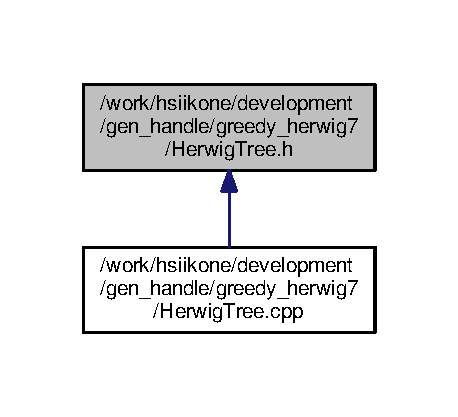
\includegraphics[width=220pt]{_herwig_tree_8h__dep__incl}
\end{center}
\end{figure}
\subsection*{Classes}
\begin{DoxyCompactItemize}
\item 
struct \hyperlink{struct_herwig_1_1_t_t_bar}{Herwig\+::\+T\+T\+Bar}
\begin{DoxyCompactList}\small\item\em A custom selector to be used with Herwig7. Not used, here for future reference. \end{DoxyCompactList}\item 
class \hyperlink{class_herwig_1_1_herwig_tree}{Herwig\+::\+Herwig\+Tree}
\begin{DoxyCompactList}\small\item\em The main class handle for the Herwig7 analysis. \end{DoxyCompactList}\end{DoxyCompactItemize}
\subsection*{Namespaces}
\begin{DoxyCompactItemize}
\item 
 \hyperlink{namespacesettings}{settings}
\begin{DoxyCompactList}\small\item\em A python-\/based script for generating a Herwig7 settings file. \end{DoxyCompactList}\item 
 \hyperlink{namespace_the_p_e_g}{The\+P\+EG}
\begin{DoxyCompactList}\small\item\em \hyperlink{namespace_the_p_e_g}{The\+P\+EG} is the basic infrastructure, on which Herwig7 is built. \end{DoxyCompactList}\item 
 \hyperlink{namespace_herwig}{Herwig}
\begin{DoxyCompactList}\small\item\em The standard Herwig7 namespace. \end{DoxyCompactList}\end{DoxyCompactItemize}
\subsection*{Functions}
\begin{DoxyCompactItemize}
\item 
bool \hyperlink{namespace_herwig_a894b97666725581816a4523a5cc1684d}{Herwig\+::\+Is\+Last\+In\+Shower} (const Particle \&p)
\end{DoxyCompactItemize}


\subsection{Detailed Description}
\begin{DoxyAuthor}{Author}
Hannu Siikonen (errai-\/ @Git\+Hub, hsiikone @Git\+Lab) 
\end{DoxyAuthor}
\begin{DoxyDate}{Date}
1.\+11.\+2017 (Last modification; fun times) 

1.\+11.\+2017 (Finishing touches for the greedy \hyperlink{namespace_herwig}{Herwig} 7 code) 

17.\+7.\+2018 (Fixed particle adding -\/\+Toni Mäkelä, tmakela @Git\+Lab) 
\end{DoxyDate}

\hypertarget{settings_8py}{}\section{/work/hsiikone/development/gen\+\_\+handle/greedy\+\_\+herwig7/settings.py File Reference}
\label{settings_8py}\index{/work/hsiikone/development/gen\+\_\+handle/greedy\+\_\+herwig7/settings.\+py@{/work/hsiikone/development/gen\+\_\+handle/greedy\+\_\+herwig7/settings.\+py}}
\subsection*{Namespaces}
\begin{DoxyCompactItemize}
\item 
 \hyperlink{namespacesettings}{settings}
\begin{DoxyCompactList}\small\item\em A python-\/based script for generating a Herwig7 settings file. \end{DoxyCompactList}\end{DoxyCompactItemize}
\subsection*{Variables}
\begin{DoxyCompactItemize}
\item 
list \hyperlink{namespacesettings_a8b4db2e0ad1b494a7e46577356f7a1b2}{settings.\+seeds}
\item 
int \hyperlink{namespacesettings_a3a71b954dc507b7c139f5a59def558ac}{settings.\+tune} = 0
\item 
float \hyperlink{namespacesettings_a041ea5ae27a35144e20d819d903e242f}{settings.\+min\+KT} = 20.\+0
\item 
float \hyperlink{namespacesettings_a9c21d19d19519afd9c32d6c6c8cd7be5}{settings.\+m\+Top} = 175.\+0
\item 
int \hyperlink{namespacesettings_acf9ea9fa8fde8d823a80f50e2059d636}{settings.\+pdf} = 3
\item 
int \hyperlink{namespacesettings_ae5853b0ece109429ba3e5fdbbaea4cb3}{settings.\+e\+Scale} = 2
\item 
bool \hyperlink{namespacesettings_a594c41de23324522b6d9c80046032a95}{settings.\+hepmc} = False
\item 
bool \hyperlink{namespacesettings_a35611de950cb2fb15983284123fa724c}{settings.\+I\+SR} = True
\item 
bool \hyperlink{namespacesettings_ac98d9a0de50c24fd4cc8ca6329a3e0c6}{settings.\+F\+SR} = True
\item 
bool \hyperlink{namespacesettings_aa5b9f7d5c3011f7d0e4390a0955190e2}{settings.\+M\+PI} = True
\item 
bool \hyperlink{namespacesettings_a73303983a691070f10b880f7a5960a39}{settings.\+Weighting} = True
\item 
\hyperlink{namespacesettings_a05f6f4b8d16087cff8c66baecd6b9526}{settings.\+tot\+\_\+evts} = int(sys.\+argv\mbox{[}1\mbox{]})
\item 
\hyperlink{namespacesettings_a51b31b0cdbe61e6cd2f758e8560898e9}{settings.\+mode} = int(sys.\+argv\mbox{[}2\mbox{]})
\item 
\hyperlink{namespacesettings_ae0c0aa2289384505ec166c1b20c0f98c}{settings.\+procs} = int(sys.\+argv\mbox{[}3\mbox{]})
\item 
\hyperlink{namespacesettings_a3f99a62963c1c5a80e211f1507f4c8b0}{settings.\+proc\+\_\+id} = int(sys.\+argv\mbox{[}4\mbox{]})
\item 
string \hyperlink{namespacesettings_a503a5b5d5affd77fa0d769a08bc95a13}{settings.\+name} = \char`\"{}\char`\"{}
\item 
\hyperlink{namespacesettings_a7f8f246eb917372c33fb5f296093ff70}{settings.\+f} = open(name,\textquotesingle{}w\textquotesingle{})
\end{DoxyCompactItemize}

\input{greedy__settings_8h}
%--- End generated contents ---

% Index
\backmatter
\newpage
\phantomsection
\clearemptydoublepage
\addcontentsline{toc}{chapter}{Index}
\printindex

\end{document}
